\section{Training Dynamics}

In this section, we study the trajectories $\bm \theta(t)$ that are solutions of the gradient flow~\eqref{eq:gradient_flow}. As noted in~\cite{NTKJacot}, given a trajectory $\bm \theta(t)$, we can decribe the corresponding path in functional space $f_{\bm \theta(t)}$ using the \emph{tangent kernel} (at least when $\bm \theta$ is in the interior of some activation region $R(\bm \tau,\bm \epsilon)$). In our setting, we consider the map $\Psi: \bm \theta \mapsto {\bm {\hat y}} = (f_{\bm \theta}(x_1),\ldots,f_{\bm \theta}(x_s))$, and have that
\begin{equation}\label{eq:tangent_kernel}
\begin{aligned}
    {\bm {\hat y}}'(t) &= J \Psi(\bm \theta(t)) \cdot J \Psi(\bm \theta(t))^T \cdot \bm r(t)\\
    &= [J_{\bm c} \Psi(\bm \theta(t)) \cdot J_{\bm c} \Psi(\bm \theta(t))^T + J_{\bm a} \Psi(\bm \theta(t)) \cdot J_{\bm a} \Psi(\bm \theta(t))^T + J_{\bm b} \Psi(\bm \theta(t)) \cdot J_{\bm b} \Psi(\bm \theta(t))^T] \cdot \bm r(t)\\
    &= (\bm M_{\bm a\bm b} \bm M_{\bm a\bm b}^T + \bm N^{(1)}_{\bm \tau \bm c} {\bm N_{\bm \tau \bm c}^{(1)T}} + \bm N^{(2)}_{\bm \tau \bm c} {\bm N_{\bm \tau \bm c}^{(2)T}}) \cdot \bm r(t)\\
    & = (\bm K^{\bm c} + \bm K^{\bm a\bm b}) \cdot \bm r(t),
\end{aligned}
\end{equation}
where $\bm r(t) = \bm{\hat y}(t) - \bm y(t)$ is the vector of residuals, and
\begin{equation}
    \bm K^{\bm c}= \bm M_{\bm a\bm b} \bm M_{\bm a\bm b}^T, \qquad
    \bm K^{\bm a \bm b} = \bm N^{(1)}_{\bm \tau \bm c} {\bm N_{\bm \tau \bm c}^{(1)T}} + \bm N^{(2)}_{\bm \tau \bm c} {\bm N_{\bm \tau \bm c}^{(2)T}},
\end{equation}
\begin{equation}
    \bm M_{\bm a\bm b} = [\tau_{ij}(a_j x_i + b_j)]_{ij} \in \RR^{s \times m}, \quad \bm N_{\bm \tau \bm c}^{(1)}= [c_j \tau_{ij} x_i]_{ij} \in \RR^{s \times m},
    \quad \bm N_{\bm \tau \bm c}^{(2)} = [c_j \tau_{ij}]_{ij} \in \RR^{s \times m}.
\end{equation}
The symmetric matrices (kernels) $\bm K^{(c)}$ and $\bm K^{(a,b)}$ in~\eqref{eq:tangent_kernel} describe the trajectory of the predictor $\bm {\hat y}$, but are not constant throughout time. As we argue below, $\bm K^{(c)}$ and $\bm K^{(a,b)}$ affect the trajectory in very different ways: if $\bm K^{(c)}$ ``dominates'' in ~\eqref{eq:tangent_kernel}, we are in the regime of \emph{kernel learning}, for which the bottom layer parameters ($\bm a, \bm b$) are roughly fixed; when instead $\bm K^{(a, b)}$ dominates, then the top layer parameter $\bm c$ is roughly fixed, and we are in a regime that we refer to as \emph{purely adaptive learning}.
In the next subsection, we explain how both extreme regimes can occur at any point in function/predictor space, depending on the initialization of the parameters.
\note{We don't really use this, but maybe it's good to make a clear connection with NTK/lazy learning. Maybe we can shorten it though}

\subsection{Dynamics in reduced parameters}

The matrices $\bm K^{\bm c}$ and $\bm K^{\bm ab}$ depend on the value of the parameters $\bm \theta = (\bm a, \bm b, \bm c)$, and it is in fact easy to realize that they are not constant in a \emph{fiber} of the map $\bm \theta \rightarrow f_{\bm \theta}$, \ie, among the set of parameters representing the same function. This means that even if $\bm \theta_0, \bm \theta_0'$ are such that $f_{\bm \theta_0} = f_{\bm \theta_0'}$, the gradient flow~\eqref{eq:gradient_flow} for $\bm \theta(0) = \bm \theta_0$ or $\bm \theta(0) = \bm \theta_0'$ can converge to very different functions (see Figure~\ref{fig:different_funcs_same_init}). Thus we cannot use the initial state directly to categorize the types of trajectories in the fiber. Instead, the following conserved quantity (which depends only on $\bm \theta_0$) categorizes the trajectory of $\bm \theta(t)$:

\begin{lemma} \label{le:fixed_delta}
If $\bm \theta(t) = (\bm a(t), \bm b(t), \bm c(t))$ is a solution of the integral flow \eqref{eq:gradient_flow}, then the quantities
\begin{equation}\label{eq:invariants}
\delta_i = c_i(t)^2 - a_i(t)^2 - b_i(t)^2, \quad i = 1, \ldots, m,
\end{equation}
remain constant for all $t$. In particular, given a reduced representation of a neuron $(u_i,v_i) = (|c_i|a_i,|c_i|b_i)$, we can recover the original neuron $(a_i,b_i,c_i)$ up to the sign of $c_i$, since
\begin{equation}\label{eq:c_uv}
    c_i^2 = \frac{\delta_i + \sqrt{\delta_i^2 + 4 (u_i^2 + v_i^2)}}{2}. 
\end{equation}
\end{lemma}

We next assume that $\bm \theta$ is a parameter in the interior of an activation region $R(\bm \tau, \bm \epsilon)$. We define the \emph{loss in reduced parameters} \note{Notation?}
\begin{equation}
    \tilde L(\bm \xi) = \sum_{i=1}^s |g_{\bm \epsilon, \bm \xi}(x_i) - y_i|^2, \qquad \bm \xi = (\bm u, \bm v) \in \RR^{2m},  
\end{equation}
\begin{equation}
    g_{\bm \epsilon,\bm \xi}(x) = \sum_{j=1}^m \epsilon_i [ u_i x + v_i]_+.
\end{equation}
Inside $R(\bm \tau,\bm \epsilon)$ (where the sign vector $\bm \epsilon$ is fixed) the gradient of the loss in reduced parameters $\nabla \tilde L(\bm \xi)$ is very simple: indeed, the association $\bm \xi \rightarrow (g_{\bm \xi}(x_1),\ldots,g_{\bm \xi}(x_s))$ is \emph{linear}, since $g_{\bm \xi}(x_i) = \sum_{i=1}^m \tau_{ij} \epsilon_j (u_j x_i + v_j)$, so the field $\nabla \tilde L(\bm \xi)$ points in a unique direction (see Figure~\ref{fig:reduced_grad})

\begin{theorem}\label{thm:reduced_parameter_grad}
Let $\bm \theta(t)$ be an integral curve for the gradient flow \eqref{eq:gradient_flow} of $L(\bm \theta)$, and let $\bm \delta = (\delta_i) \in \RR^m$ be the vector of invariants~\eqref{eq:invariants}, which depend only on the initialization $\bm \theta(0)$. If $\bm \xi(t) = (\bm u(t), \bm v(t))$ is curve of reduced parameters corresponding to $\bm \theta(t)$, then we have that
\begin{equation}
\begin{bmatrix}
\dot u_i(t)\\
\dot v_i(t)
\end{bmatrix} =
\bm P_{\delta_i}(u_i,v_i)
\begin{bmatrix}
\nabla_{u_i} \tilde L (\bm \xi)\\
\nabla_{v_i} \tilde L (\bm \xi)\\
\end{bmatrix},
\quad i=1,\ldots,m,
\end{equation}
where
\begin{equation}\label{eq:neuron_kernel}
\bm P_\delta(u_i,v_i) = \begin{bmatrix}
    a_i^2 + c_i^2  & 
    a_i b_i        \\
    a_i b_i               & 
    b_i^2 + c_i^2\\
\end{bmatrix} = 
\begin{bmatrix}
\frac{u_i^2}{c(u_i, v_i)^2} + c(u_i, v_i)^2 & \frac{u_i v_i}{c(u_i, v_i)^2}\\
\frac{u_i v_i}{c(u_i, v_i)^2} &  \frac{v_i^2}{c(u_i, v_i)^2} + c(u_i, v_i)^2\\
\end{bmatrix},
\end{equation}

and $c(u_i, v_i)^2 = \frac{\delta_i + \sqrt{\delta_i^2 + 4 (u_i^2 + v_i^2)}}{2}$
\end{theorem}




% We also explore the special case of \emph{lazy training} (\cite{NTKJacot}, \cite{chizat2018note}) where the parameters of the first layer ($a$ and $b$) are fixed and the parameters of the outer layer ($c$) are allowed to move. We show that in the lazy regime, the solution to gradient descent is a natural cubic spline.


This Theorem shows how the dynamics of a (reduced) neuron are related to the simpler (locally linear) dynamics of the reduced loss. It is easy to verify that the eigenvalue-eigenvector pairs of $\bm P_{\delta_i}(u_i,v_i)$ are
\begin{align}
    (\lambda_1, \bm w_1) &= (a_i^2+ b_i^2 + c_i^2, (u_i,v_i))
    % = \left(\frac{1}{c^2}(\beta(a^2 + b^2) + \alpha), \left(\frac{u}{|c|}, \frac{v}{|c|}\right)\right)
    \label{eq:radial_eigenval}\\
    (\lambda_2, \bm w_2) &= (c_i^2, (-v_i,u_i)) 
    % = \left(\alpha c^2, \left(-\frac{v}{|c|}, \frac{v}{|c|}\right)\right)
    \label{eq:tangential_eigenval}
\end{align}
The eigenvectors of $\bm P_{\delta_i}(u_i,v_i)$ define two extreme trajectories, and we can understand the dynamics of a neuron as a continuum between these extrema. In fact, writing $\rho_i = u_i^2 + v_i^2$, it is straightforward to verify that:

\begin{itemize}
    \item If $\rho_i \ll |\delta_i|$ and $\delta < 0$, then $\xi'(t) \propto \xi$, and the neuron moves \emph{radially}.
    \item If $\rho_i \ll |\delta_i|$ and $\delta > 0$, then $(\dot u_i(t), \dot v_i(t)) \propto \nabla_{u_i} \tilde L(\bm \xi(t))$, so the reduced neuron moves parallel to the vector field $\nabla \tilde L(\bm \xi)$.
\end{itemize}
It is also interesting to note that the trajectories of neurons follow paths that are (up to rotations) solutions to one of two possible ODEs: indeed, we can always assume $\bm \delta_i = \pm 1$ given that
\begin{equation}
\bm P_{\delta_i}(u_i,v_i)\cdot v = \bm P_{\delta_i/|\delta_i|} \left(\frac{u_i}{|\delta_i|},\frac{v_i}{|\delta_i|}\right) \cdot |\delta_i|v.
\end{equation}
This means the trajectory of a neuron can be understood locally by considering the vector field $\bm P_{\pm 1}(u_i,v_i) \cdot \nabla \tilde{L}(\bm \xi)$ at a different (rescaled) point. \note{Show figure of the two vector fields}

\begin{figure}\label{fig:trajectories}
    \centering
    \minipage{0.33\textwidth}
    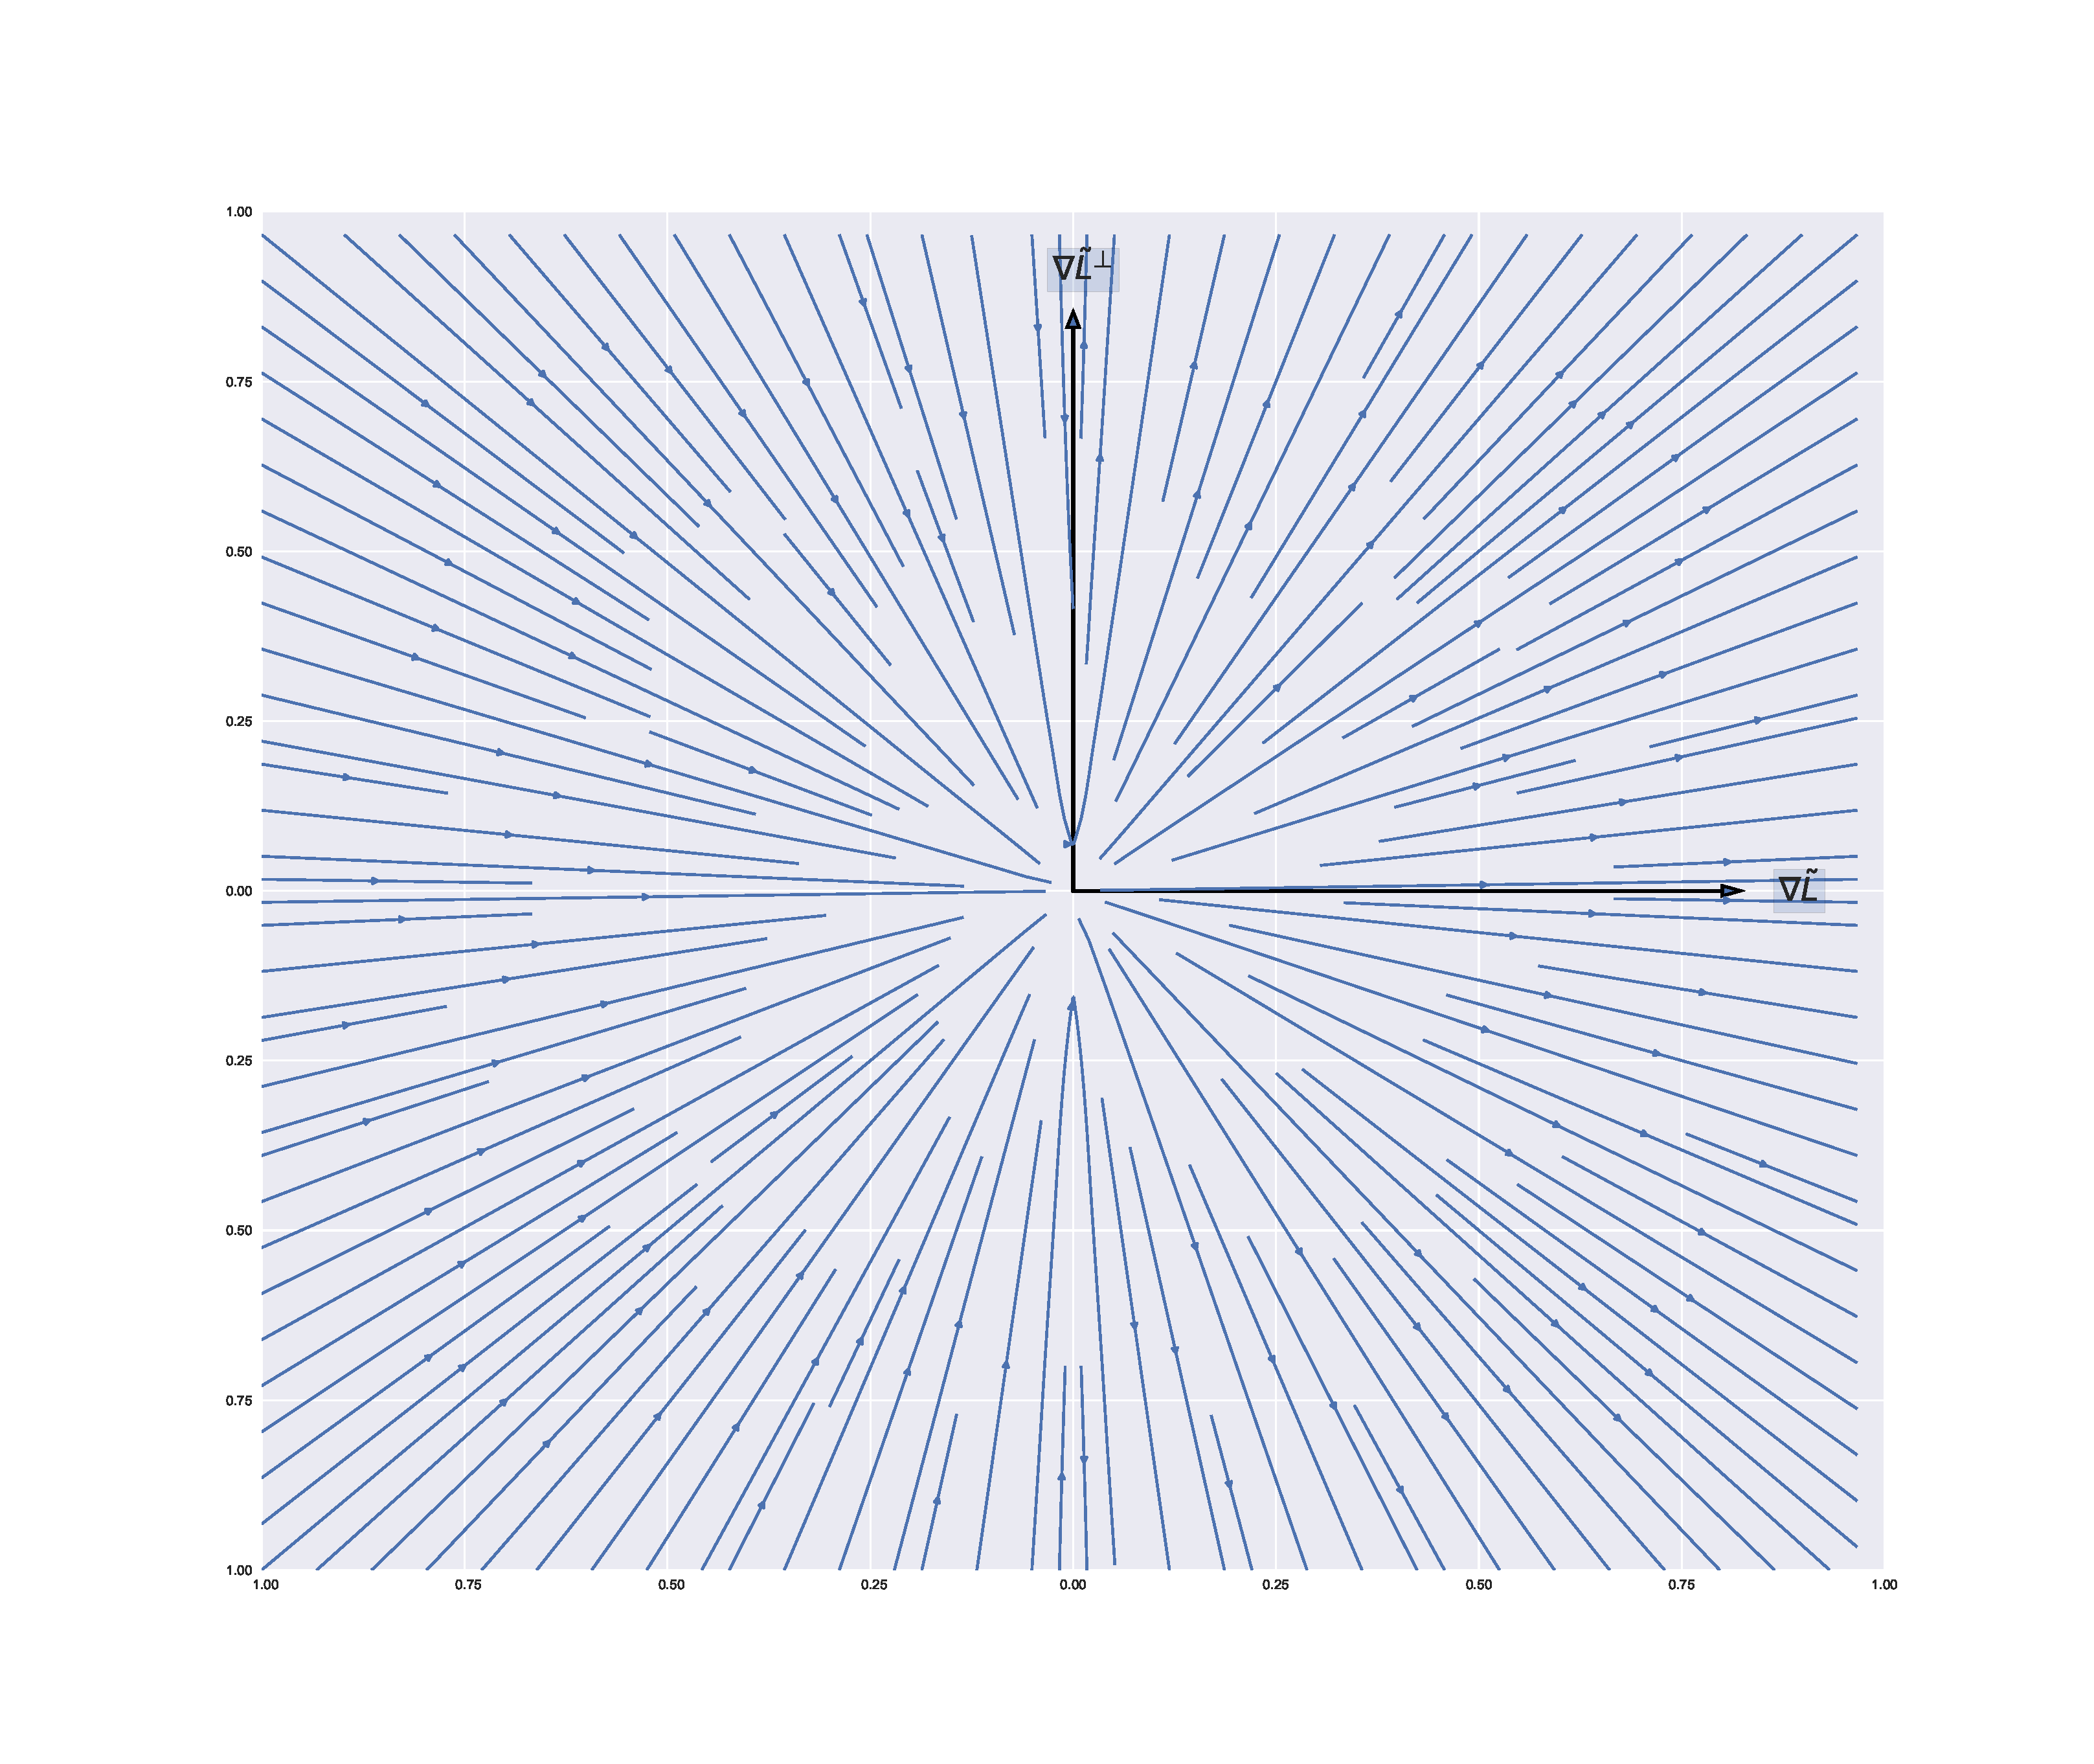
\includegraphics[width=\linewidth]{figures/dynamics_delta_-100.pdf}
    \endminipage\hfill
    % \minipage{0.2\textwidth}
    % 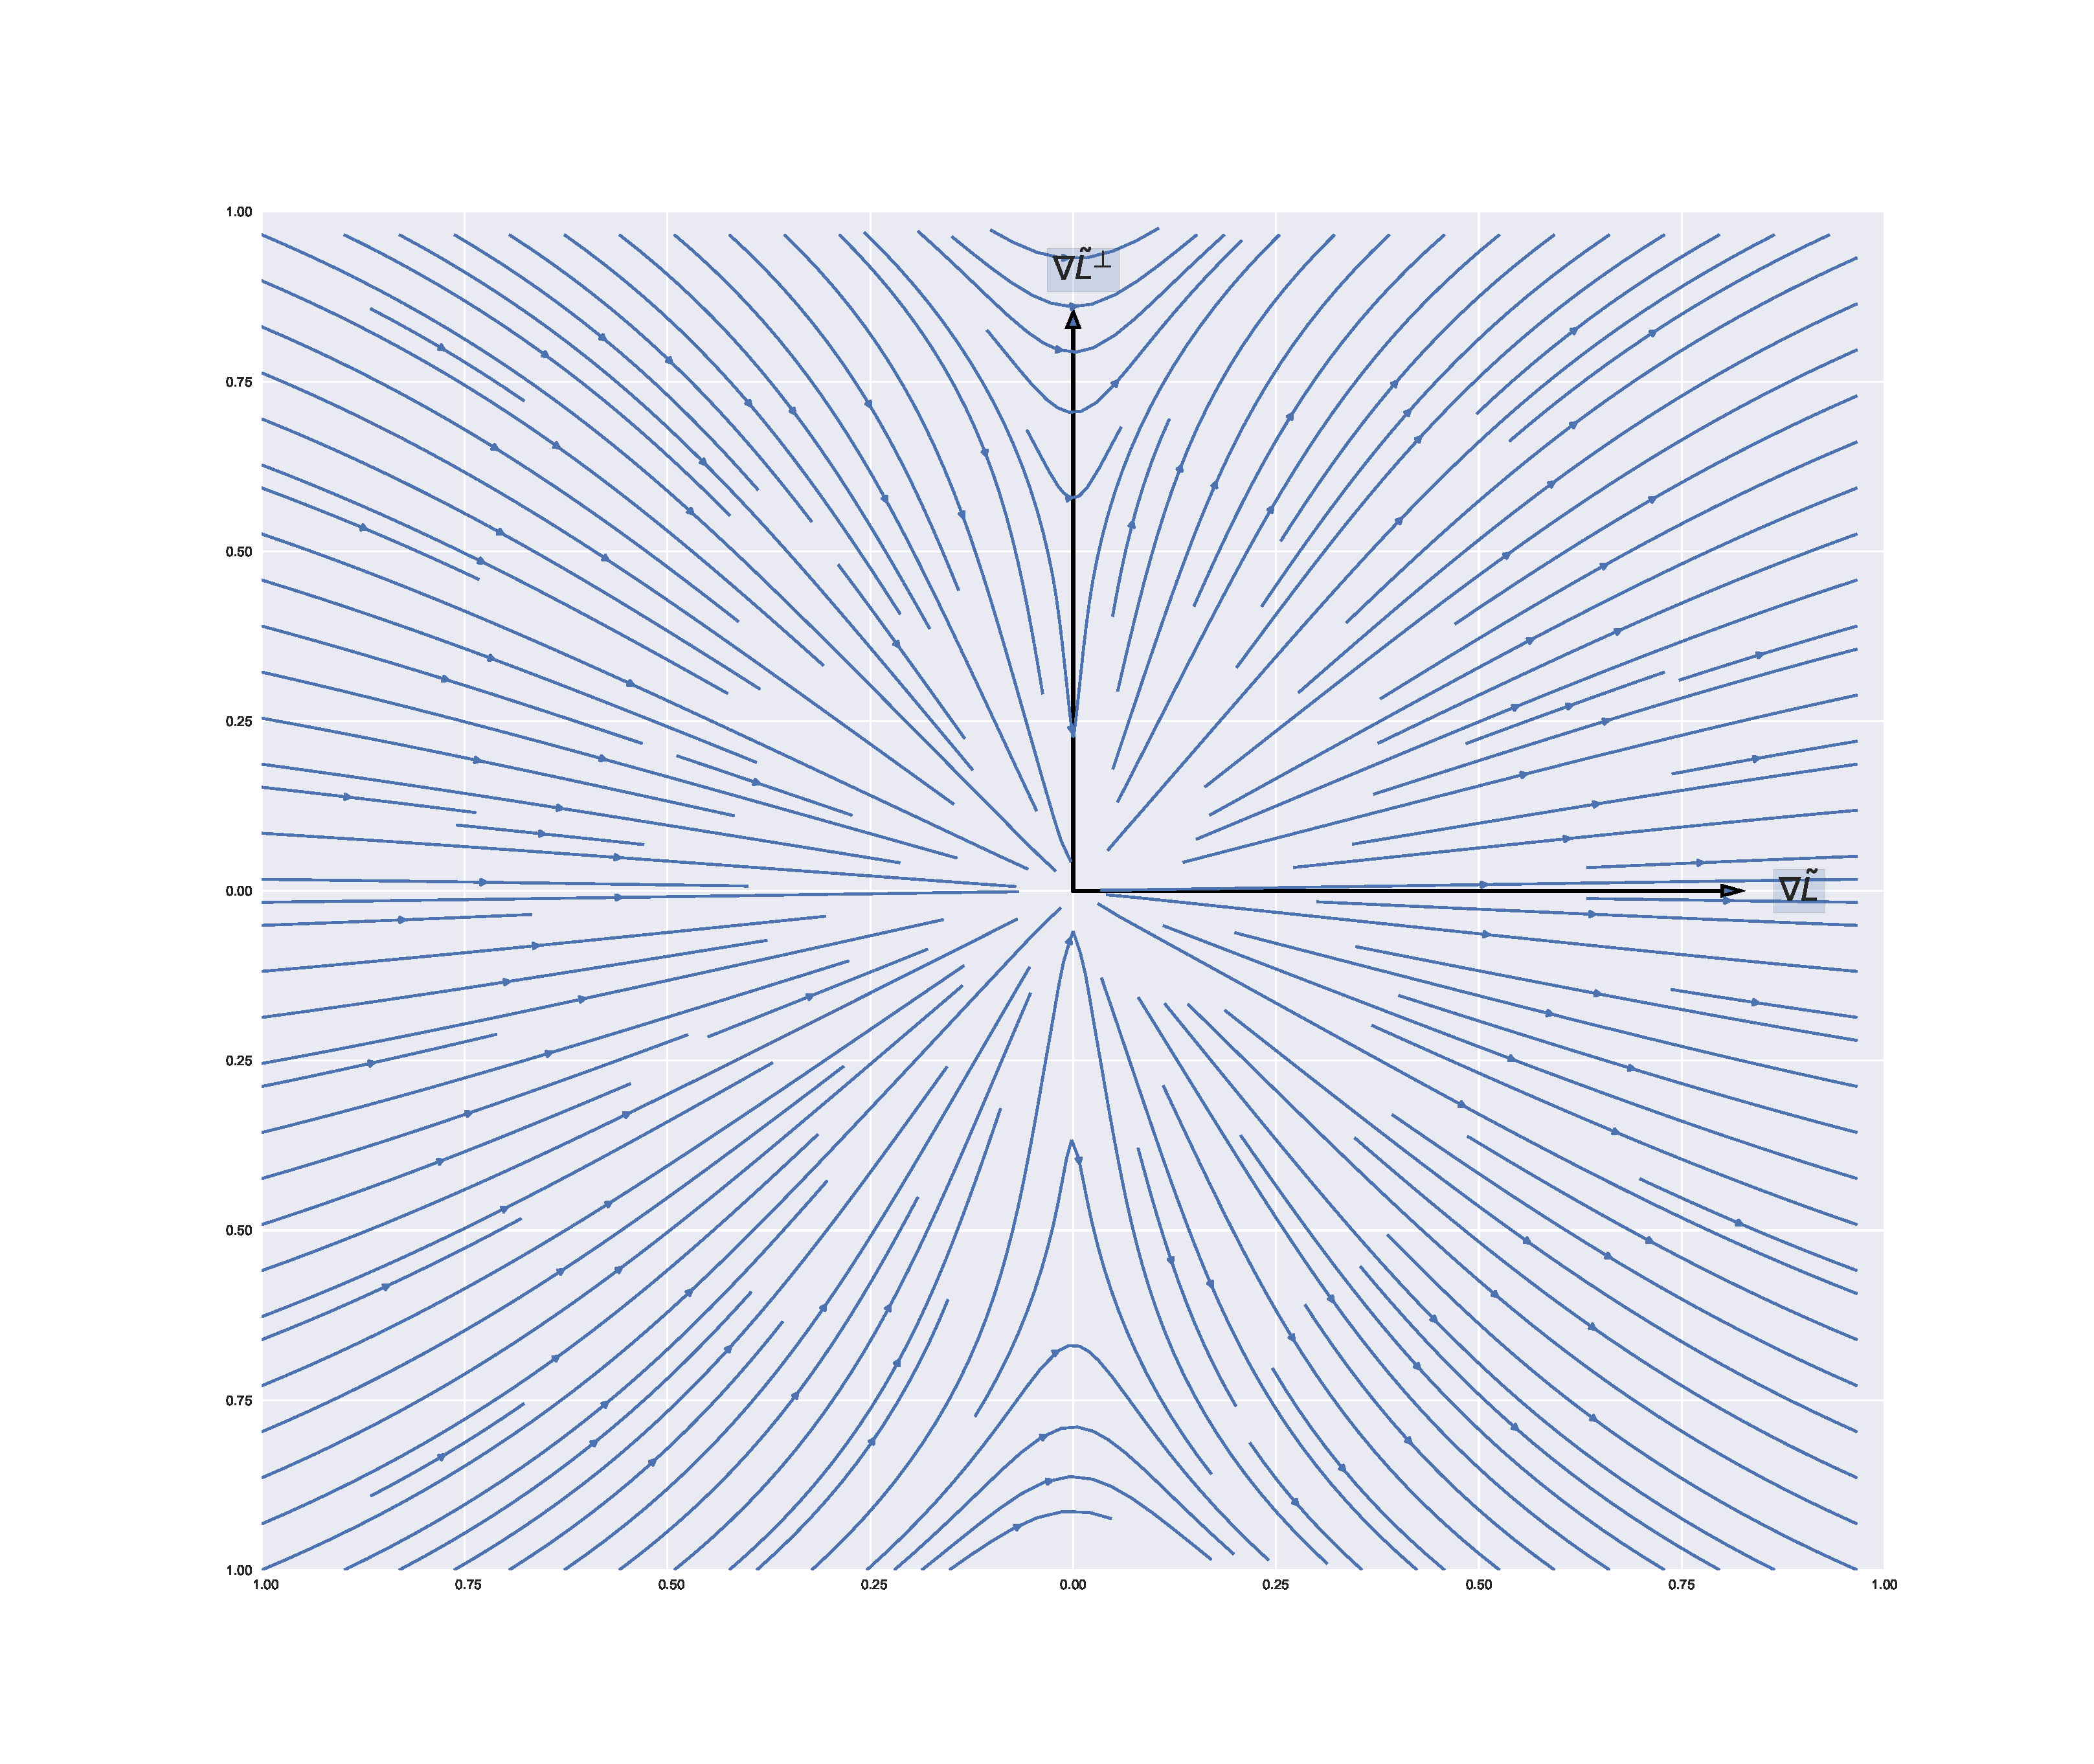
\includegraphics[width=\linewidth]{figures/dynamics_delta_-1.pdf}
    % \endminipage\hfill
    \minipage{0.33\textwidth}
    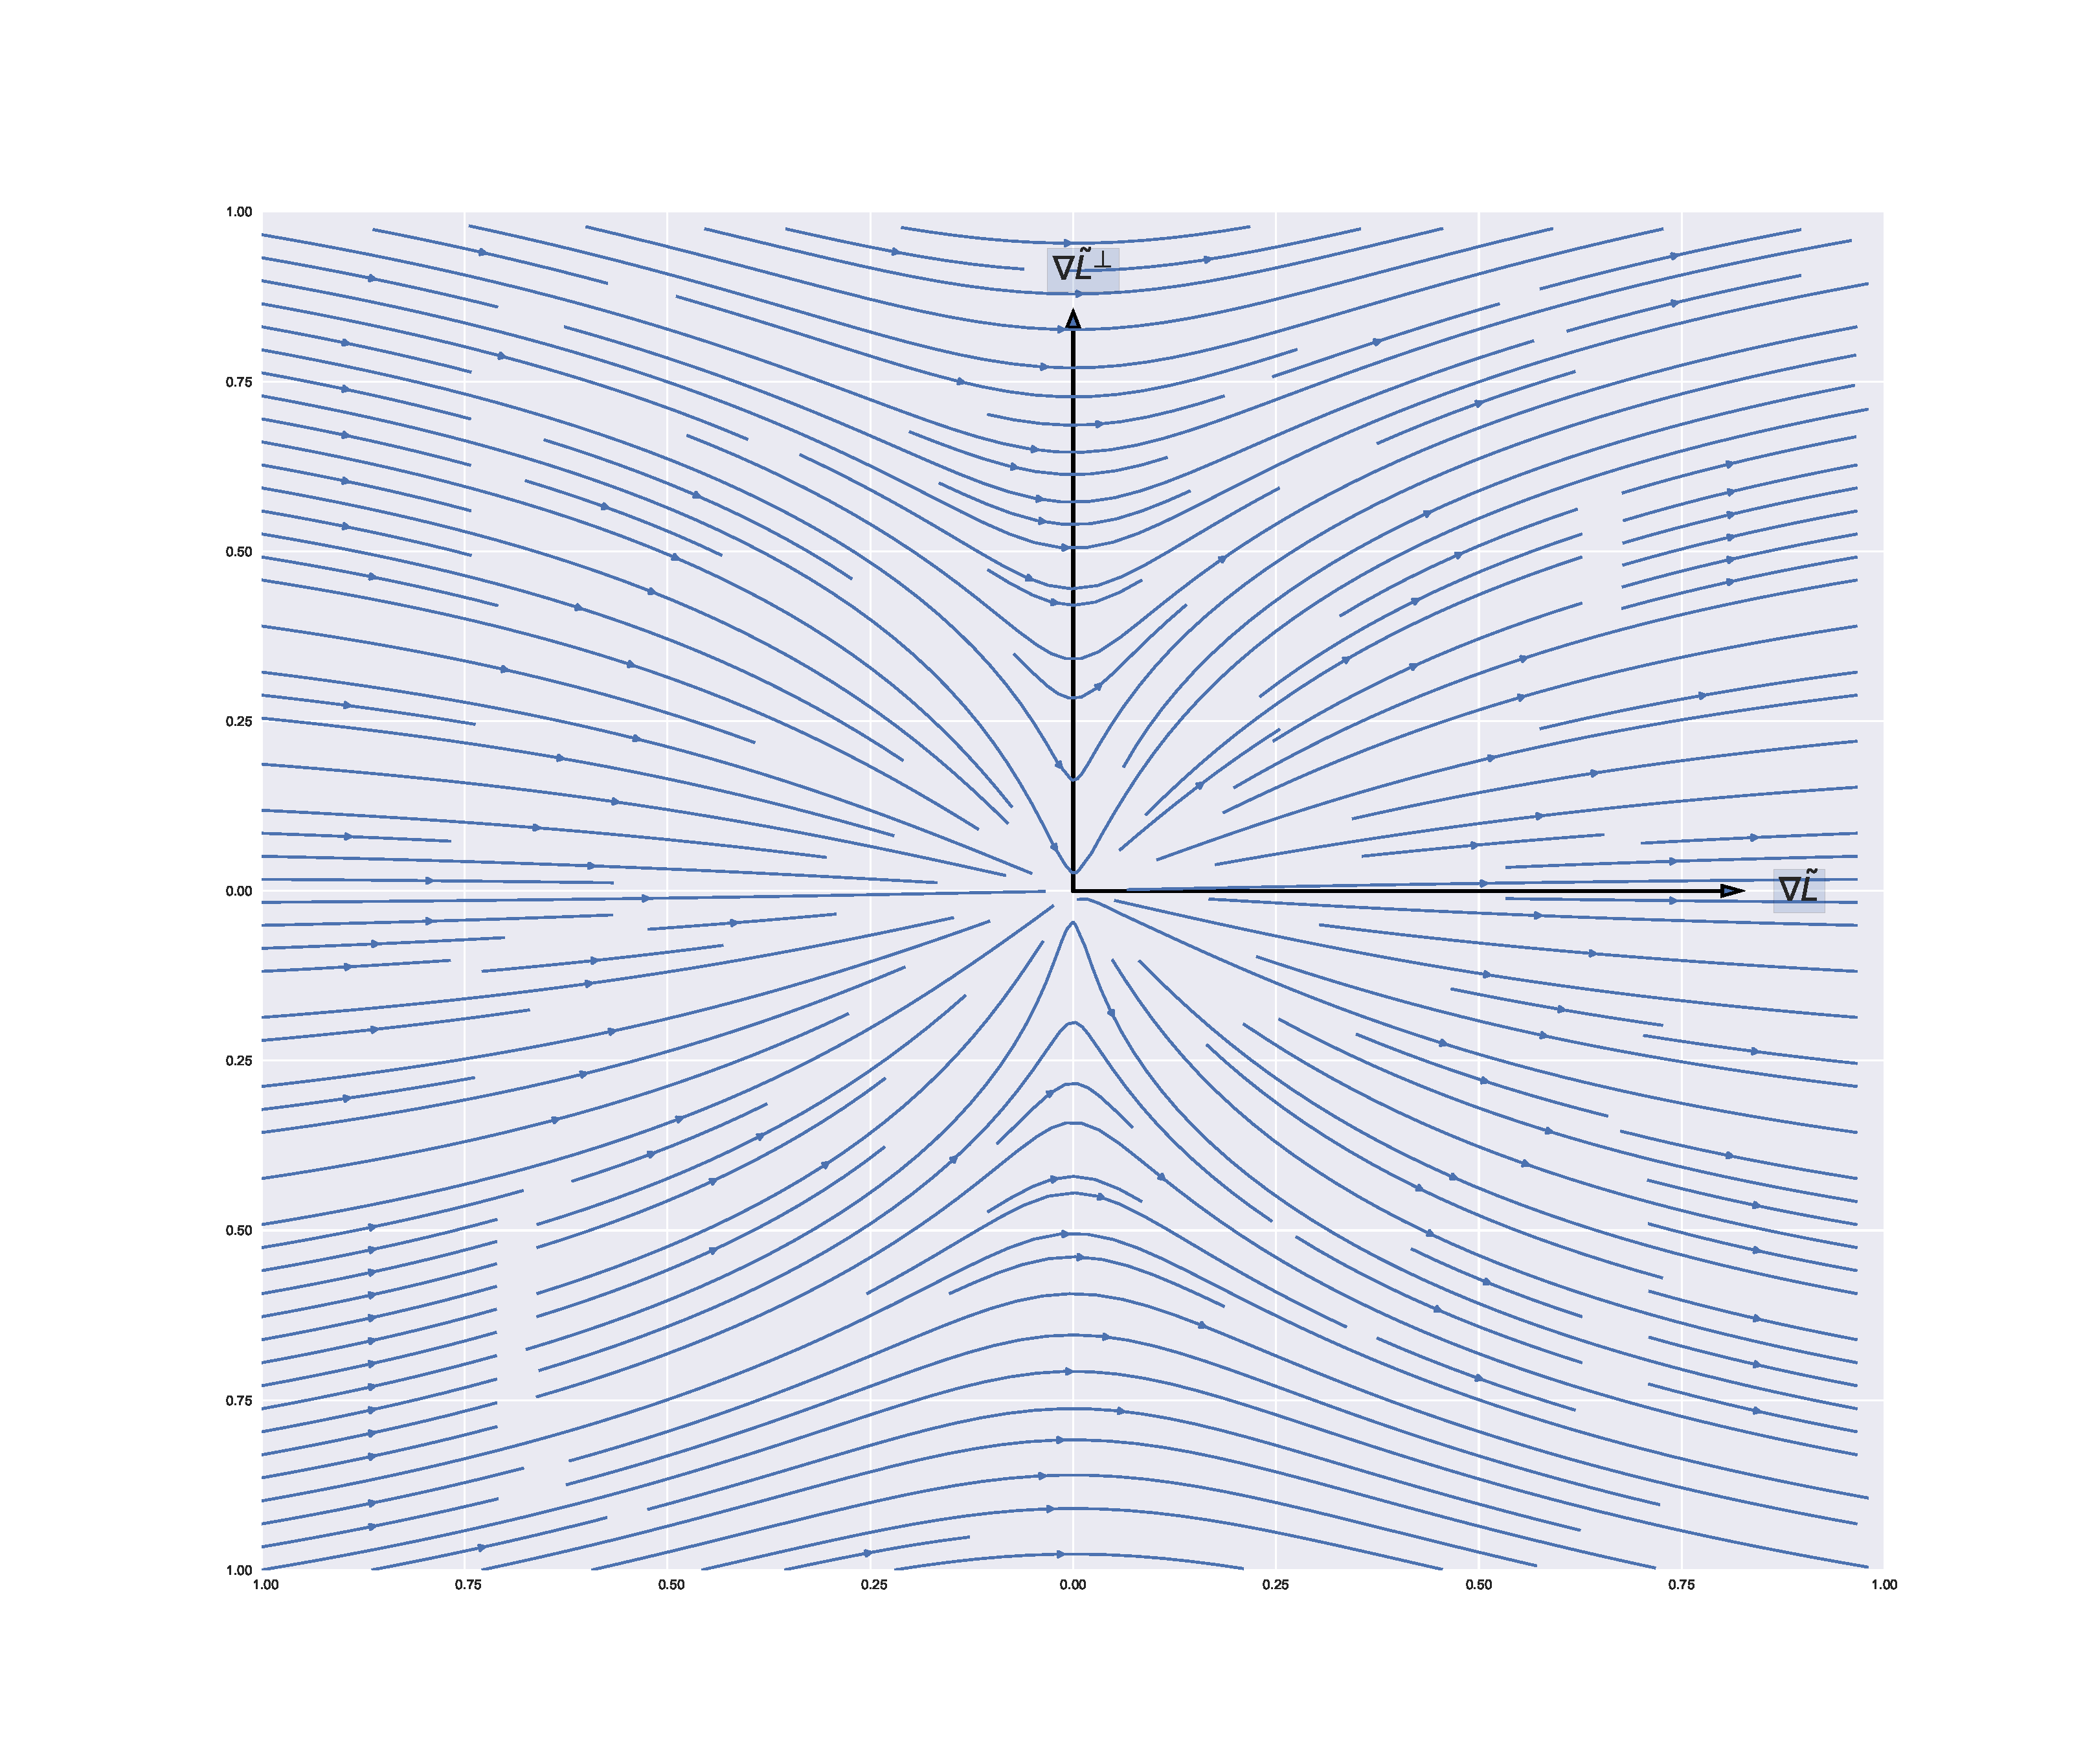
\includegraphics[width=\linewidth]{figures/dynamics_delta_0.pdf}
    \endminipage\hfill
    % \minipage{0.2\textwidth}
    % 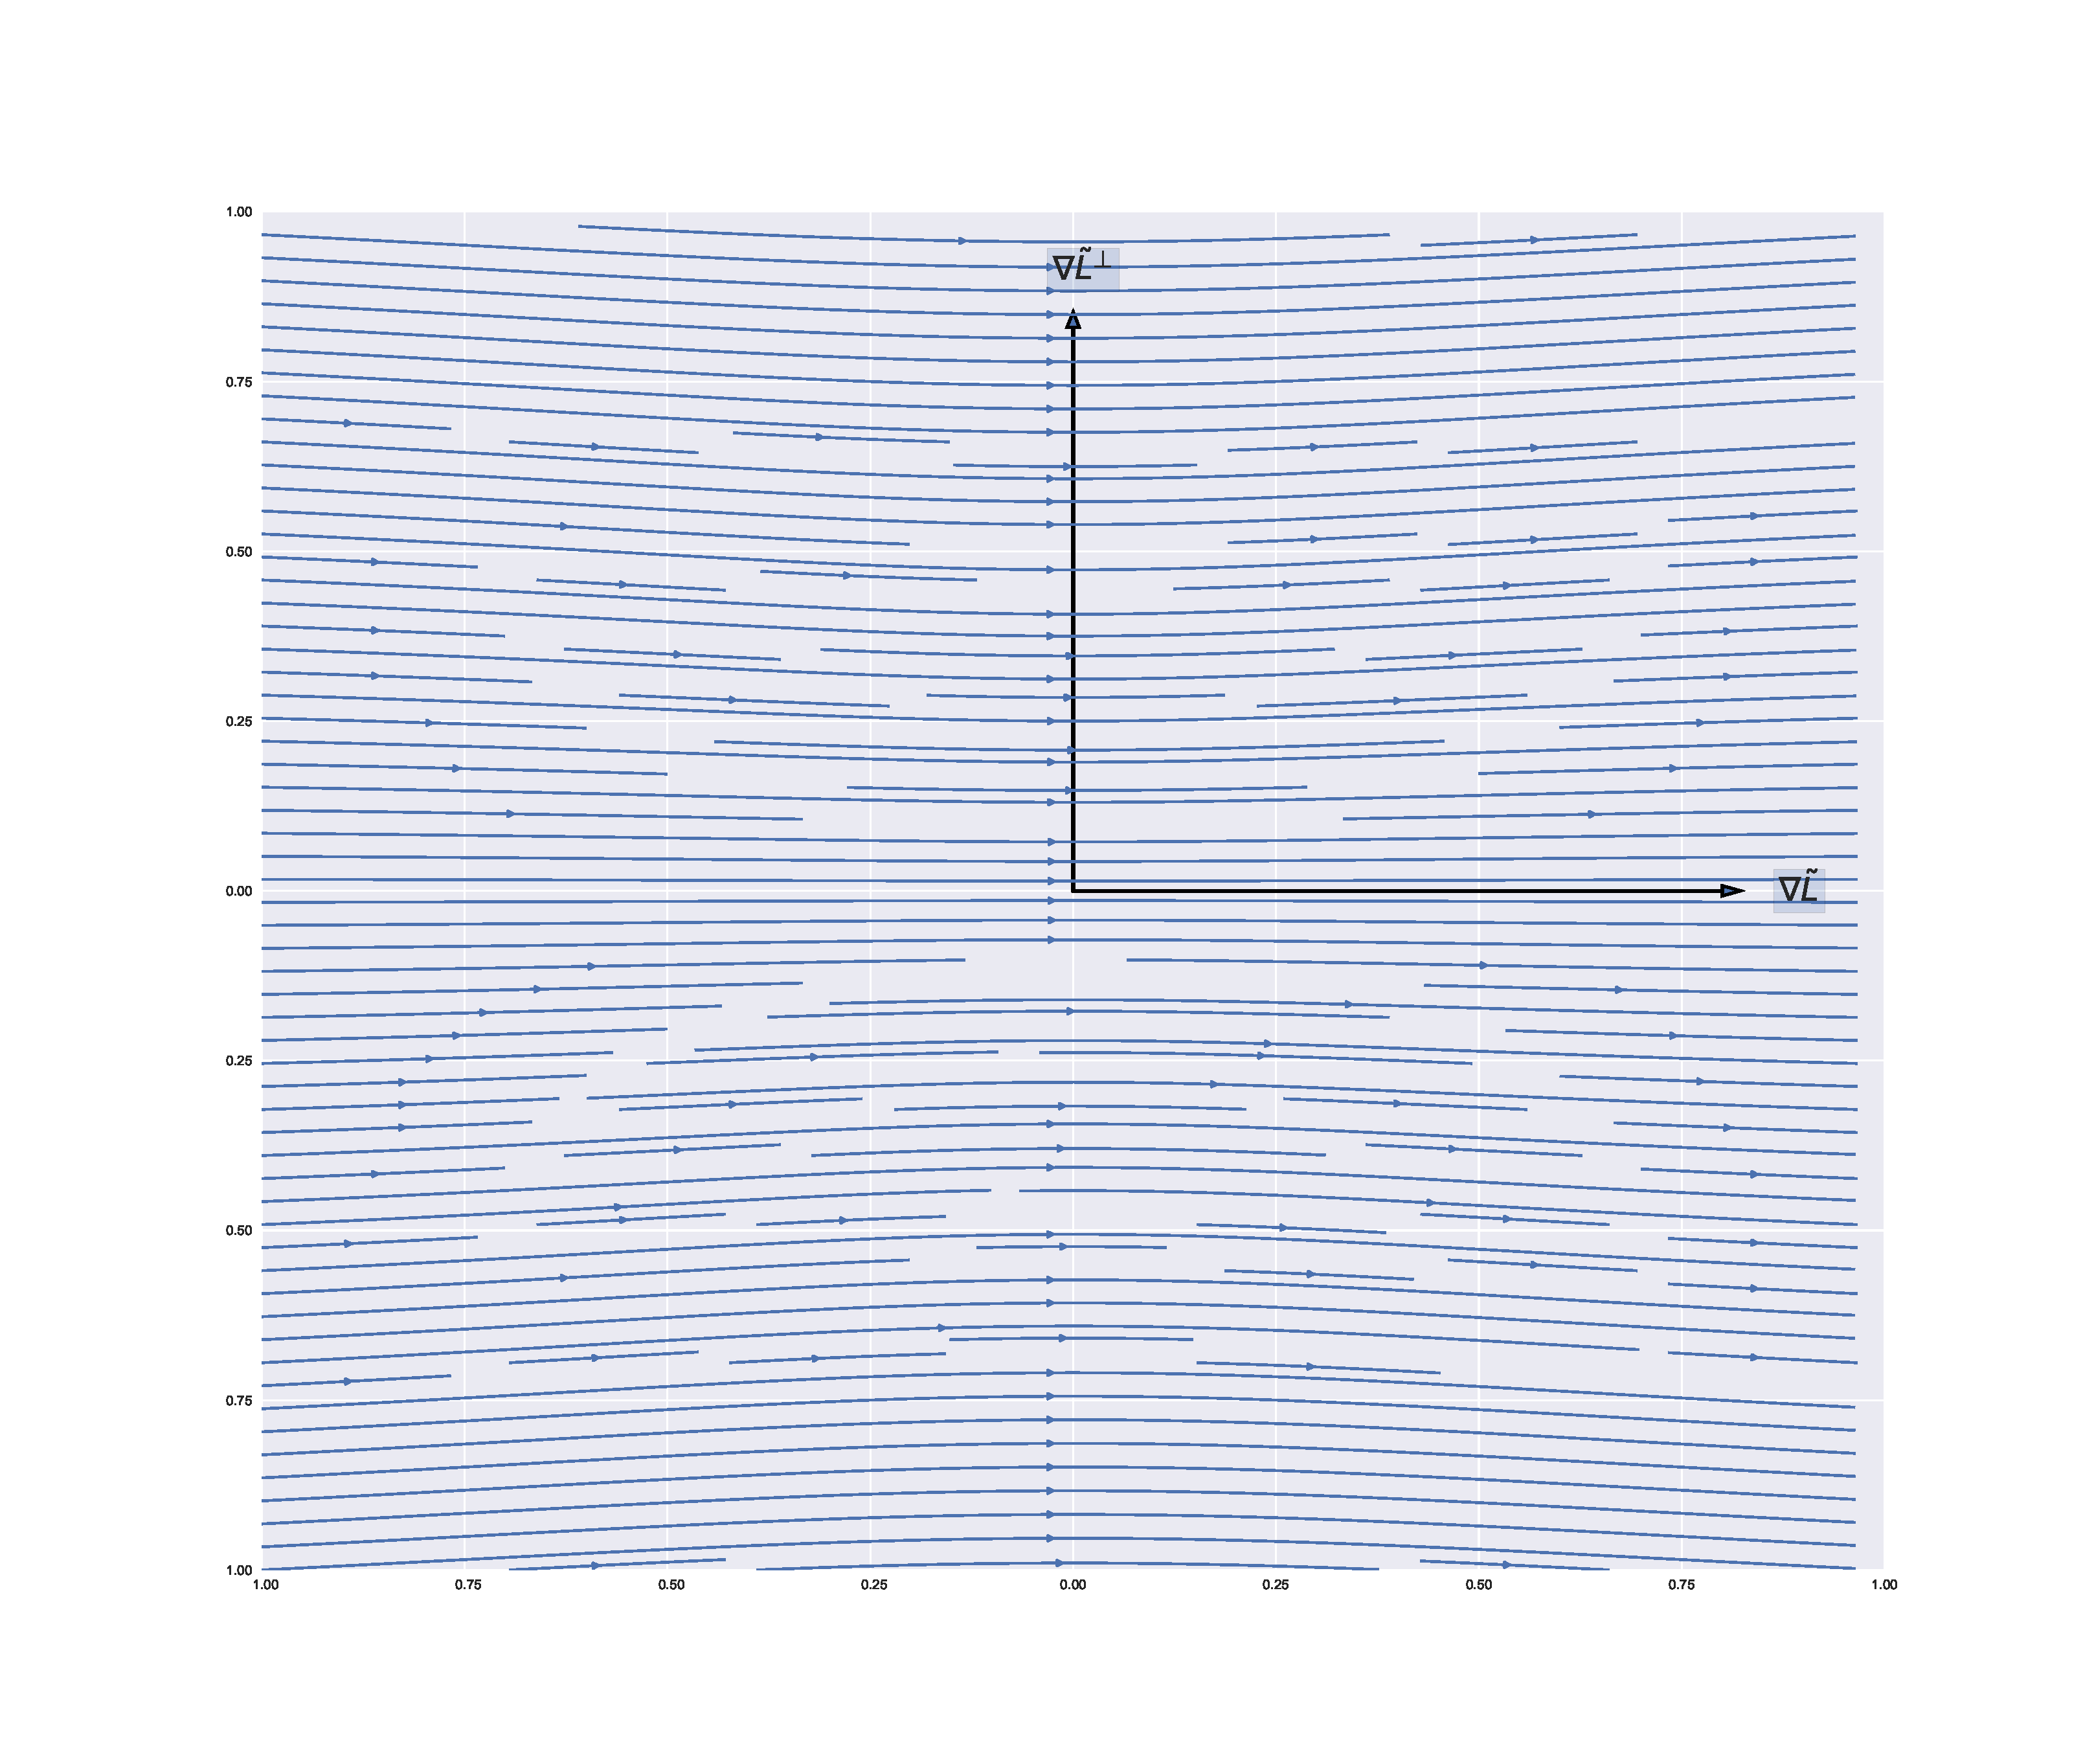
\includegraphics[width=\linewidth]{figures/dynamics_delta_1.pdf}
    % \endminipage\hfill
    \minipage{0.33\textwidth}
    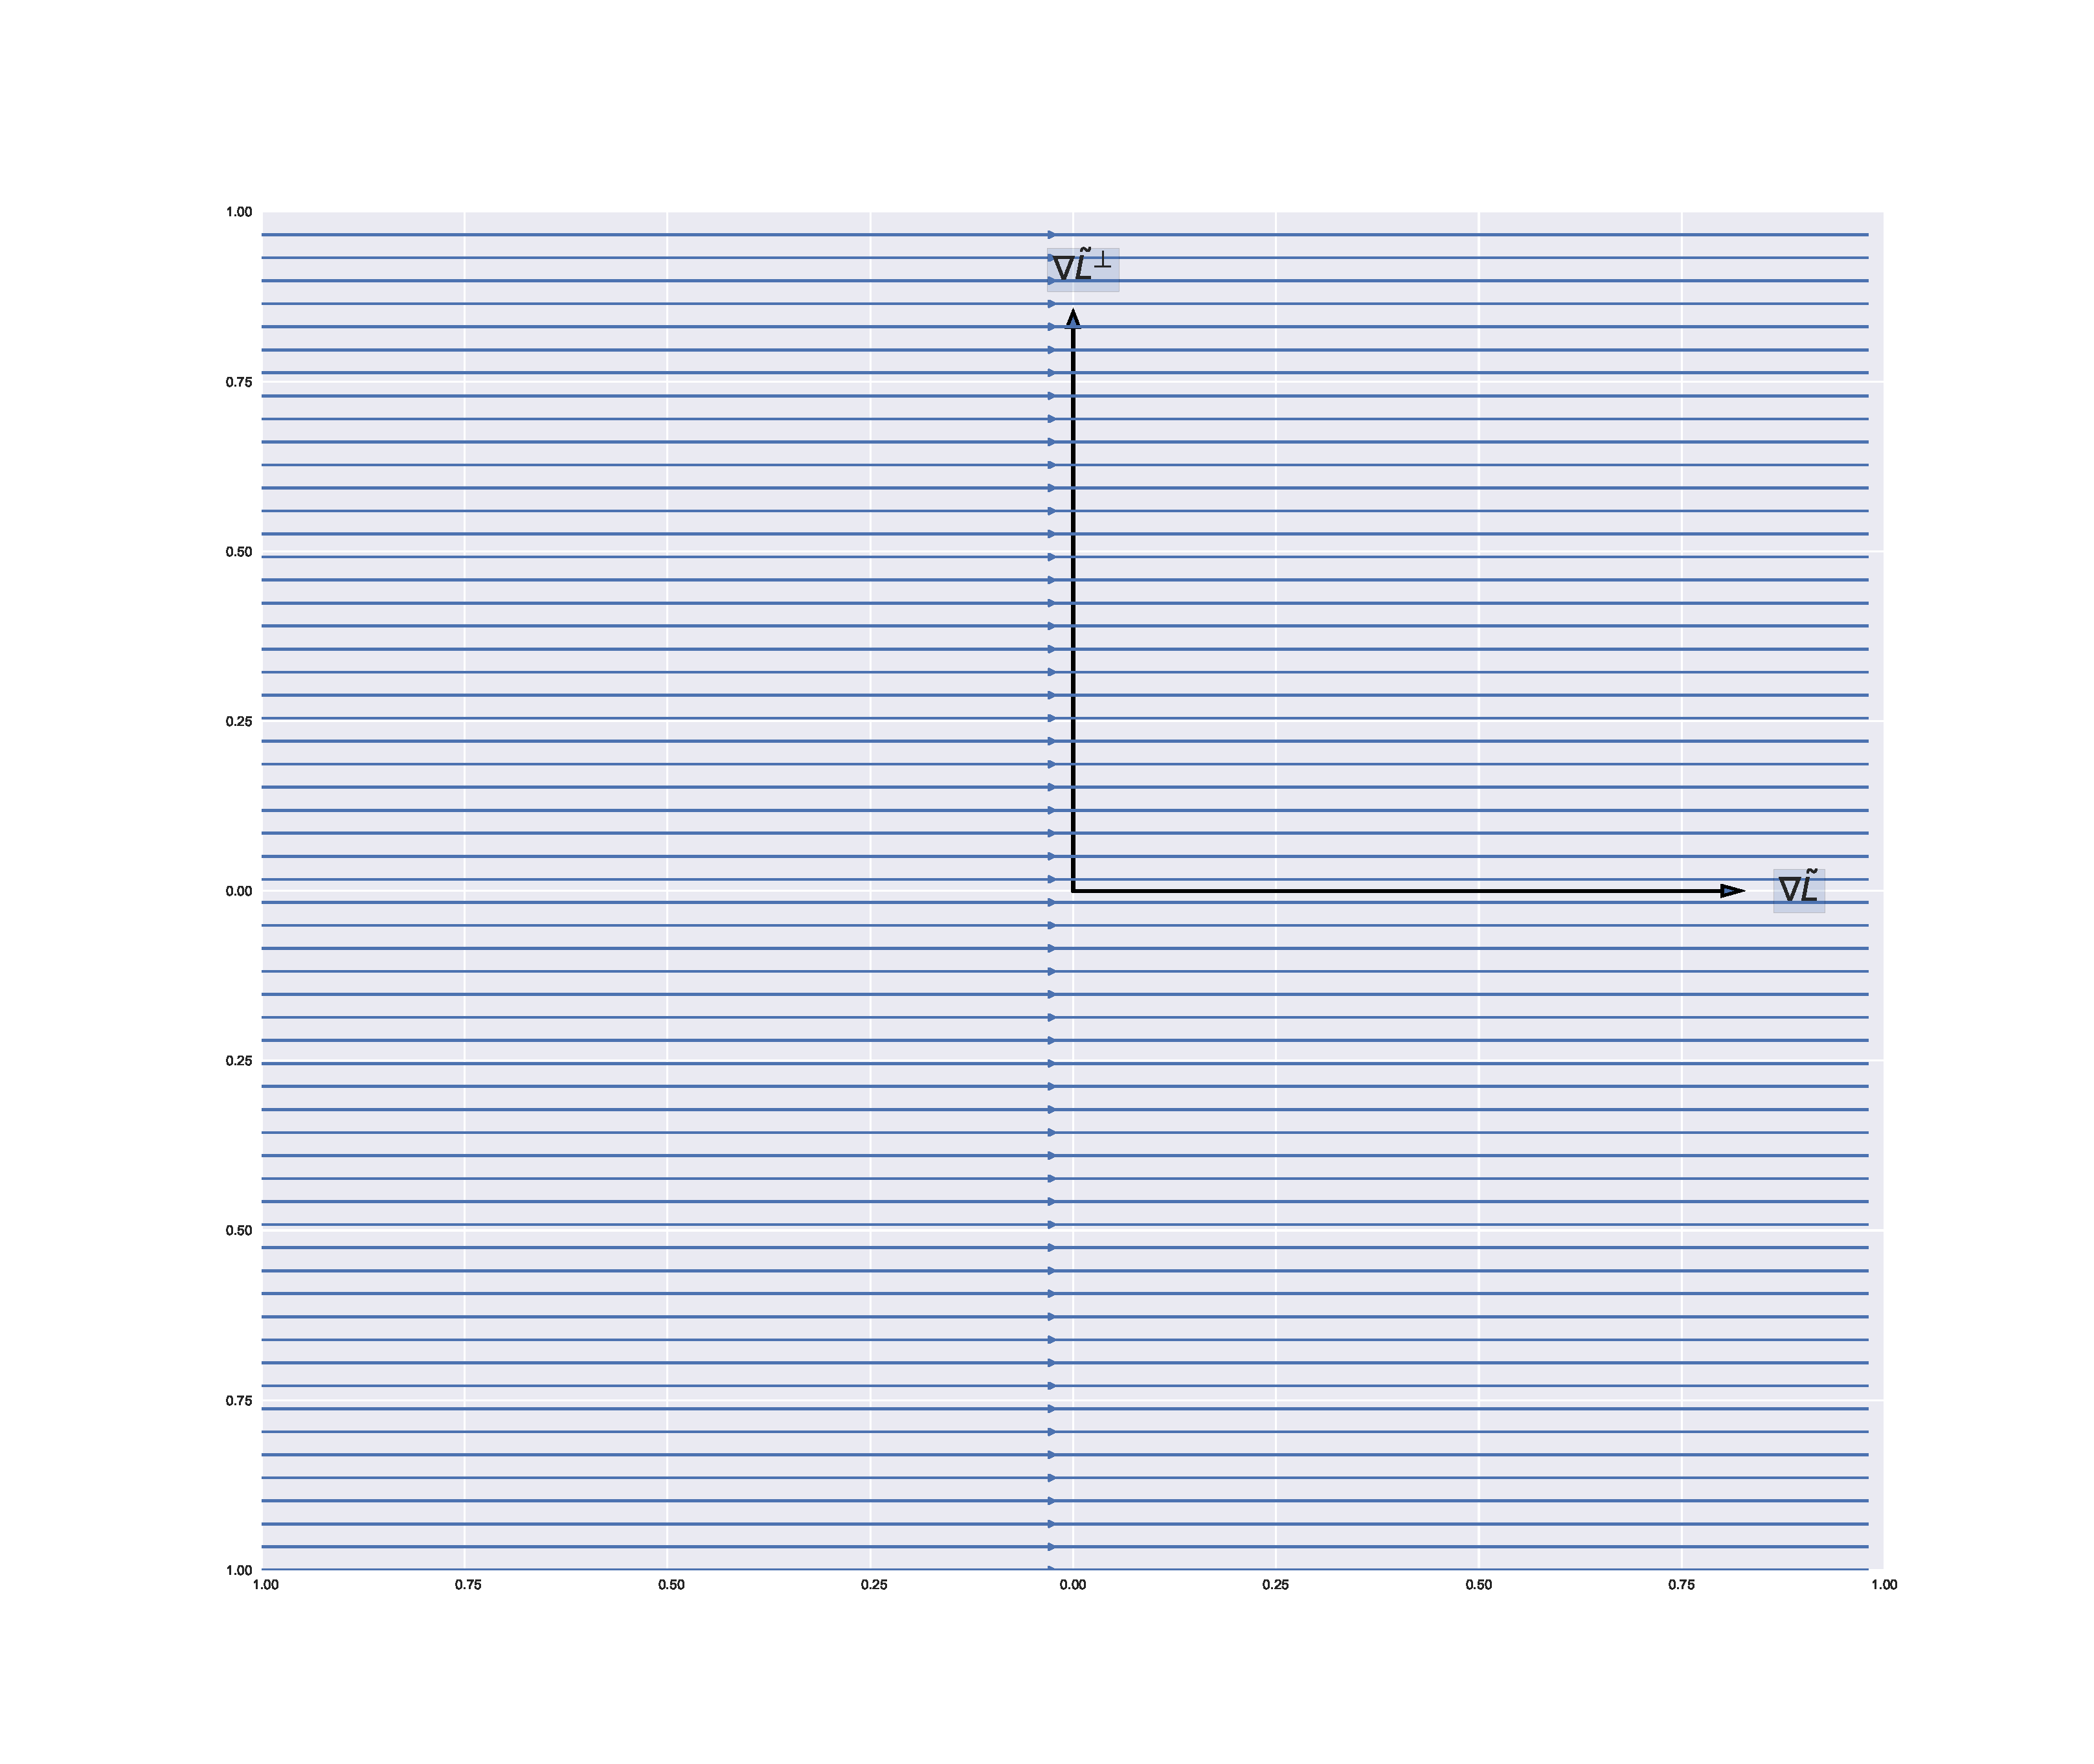
\includegraphics[width=\linewidth]{figures/dynamics_delta_100.pdf}
    \endminipage
    
    \caption{The value of $\delta$ interpolates between different kinds of local trajectories of neurons. The plots are in the coordinate frame $(\nabla \tilde{L}, \nabla \tilde{L}^\bot)$. The left shows $\delta = -100$, in this case, the neurons move radially towards and away from the origin. The middle image shows the trajectories for $\delta = 0$ which has trajectories containing both radial and tangential components. The right image shows the trajectories for $\delta = 100$ which are parallel to the gradient $\nabla \tilde{L}$.}
    \label{fig:my_label}
\end{figure}

\begin{figure}\label{fig:different_funcs_same_init}
    \centering
    \minipage{0.33\textwidth}
    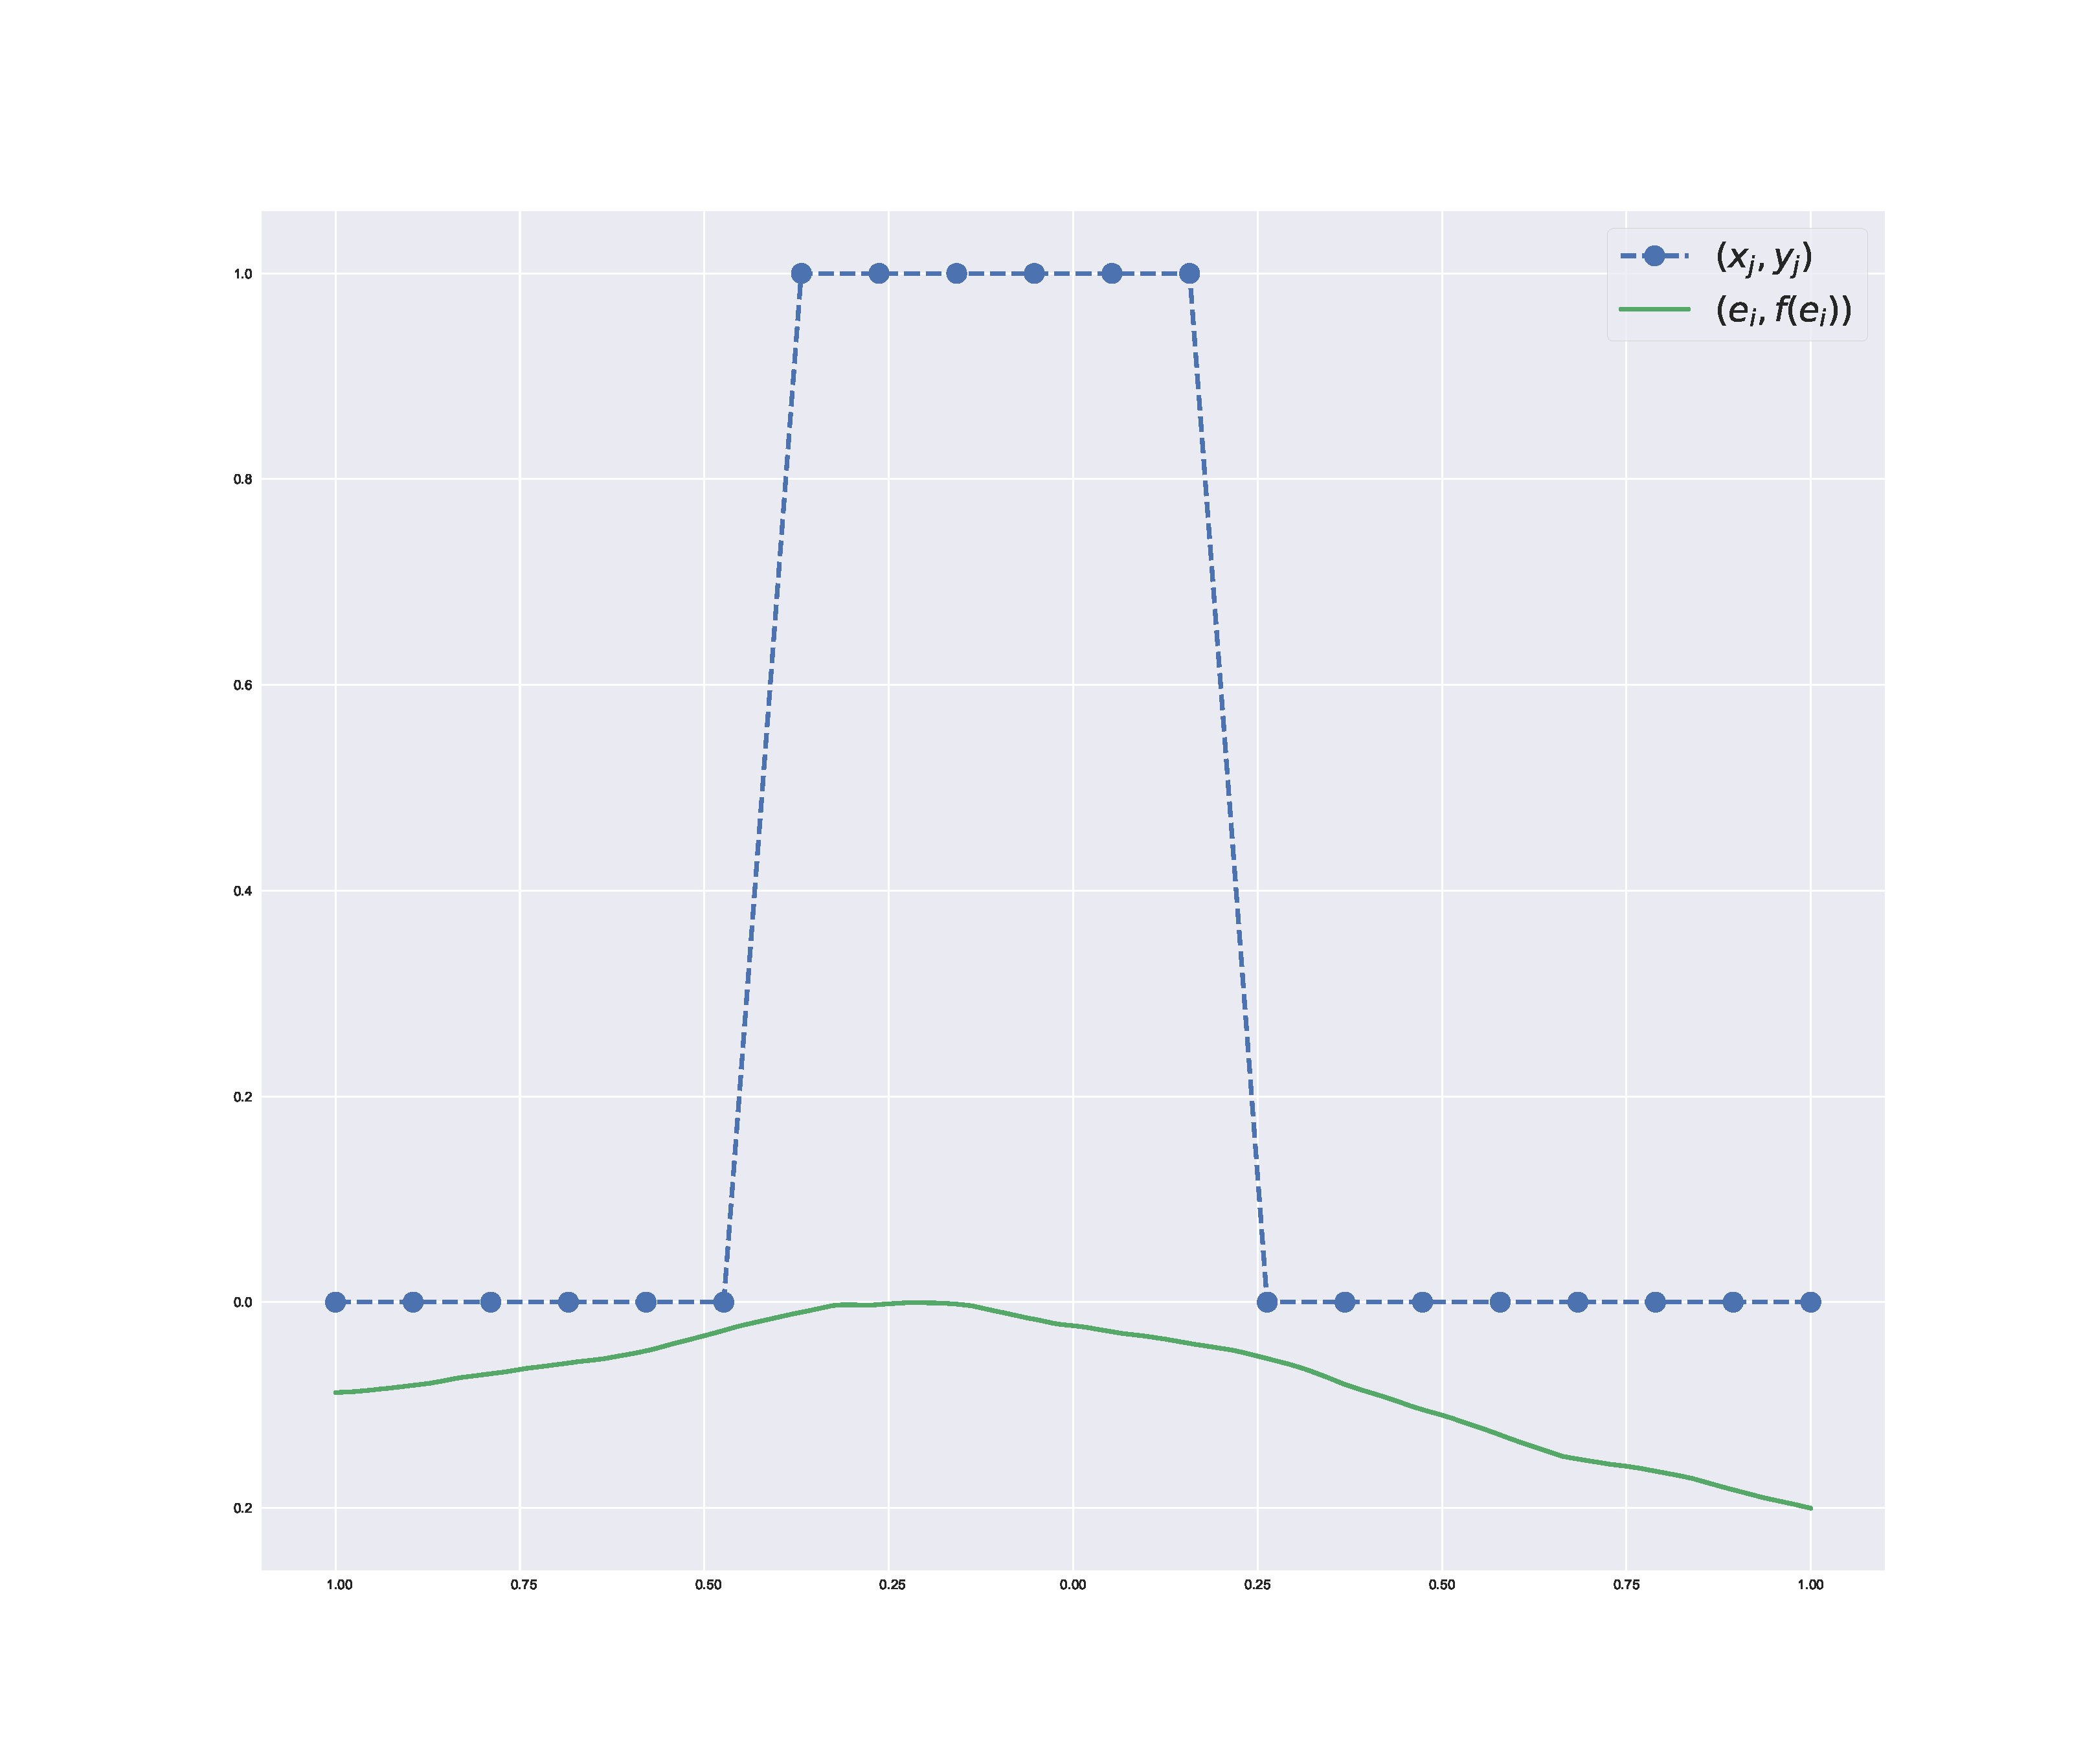
\includegraphics[width=\linewidth]{figures/same_init_different_func_square_init.pdf}
    \endminipage\hfill
    % \minipage{0.2\textwidth}
    % 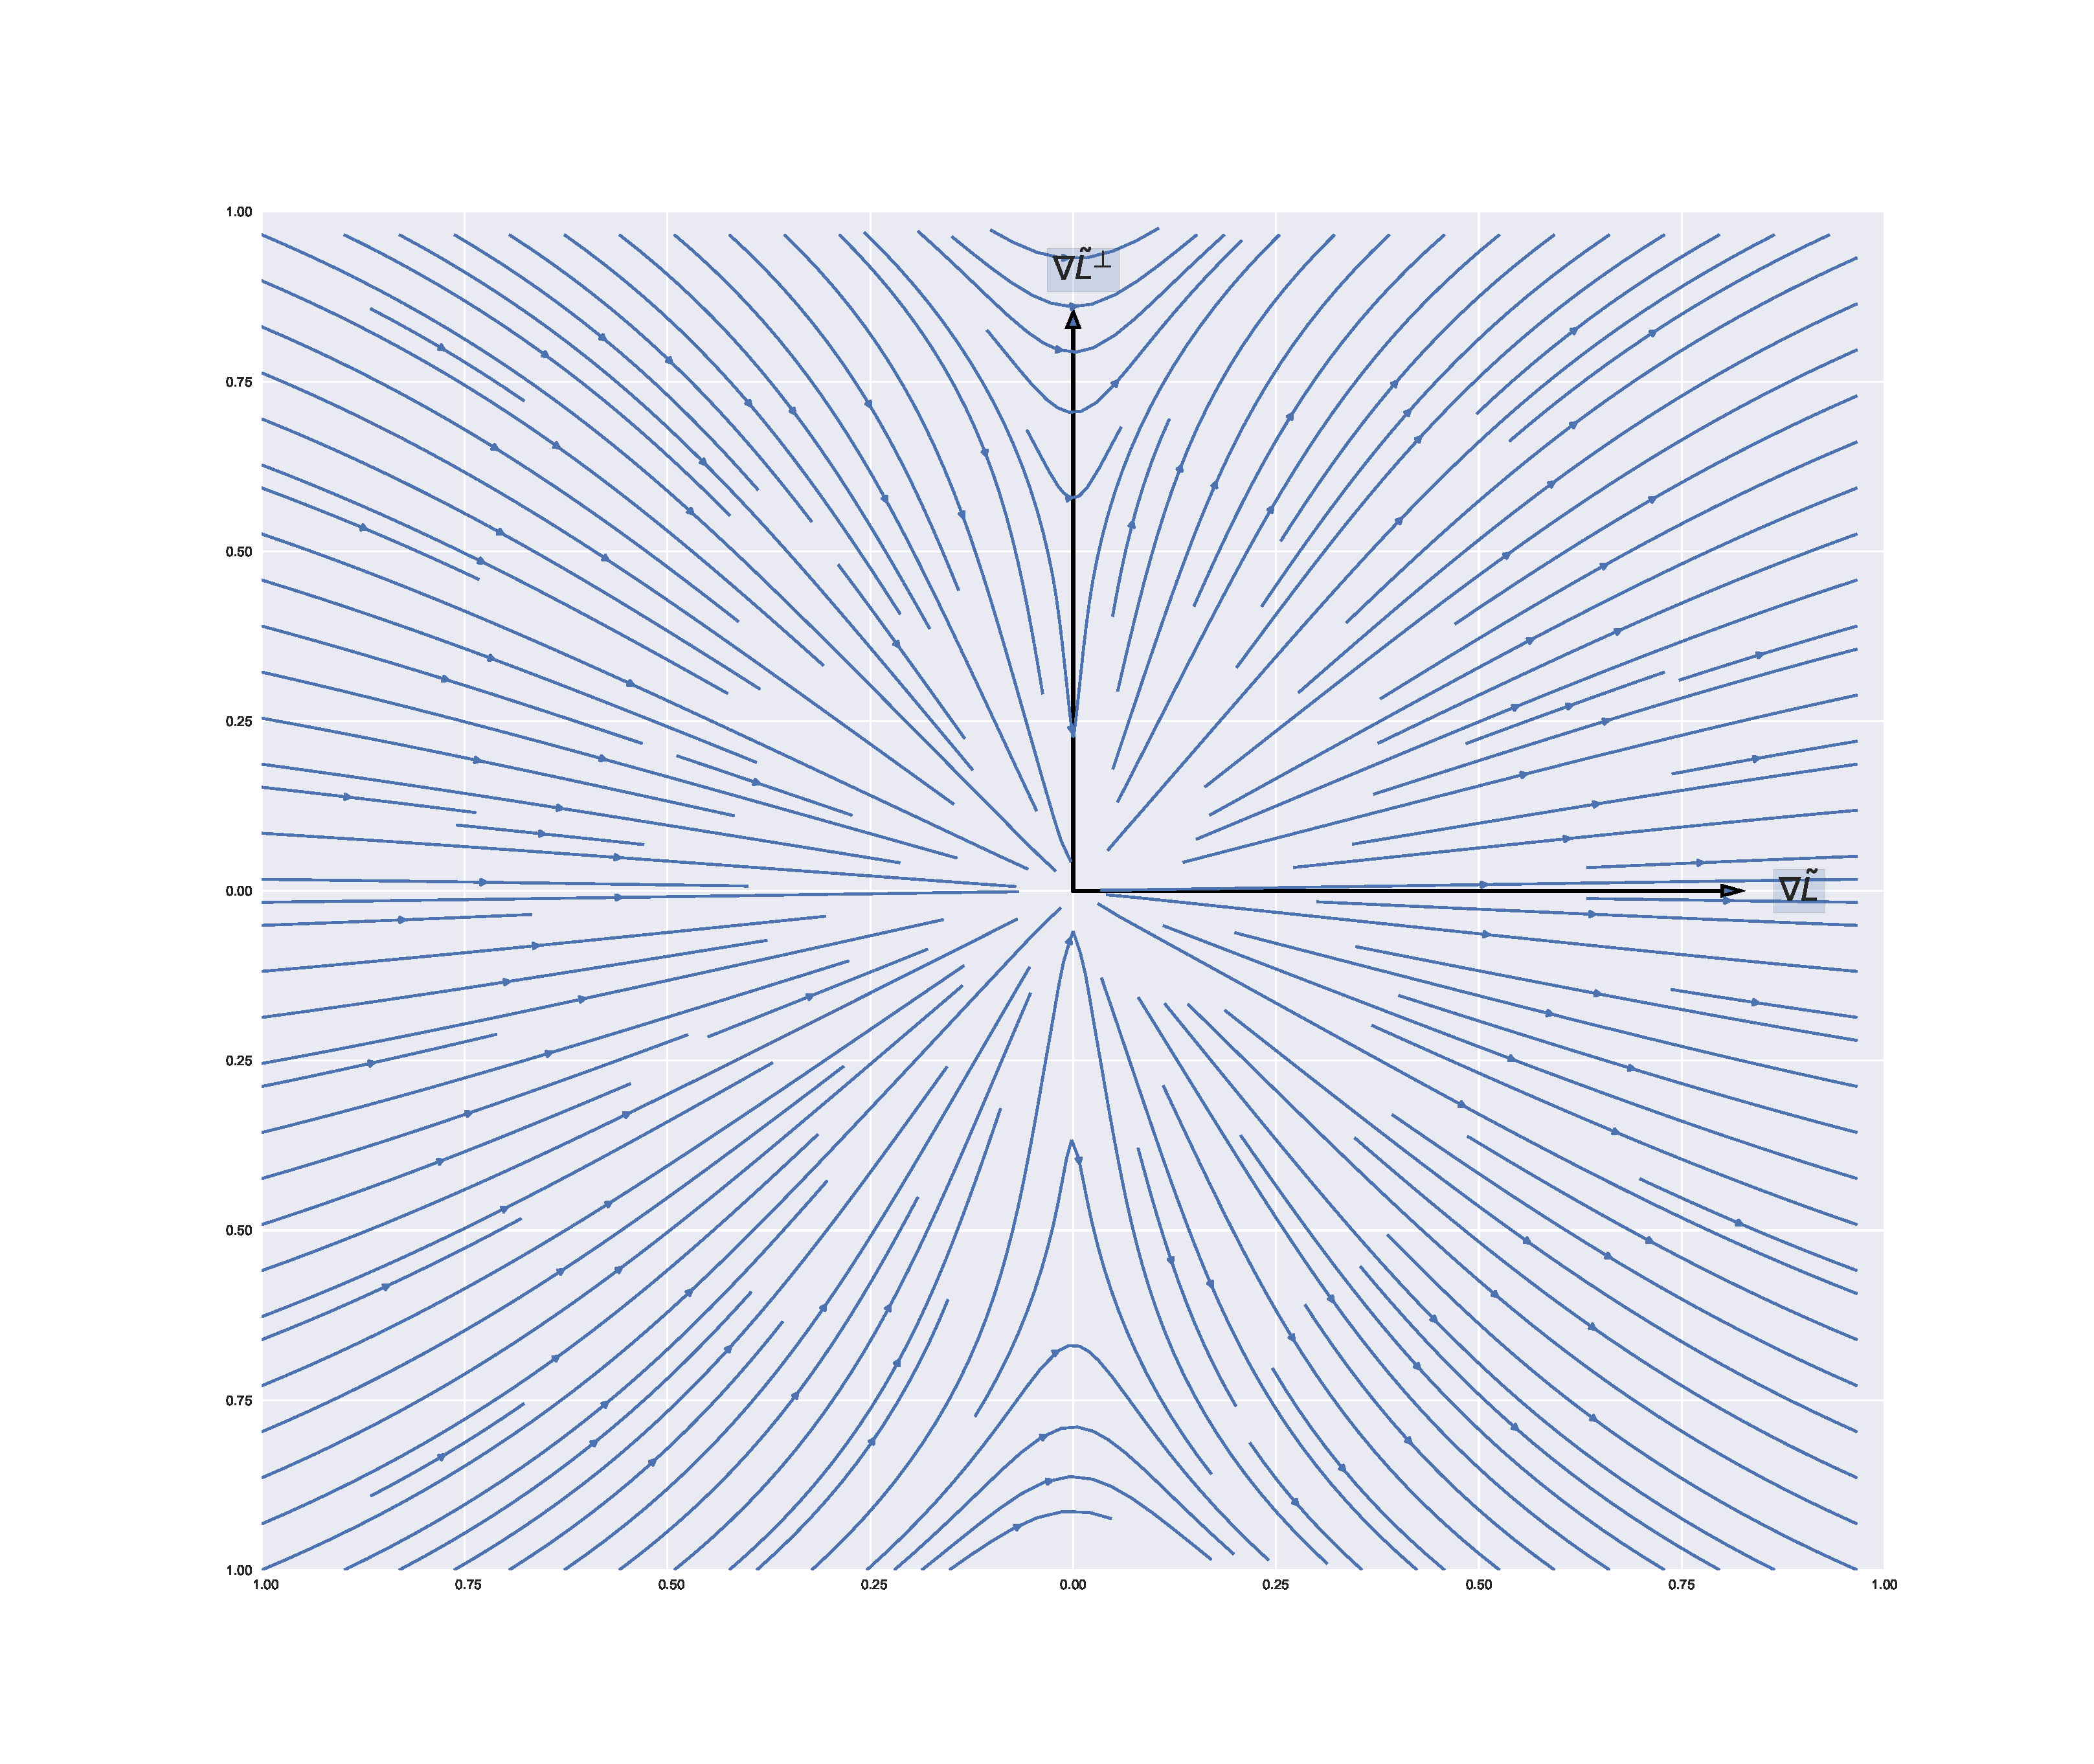
\includegraphics[width=\linewidth]{figures/dynamics_delta_-1.pdf}
    % \endminipage\hfill
    \minipage{0.33\textwidth}
    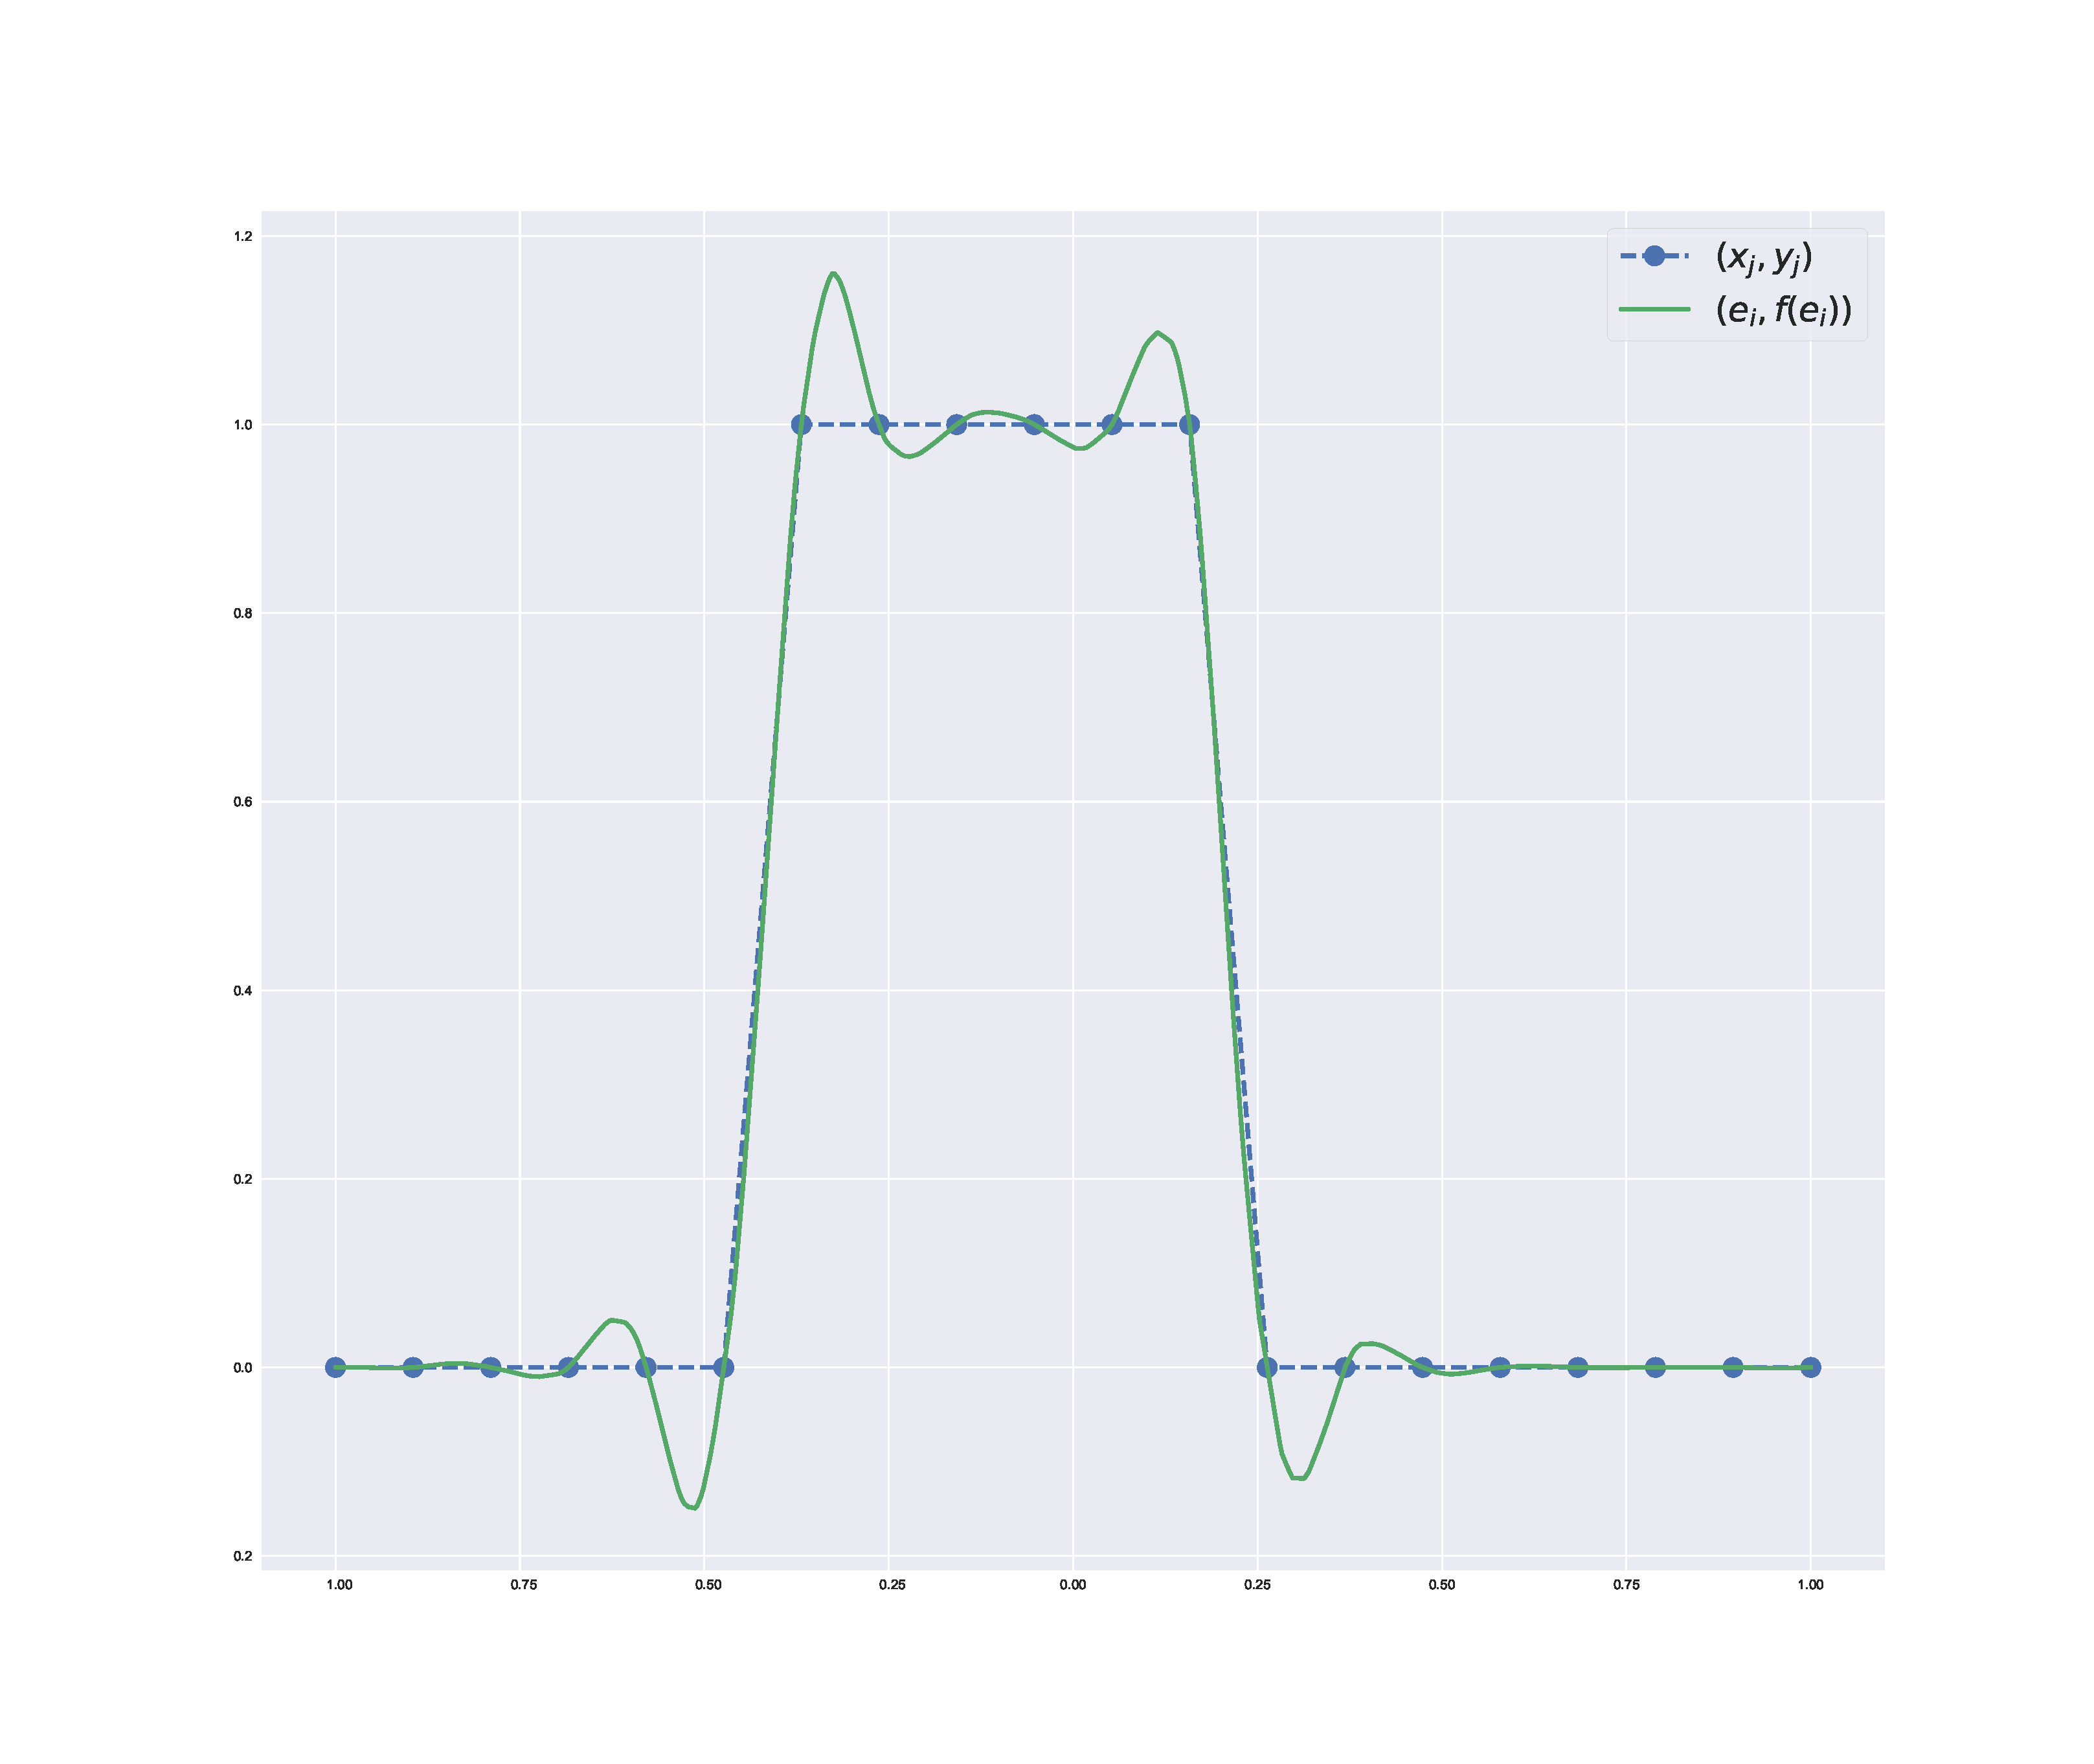
\includegraphics[width=\linewidth]{figures/same_init_different_func_square_1.pdf}
    \endminipage\hfill
    % \minipage{0.2\textwidth}
    % 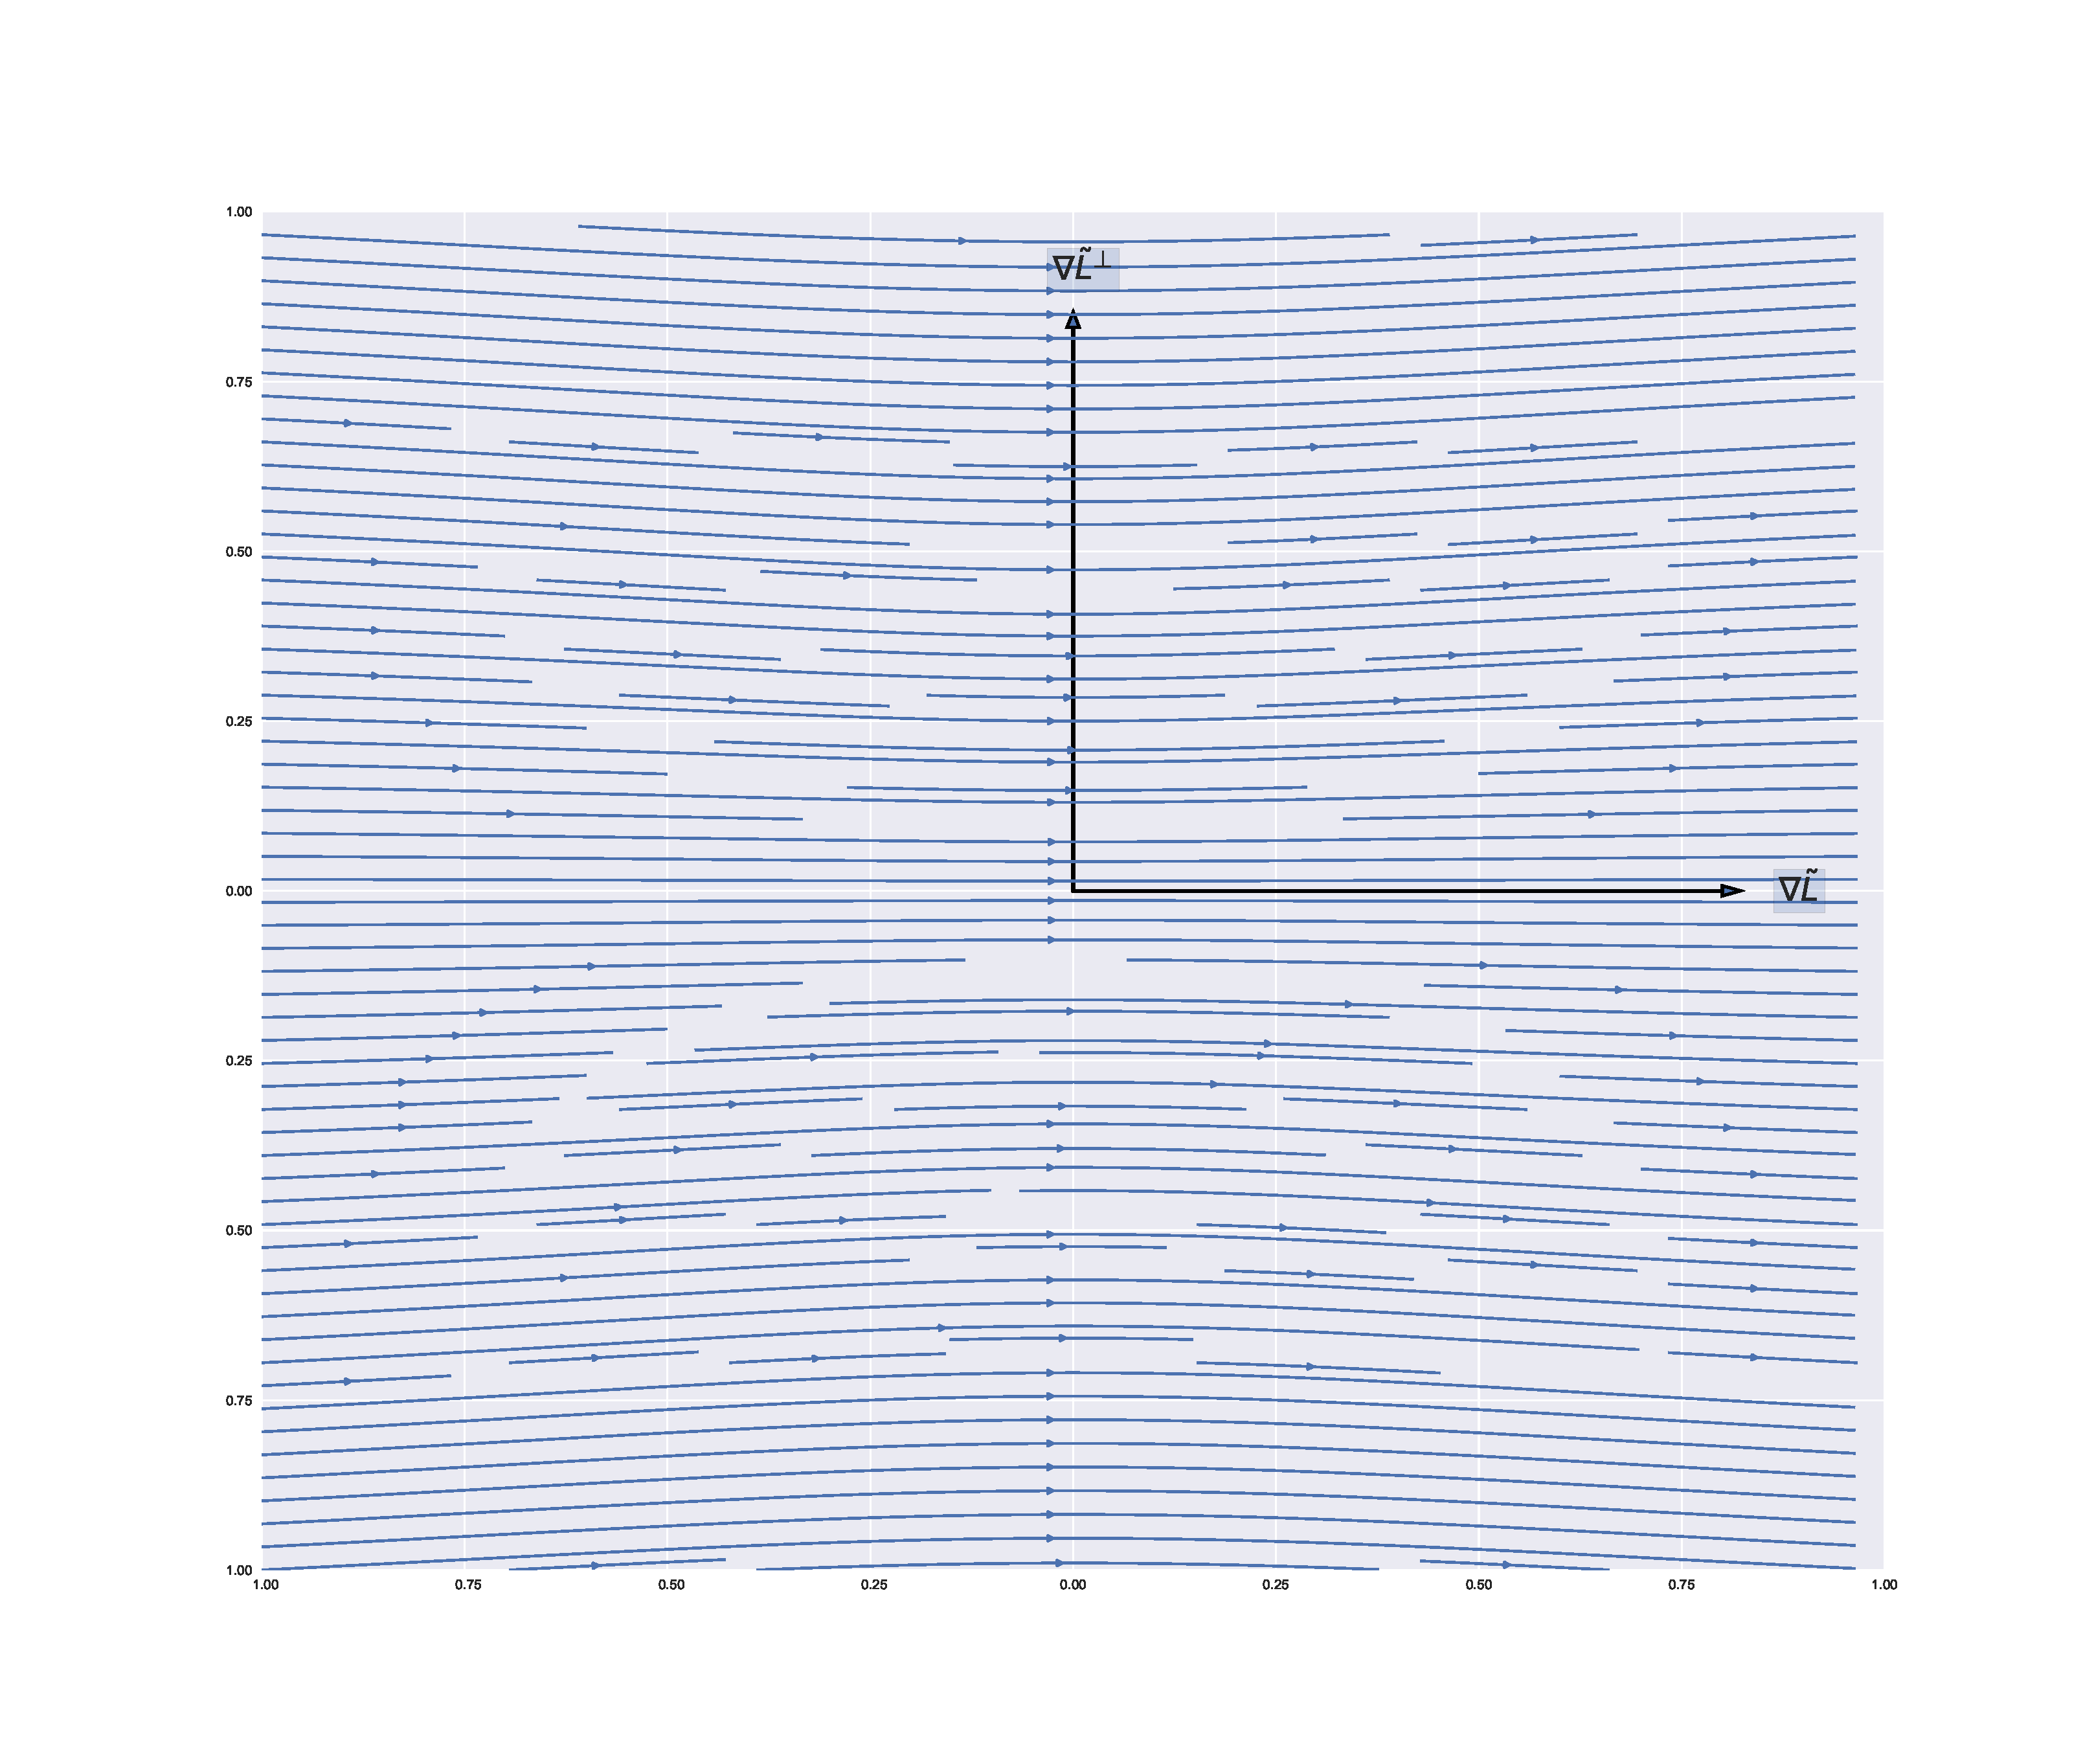
\includegraphics[width=\linewidth]{figures/dynamics_delta_1.pdf}
    % \endminipage\hfill
    \minipage{0.33\textwidth}
    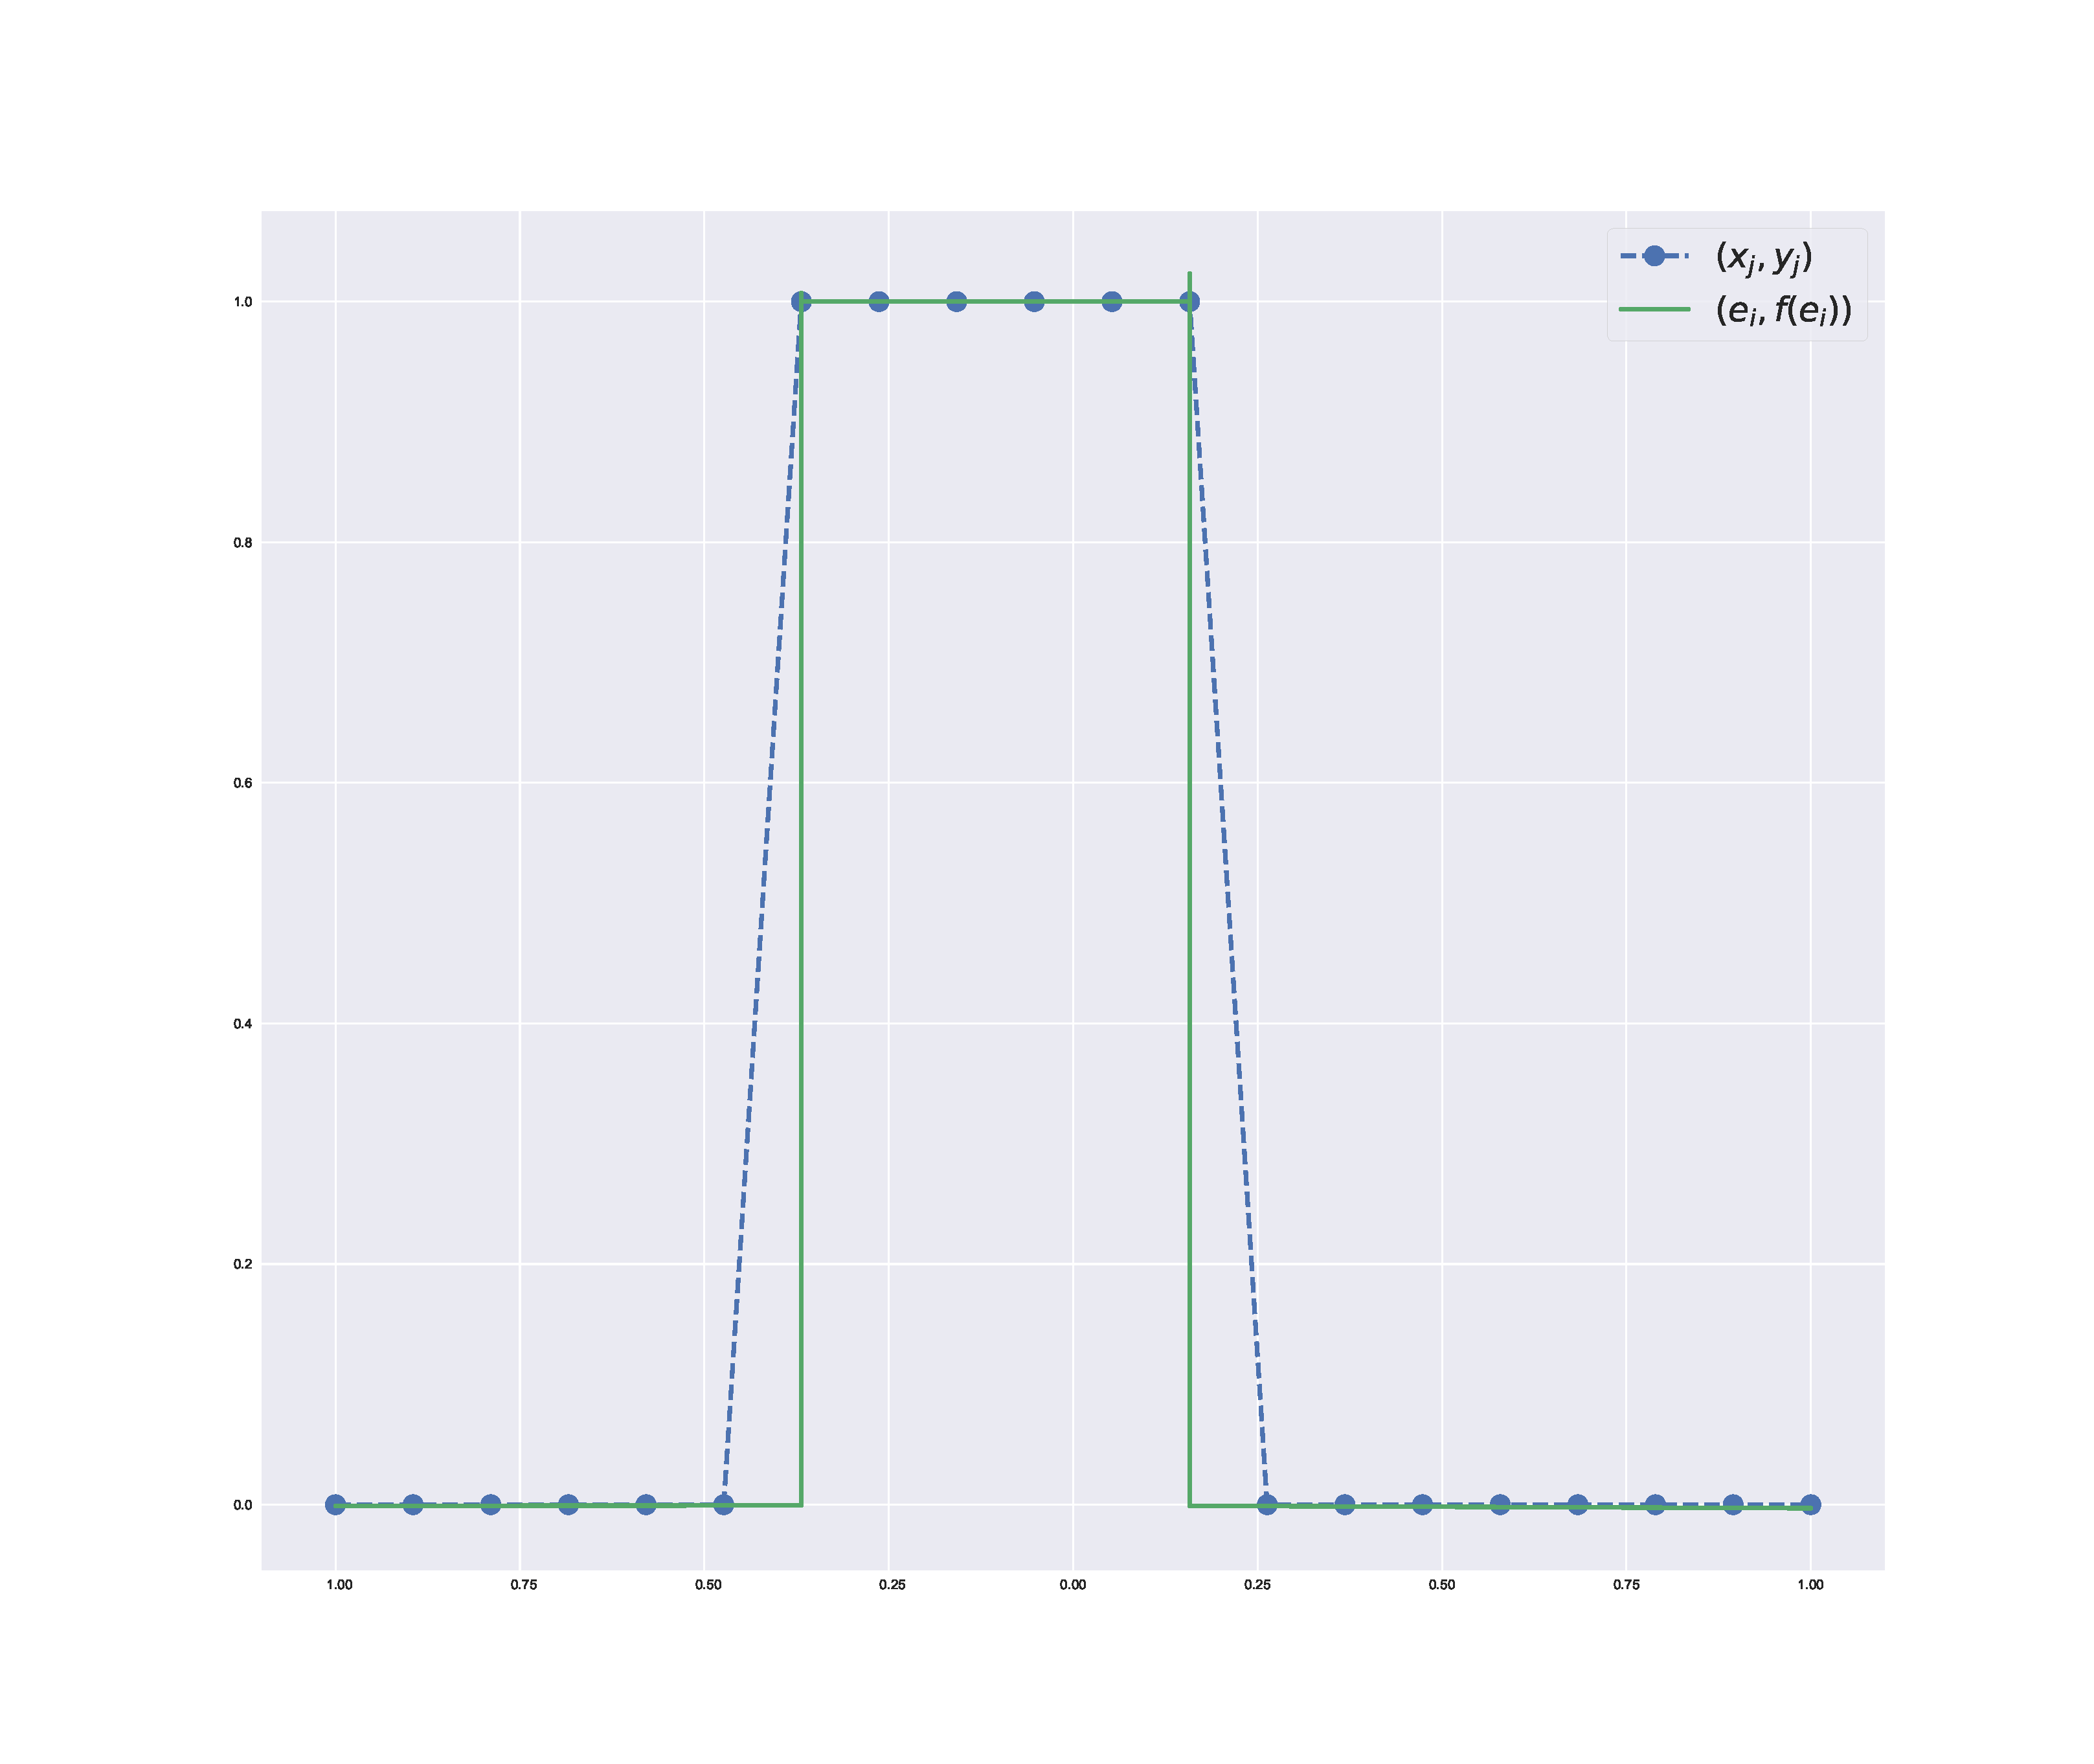
\includegraphics[width=\linewidth]{figures/same_init_different_func_square_1000.pdf}
    \endminipage
    
    \caption{The same initial function can yield very different results: the left image is the initial function for the two right ones. The initial parameters ($\bm a, \bm b, \bm c$) were the same as those in the middle image but scaled by a factor of 1000, 1000 and 0.001 respectively}
\end{figure}

% \begin{itemize}
%     \item If $c_i^2 \ll (a_i^2 + b_i^2)$, which means that $\delta <
%     0$, then $\xi_i'(t) \propto (u(t),v(t))$, and the reduced neuron
%     moves~\emph{radially} (\todo{Figure \ref{fig:todo}}).
%     \item If $c_i^2 \gg (a_i^2 + b_i^2)$, which means that $\delta > 0$, then
%     $\xi_i'(t) \propto \nabla \tilde L(\xi)_i$, so the reduced neuron follows the gradient field $\nabla \tilde{L}$ (\todo{Figure \ref{fig:todo}}).
% \end{itemize}


% The shapes of a neuron's trajectory is thus controlled by the invariant $\delta_i$ which can be altered by re-scaling the gradient flow (changing $\alpha$ or $\beta$), or changing the initial distribution from which the parameters $\theta = (a, b, c)$ are sampled. 




\begin{remark}
\note{Discuss relationship with asymptotics of other works.}
\end{remark}

If $\rho_i \ll |\delta_i|$ holds for all neurons, then we say that we are in the regime of \emph{kernel learning}; similarly if $\rho_i \gg |\delta_i|$ holds for all neurons we are in the regime of \emph{purely adaptive learning}. In the next section, we study the dynamics in these two extreme regimes.
In particular, we study how the two extrema above bias the network to very different kinds of solutions: kernel learning motion biases towards smooth solutions, while purely adaptive learning biases towards piecewise linear solutions. 

\begin{remark}
The kernel and purely adaptive regimes are related to the kernel dynamics \eqref{eq:tangent_kernel}. Kernel Learning corresponds to the function only evolving along $\bm K^c$ and Adaptive Learning corresponds to evolution along $\bm K^{ab}$.  
\end{remark}










\subsection{Kernel Learning}
We first consider the regime of kernel learning, where $\delta_i \ll -\|\xi_i\|$. In this regime, reduced neurons move radially away from the origin (see Figure \ref{fig:trajectories}). These trajectories are equivalent to training only the outer-layer parameters ($\bm c$) while keeping the inner-layer parameters ($\bm a, \bm b$) fixed. In the overparameterized case, this corresponds to the least squares problem
\begin{equation}\label{eq:least_squares_op}
    \text{minimize } \|\bm c\|^2 \text{ s.t. } f_{\bm \theta}(x) = \bm M_{ab} \bm c = \bm y
\end{equation}

Solutions $f(x)$ can be written in terms of the kernel (\todo{see supplemental sections ...})
\begin{equation}
\begin{gathered}
    f(x) = \sum_{j=1}^s \alpha_j K(x_j, x) \text{ where } \\
    K(x, x') = \sum_{i=1}^m [a_i x + b_i]_+ [a_i x' + b_i]_+ \text{ and } \alpha_j = (\bm K_c^{-1} \bm y)_j  
\end{gathered}
\end{equation}

Note that $K(x_i, x_j) = \bm K_{c, ij}$. Also note that gradient flow will converge to this solution only if $\bm c(0)$ is initialized sufficiently close to the origin. To understand solutions to \eqref{eq:least_squares_op}, we consider the $K$ as an approximation of the the network in the limit as the number of neurons goes to infinity ($m \rightarrow \infty$). In this case, the parameters $\bm \theta_i$ become functions $\bm \theta(s)$. Assuming the domain of $f$ is $[k_1, k_2]$, as $m \rightarrow \infty$ we have that

\begin{equation}
    K(x, x') = \int_{k_1}^{k_2} [a(s)x + b(s)]_+ [a(s)x' + b(s)]_+ ds
\end{equation}

\begin{lemma}\label{le:curvature_minimizer}
In this infinite width limit ($m = \infty$), $c(s) = \partial_x^2 f(x)$
\end{lemma}

Thus solutions to the least squares problem \eqref{eq:least_squares_op} minimize \emph{curvature} subject to equality constraints. 
\begin{lemma}\label{le:cubic_poly}
When $m = \infty$ and $\bm \theta(s) ~ \lambda U(-1, 1)$ are initialized from a uniform distribution, then the function $K(x, x')$ is a cubic polynomial in $x$ and $x'$.
\end{lemma}

We remark that machine learning packages such as PyTorch use a uniform distribution for linear layer parameter initialization by default.

\begin{corollary}
A corollary of Lemmas~\ref{le:curvature_minimizer}~and~\ref{le:cubic_poly} are that solutions to the gradient flow with $\|c(0)\| = 0$ are cubic splines. 
\end{corollary}

We verify that indeed, solutions to \eqref{eq:leastsquares} converge to cubic splines as $m$ grows in Figure~\ref{fig:cubic_splines}. We also point out that in Kernel Learning, early termination of gradient flow acts as a regularizer favoring smooth, non-interpolatory solutions (see \cite{NTKJacot} and \todo{Section~\ref{sec:todo}} of the supplementary).



\subsection{Purely Adaptive Learning}
We now consider the Purely Adaptive regime where $\delta_i \ll \| \xi_i \|$. In this regime, neurons move parallel to the reduced gradient field $\nabla \tilde{L}(\bm \xi)$ (see Figure \ref{fig:trajectories}). These trajectories are equivalent to those when training only the bottom layer parameters $(\bm a, \bm b)$ while keeping the top layer ($\bm c$) fixed. To understand the dynamics in this regime, we write the function $f$ in terms of the reduced parameters

\begin{equation}
    f_{\bm \xi}(x) = \sum_{i=1}^m \langle (x, 1), (u_i, v_i) \rangle_+ 
\end{equation}

The gradient of the loss with respect to the reduced parameters is 
\begin{equation}\label{eq:grad_reduced}
    \nabla \tilde{L}(\bm \xi)_i = \sum_{i=1}^s (f_{\bm \xi}(x_j) - y_j) \epsilon_i \tau_{ij} \begin{bmatrix}x_j \\ 1\end{bmatrix} 
\end{equation}

\begin{figure}
    \centering
    \minipage{0.33\textwidth}
        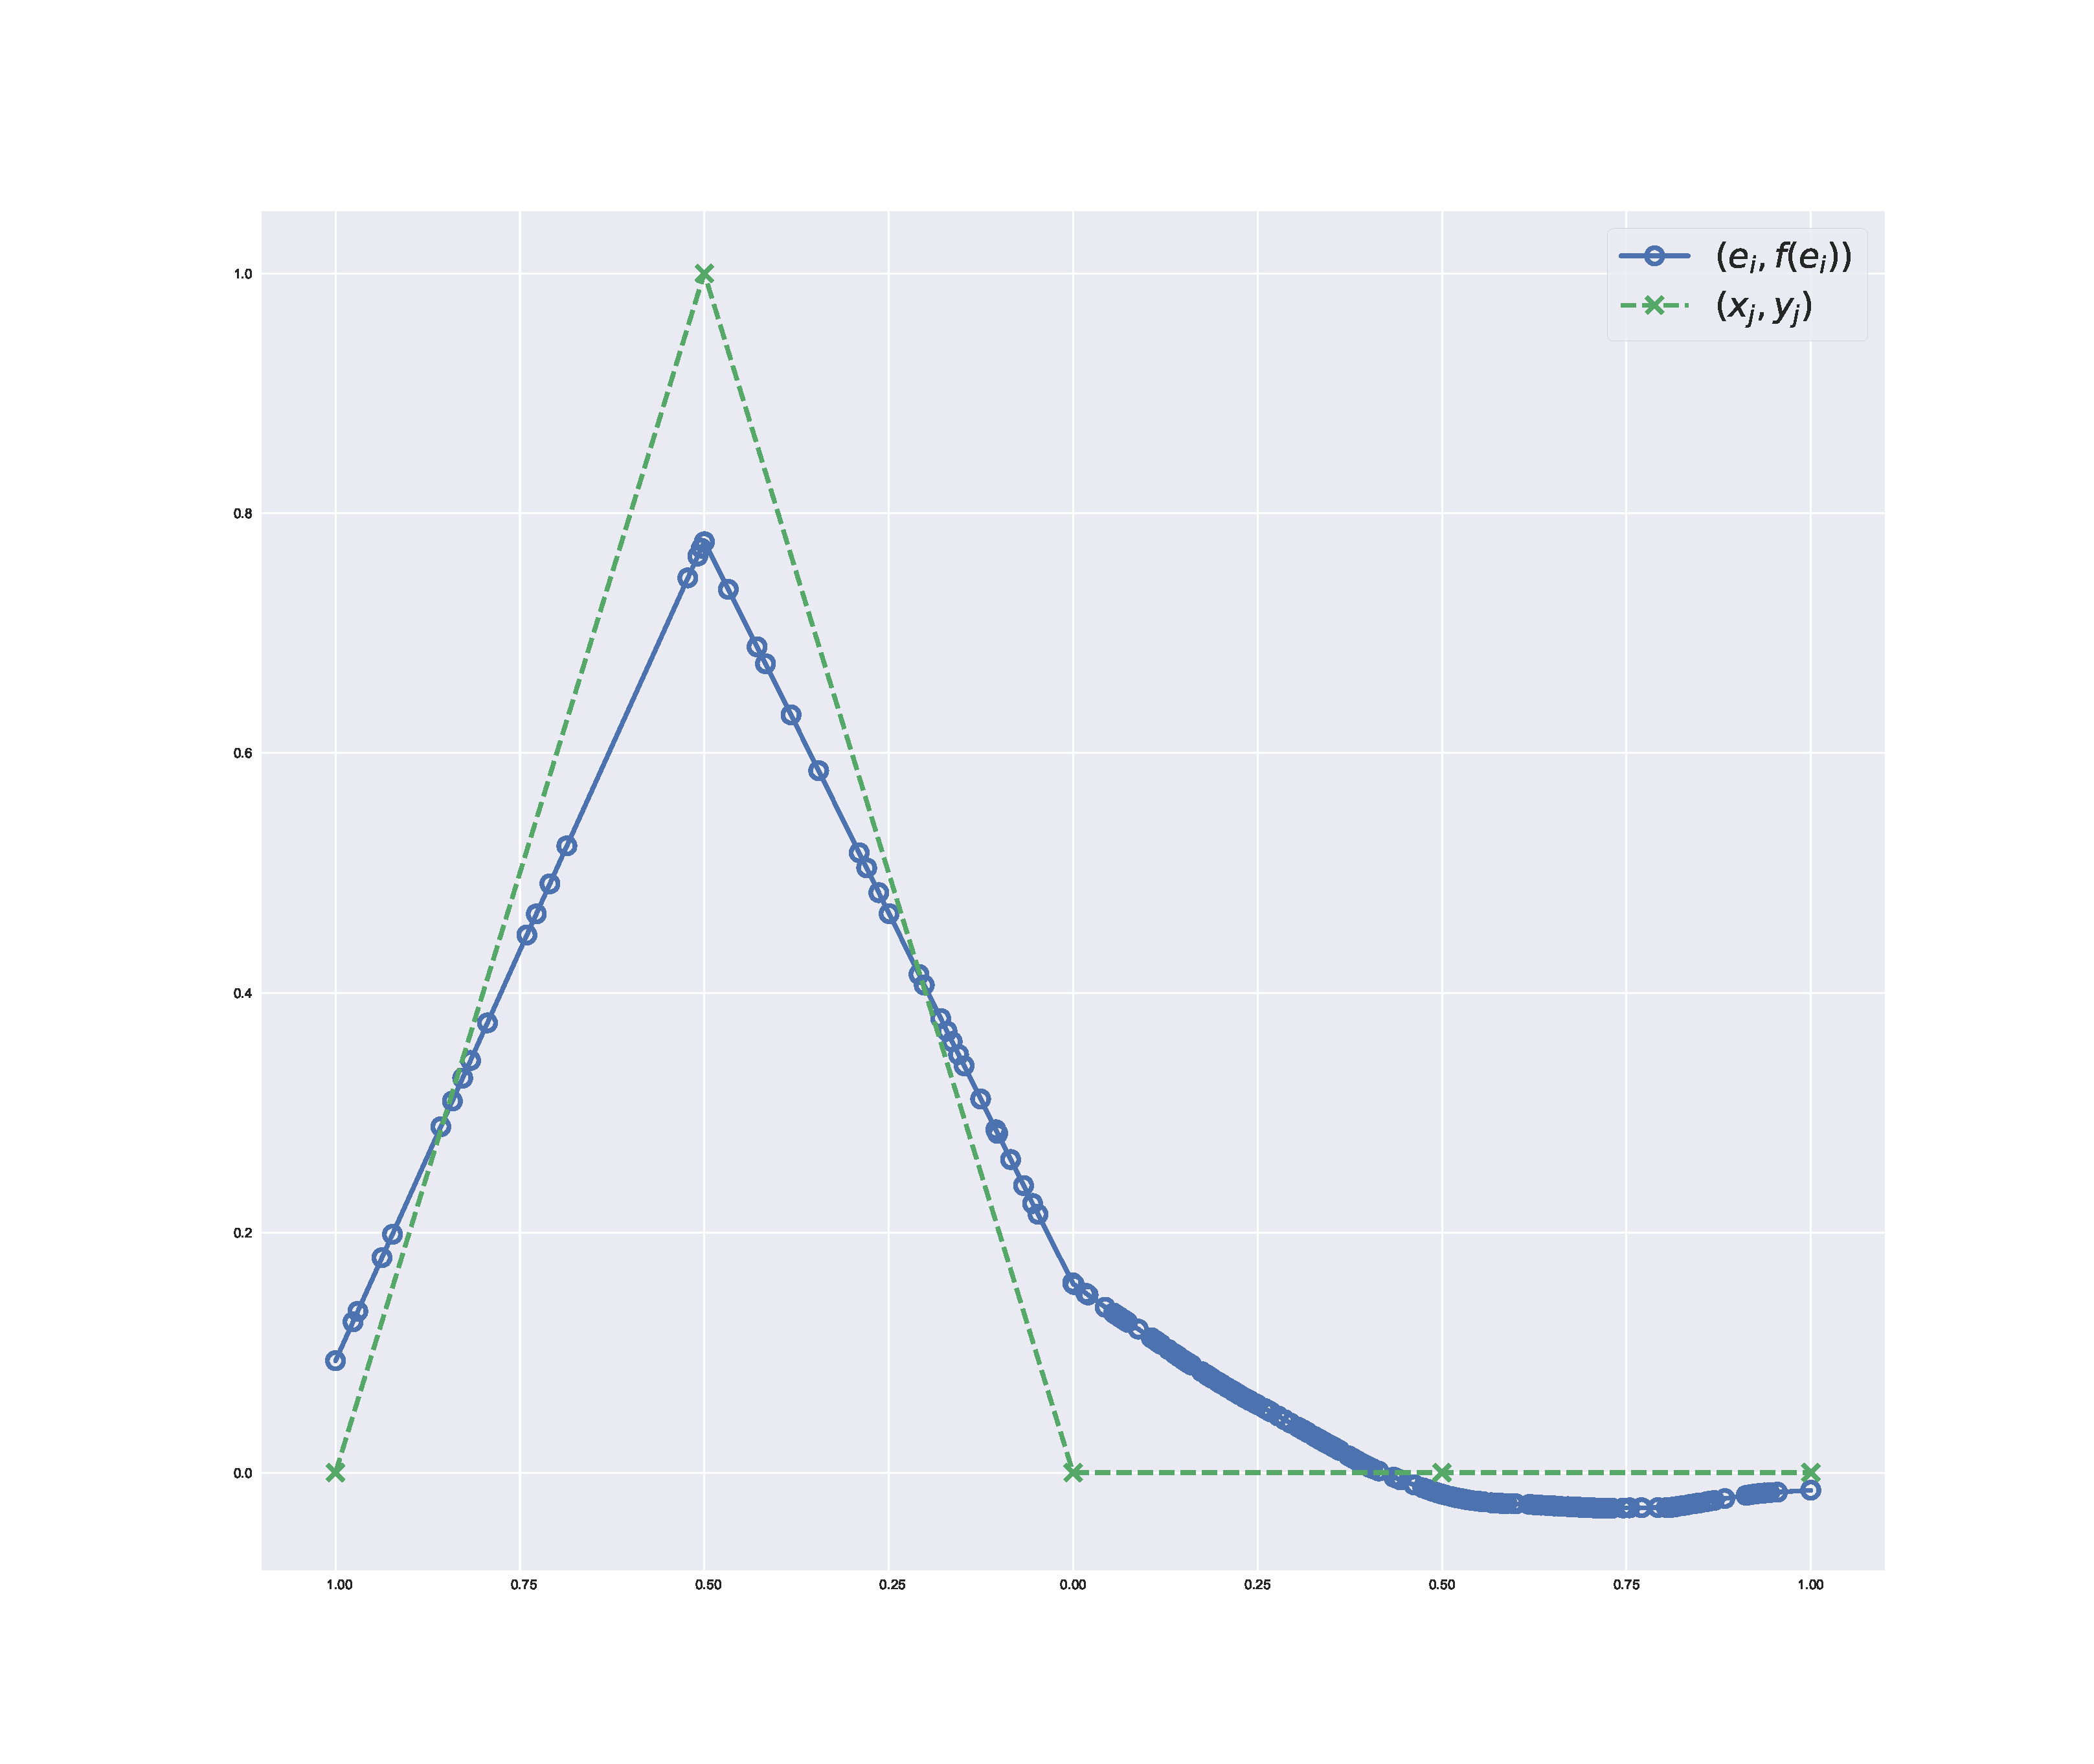
\includegraphics[width=\linewidth]{figures/reduced_gradient_recon.pdf}
    \endminipage
    \minipage{0.33\textwidth}
        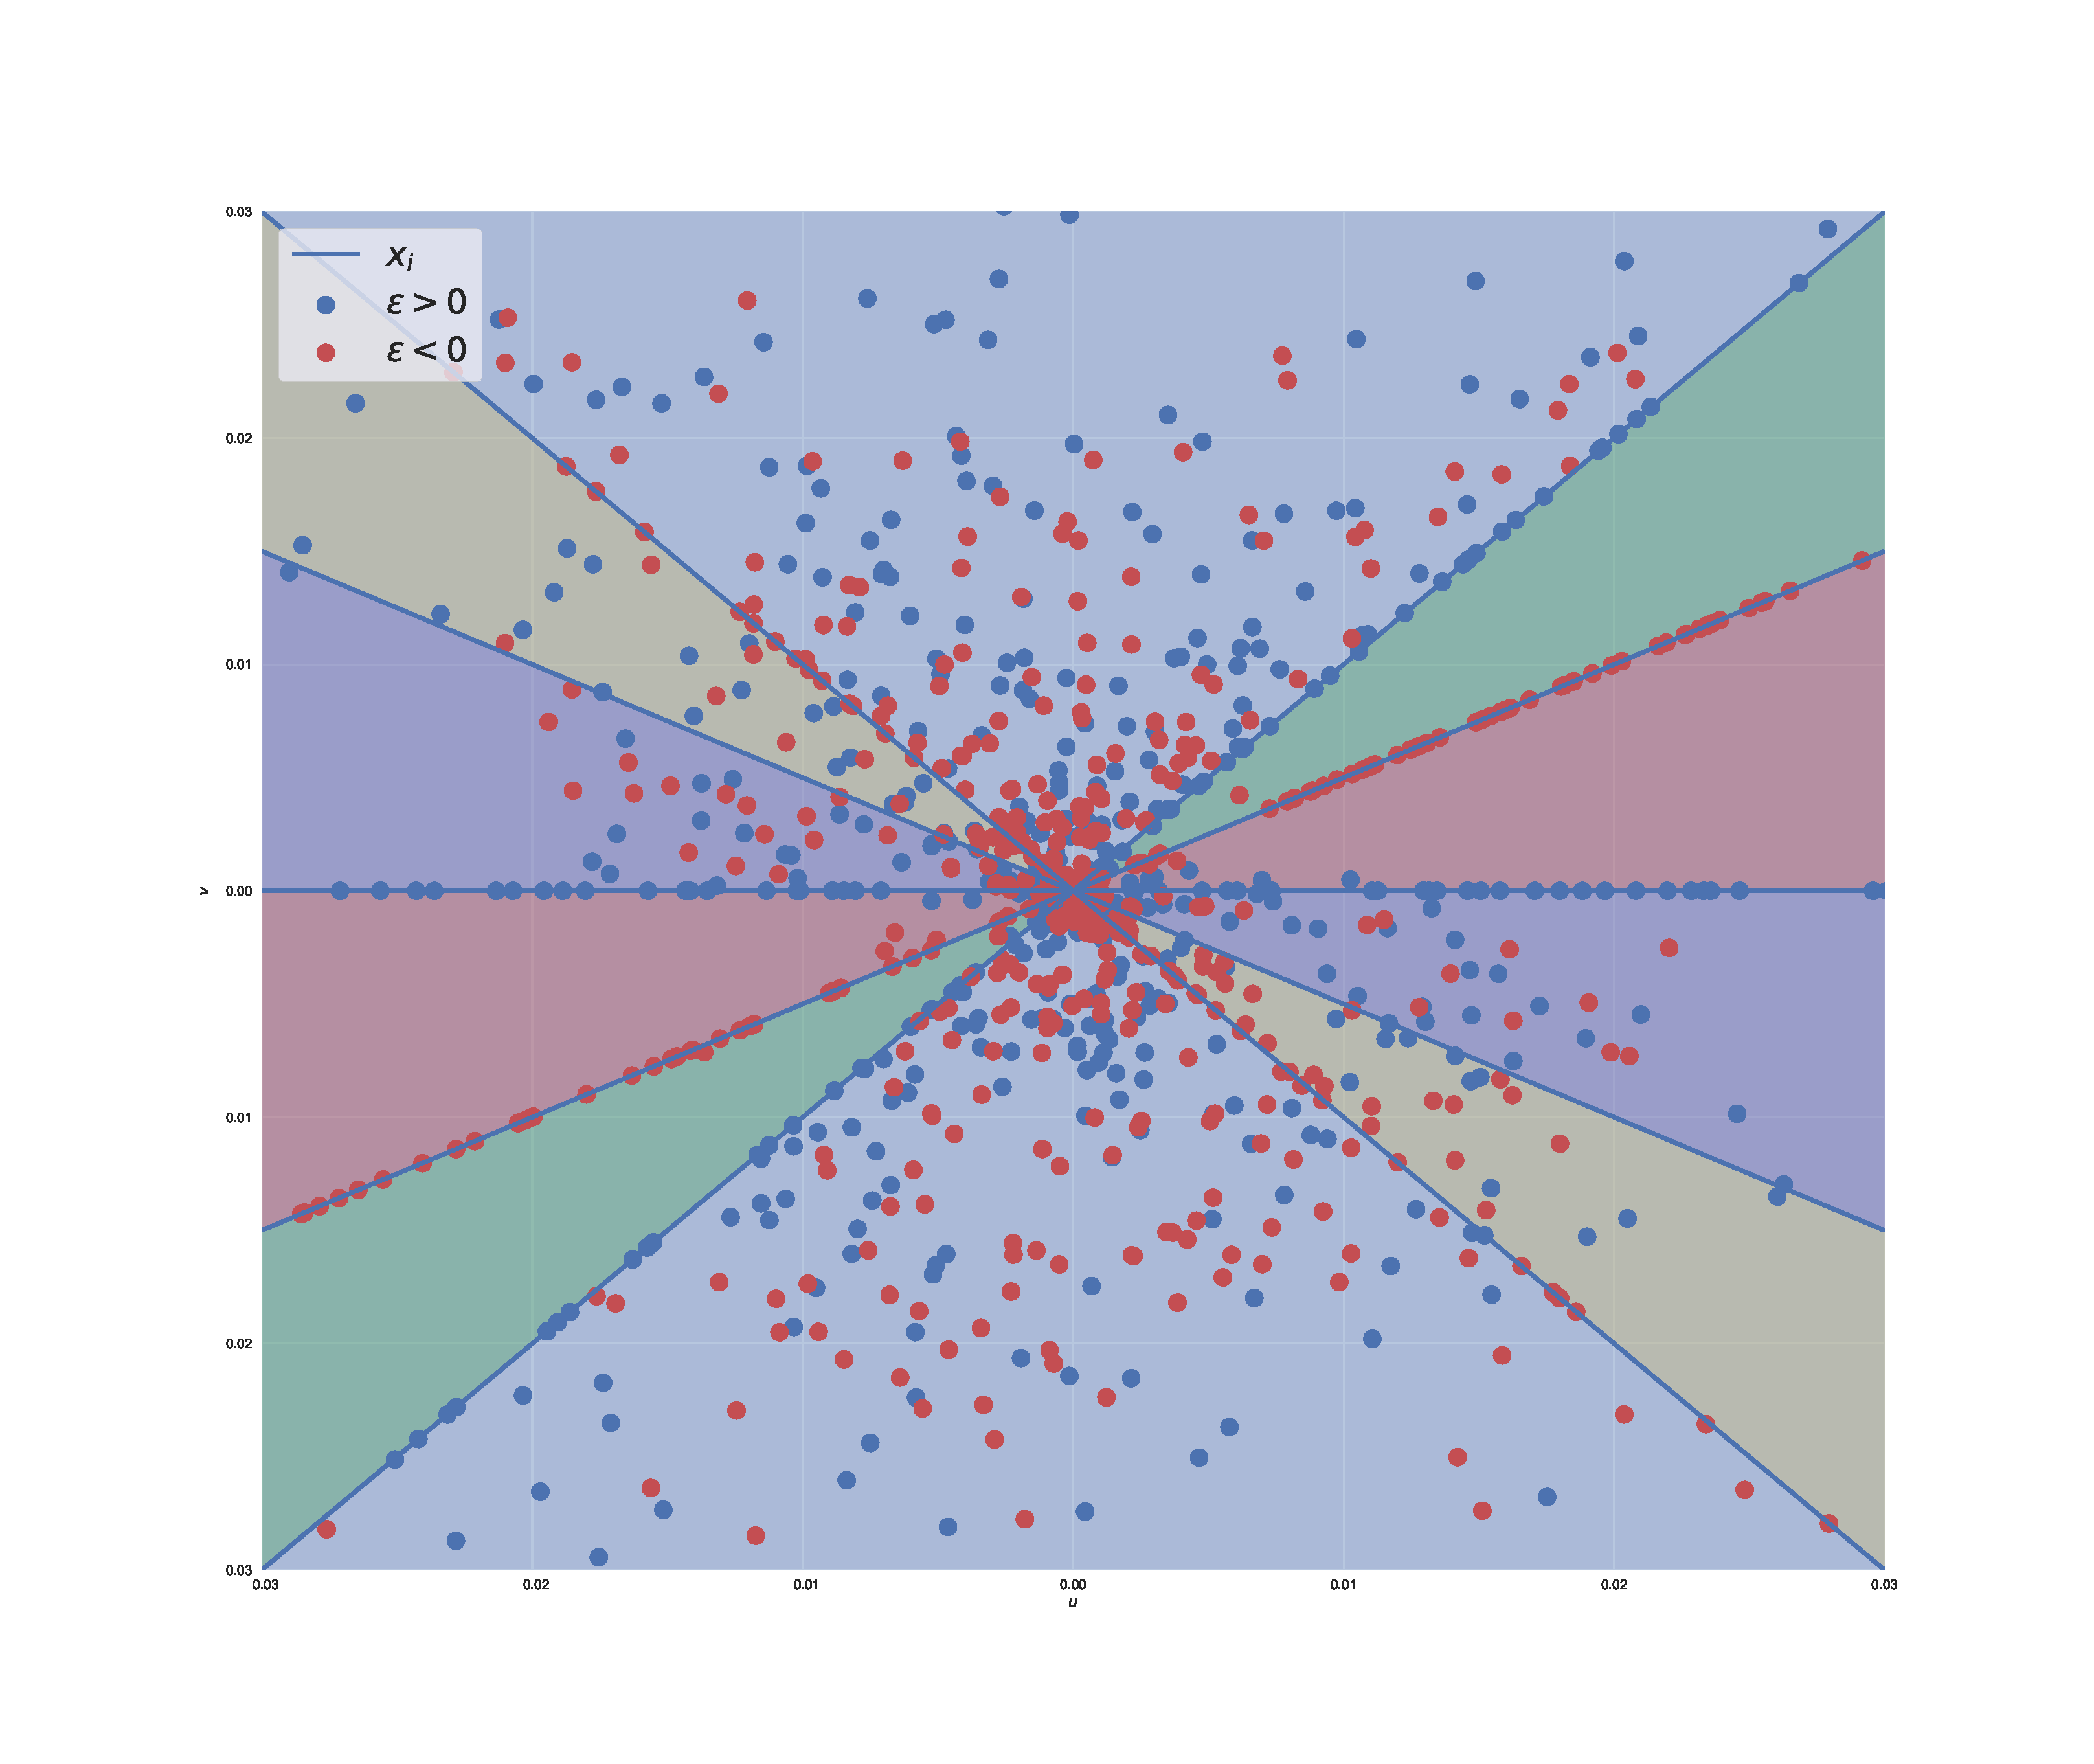
\includegraphics[width=\linewidth]{figures/reduced_gradient_phase.pdf}
    \endminipage
    \minipage{0.33\textwidth}
        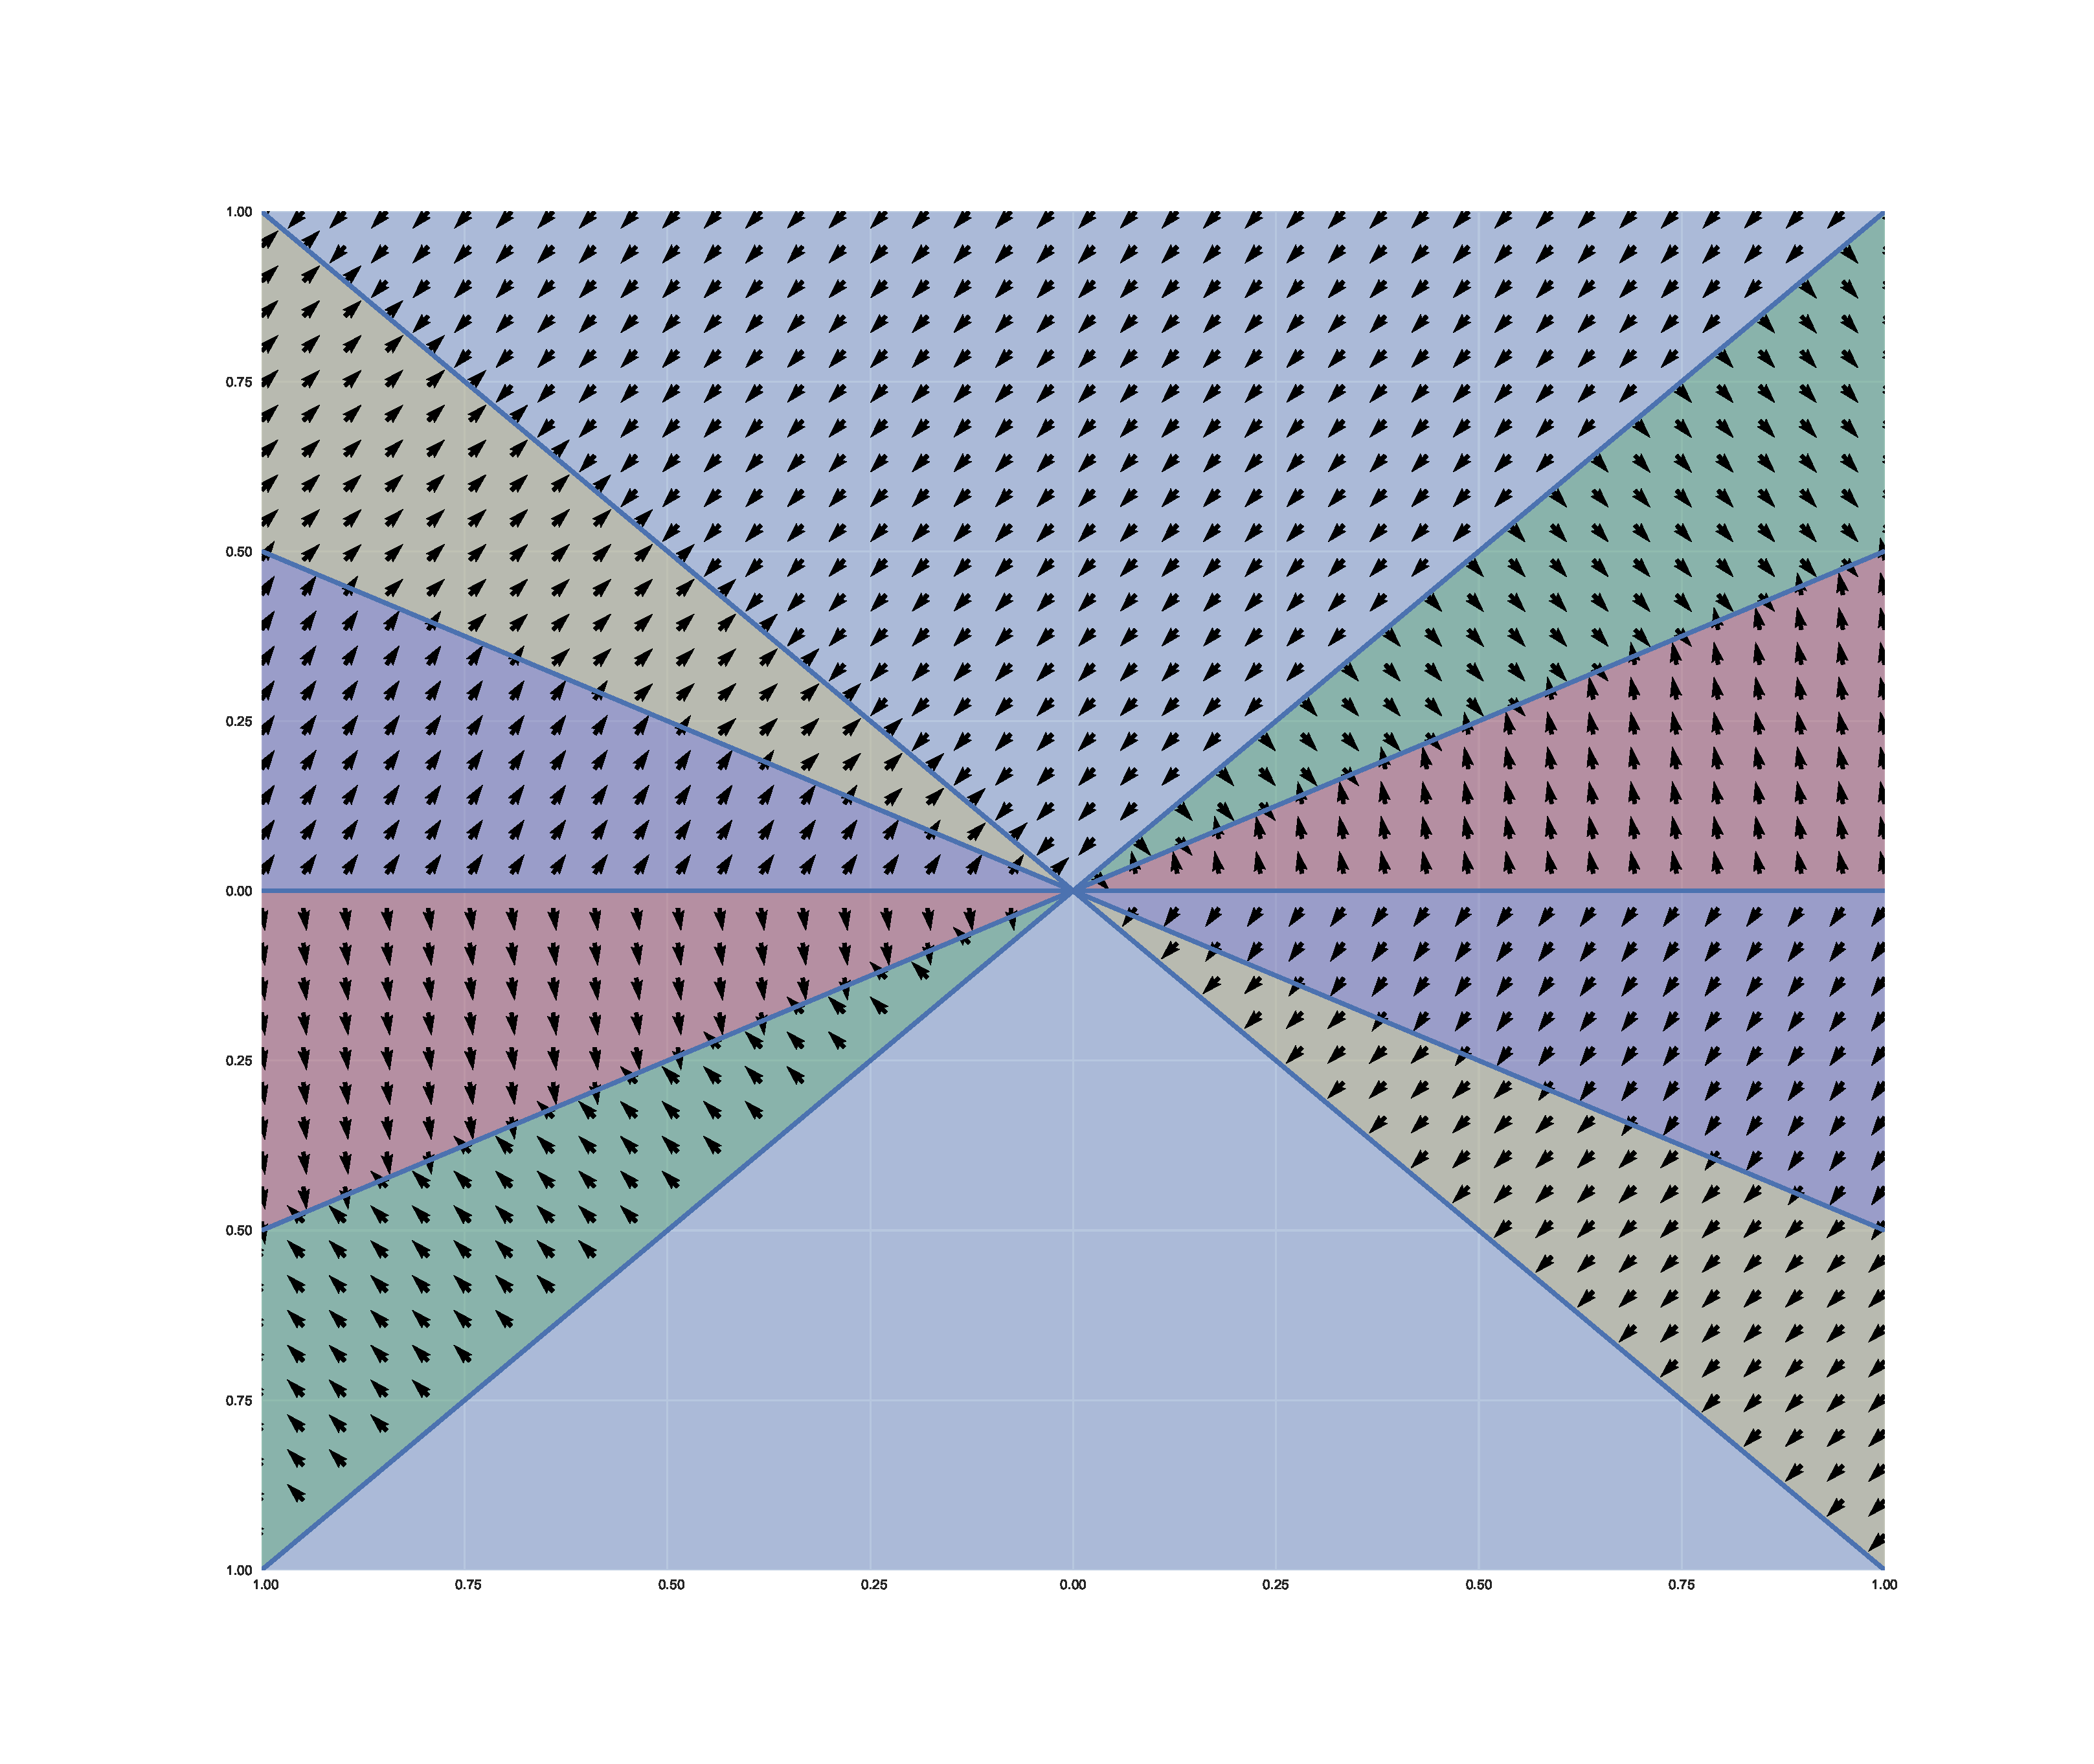
\includegraphics[width=\linewidth]{figures/reduced_gradient_vector_field.pdf}
    \endminipage\hfill
    \caption{The vector field of the gradient of the loss in reduced parameter space $\nabla \tilde{L}(\bm \xi)$. Note that the orientation of the arrow depends on the sign $\epsilon_i$ of a neuron. Thus, the gradient of the blue neurons are the arrows in the picture while the gradient of the red neurons point point in the opposite direction. We see in the middle image, that the neurons cluster on different samples depending on their sign.}
    \label{fig:reduced_grad}
\end{figure}

which is a piecewise constant function with the boundary between pieces occuring along the sample lines $u x_j + v = 0, j = 1 \ldots s$ (see Figure~\ref{fig:reduced_grad}). While the gradient field is in general discontinuous on the boundary of a sample, the component along a sample line is continuous

\begin{lemma}
The component of the gradient field $\nabla \tilde{L}(\xi)$ along a line $l : u x_j + v = 0$ is continuous in any open neighborhood centered on $l$.
\end{lemma}

We see from \eqref{eq:grad_reduced} that $\nabla \tilde{L}$ at a point $(u_i, v_i, \epsilon_i)$ is a linear combination of the sample vectors $(x_j, 1)^T$  weighted by the residual $f_{\bm \xi}(x_j) - y_j$ with a possible sign flip depending on $\epsilon_i$. Thus depending on $\epsilon_i$ and the signs of the residuals at the samples, $\nabla \tilde{L}$ for a specific neuron could point in opposing directions along a sample boundary. In the cases, where the vector field points towards the sample line on either side, neurons will ``stick'' to the sample boundary. In fact, we show that for every possible neuron, there is at least one ``sticky'' sample to which it is attracted. Note that these ''sticky`` samples may change over time as the residual evolves and as the signs of neurons change. Below we give a condition for a sample to be attract a neuron. 

\begin{lemma}
Given a set of samples $\bm x = (x_j)_{j=1}^s$ and labels $\bm y = (y_j)_{j=1}^s$, then for any given residual and sign $\epsilon$, there is a nonempty set $S$ of samples $x_j$ which are sticky. \note{(this is super informal but I want to get a quick draft of the section, we should write out explicitly that the gradient field along the sample boundary is pointing in opposite directions )}
\end{lemma}

\todo{The attractiveness of samples only depends on the number of samples, neurons concentrate along sample lines , condition for attractiveness, clustering acts as a regularizer favoring piecewise linear functions.}
\begin{figure}
    \centering
    \minipage{0.33\textwidth}
    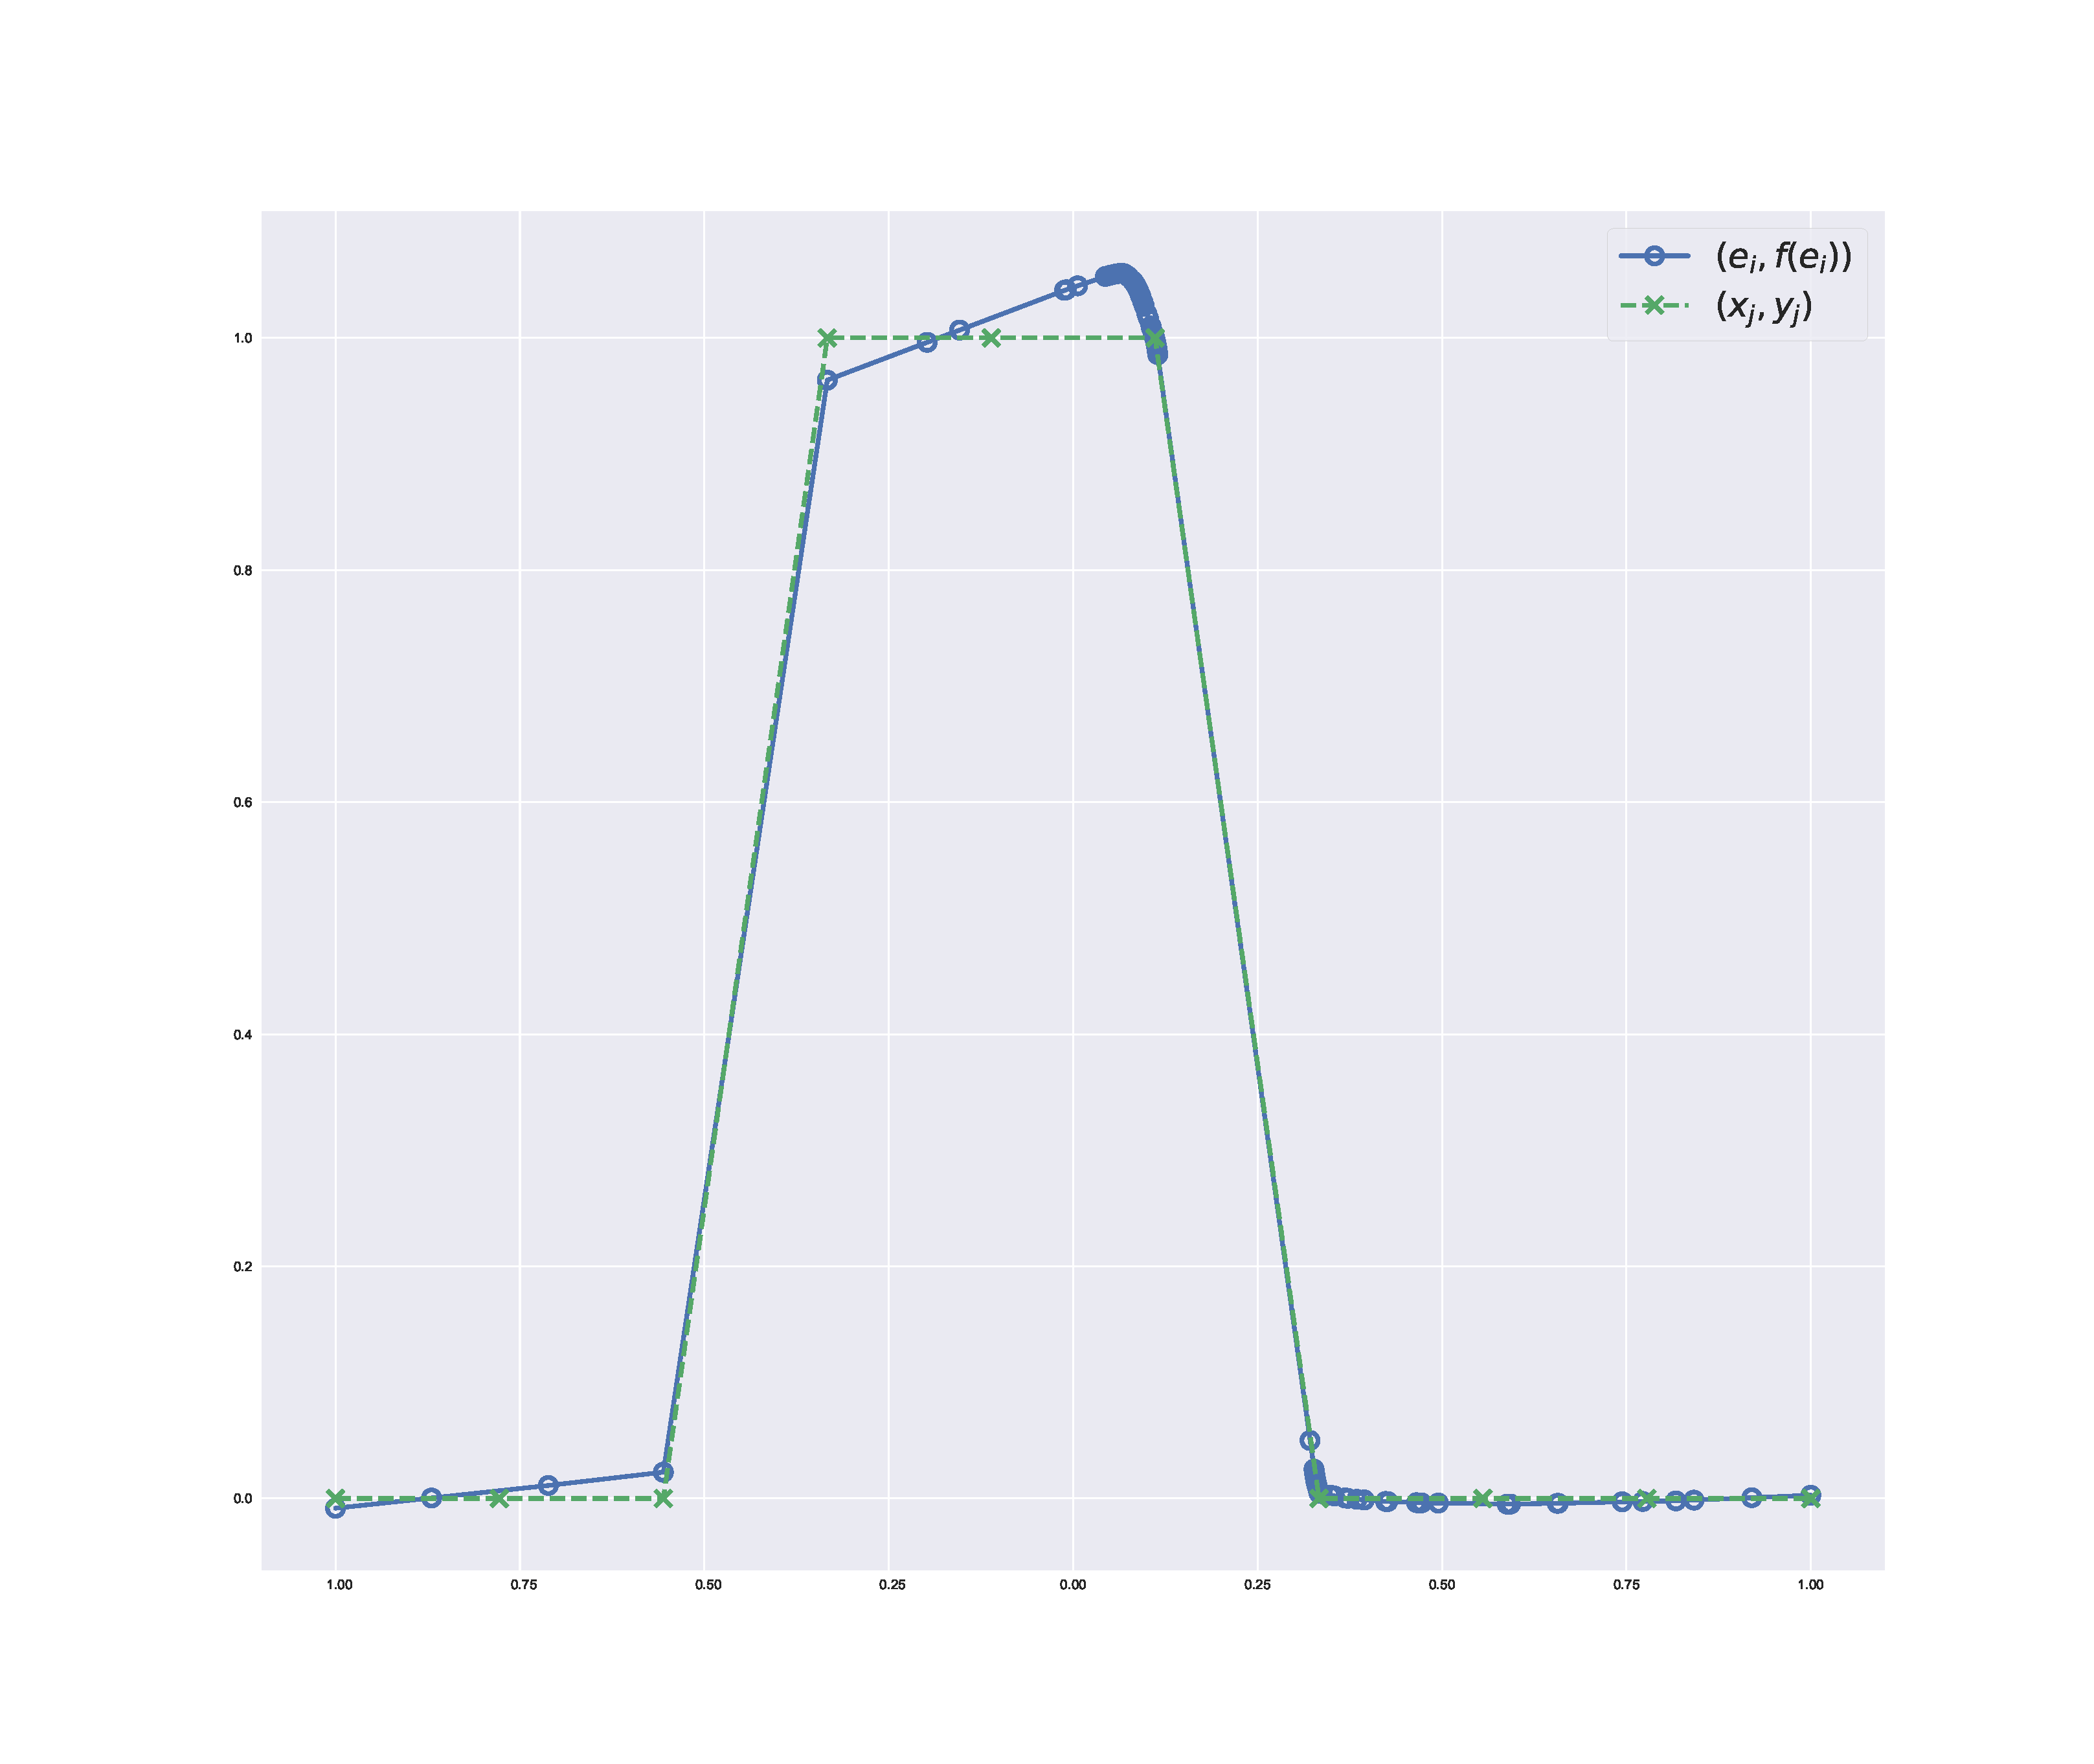
\includegraphics[width=\linewidth]{figures/neuron_trajectories_recon.pdf}
    \endminipage\hfill
    \minipage{0.33\textwidth}
    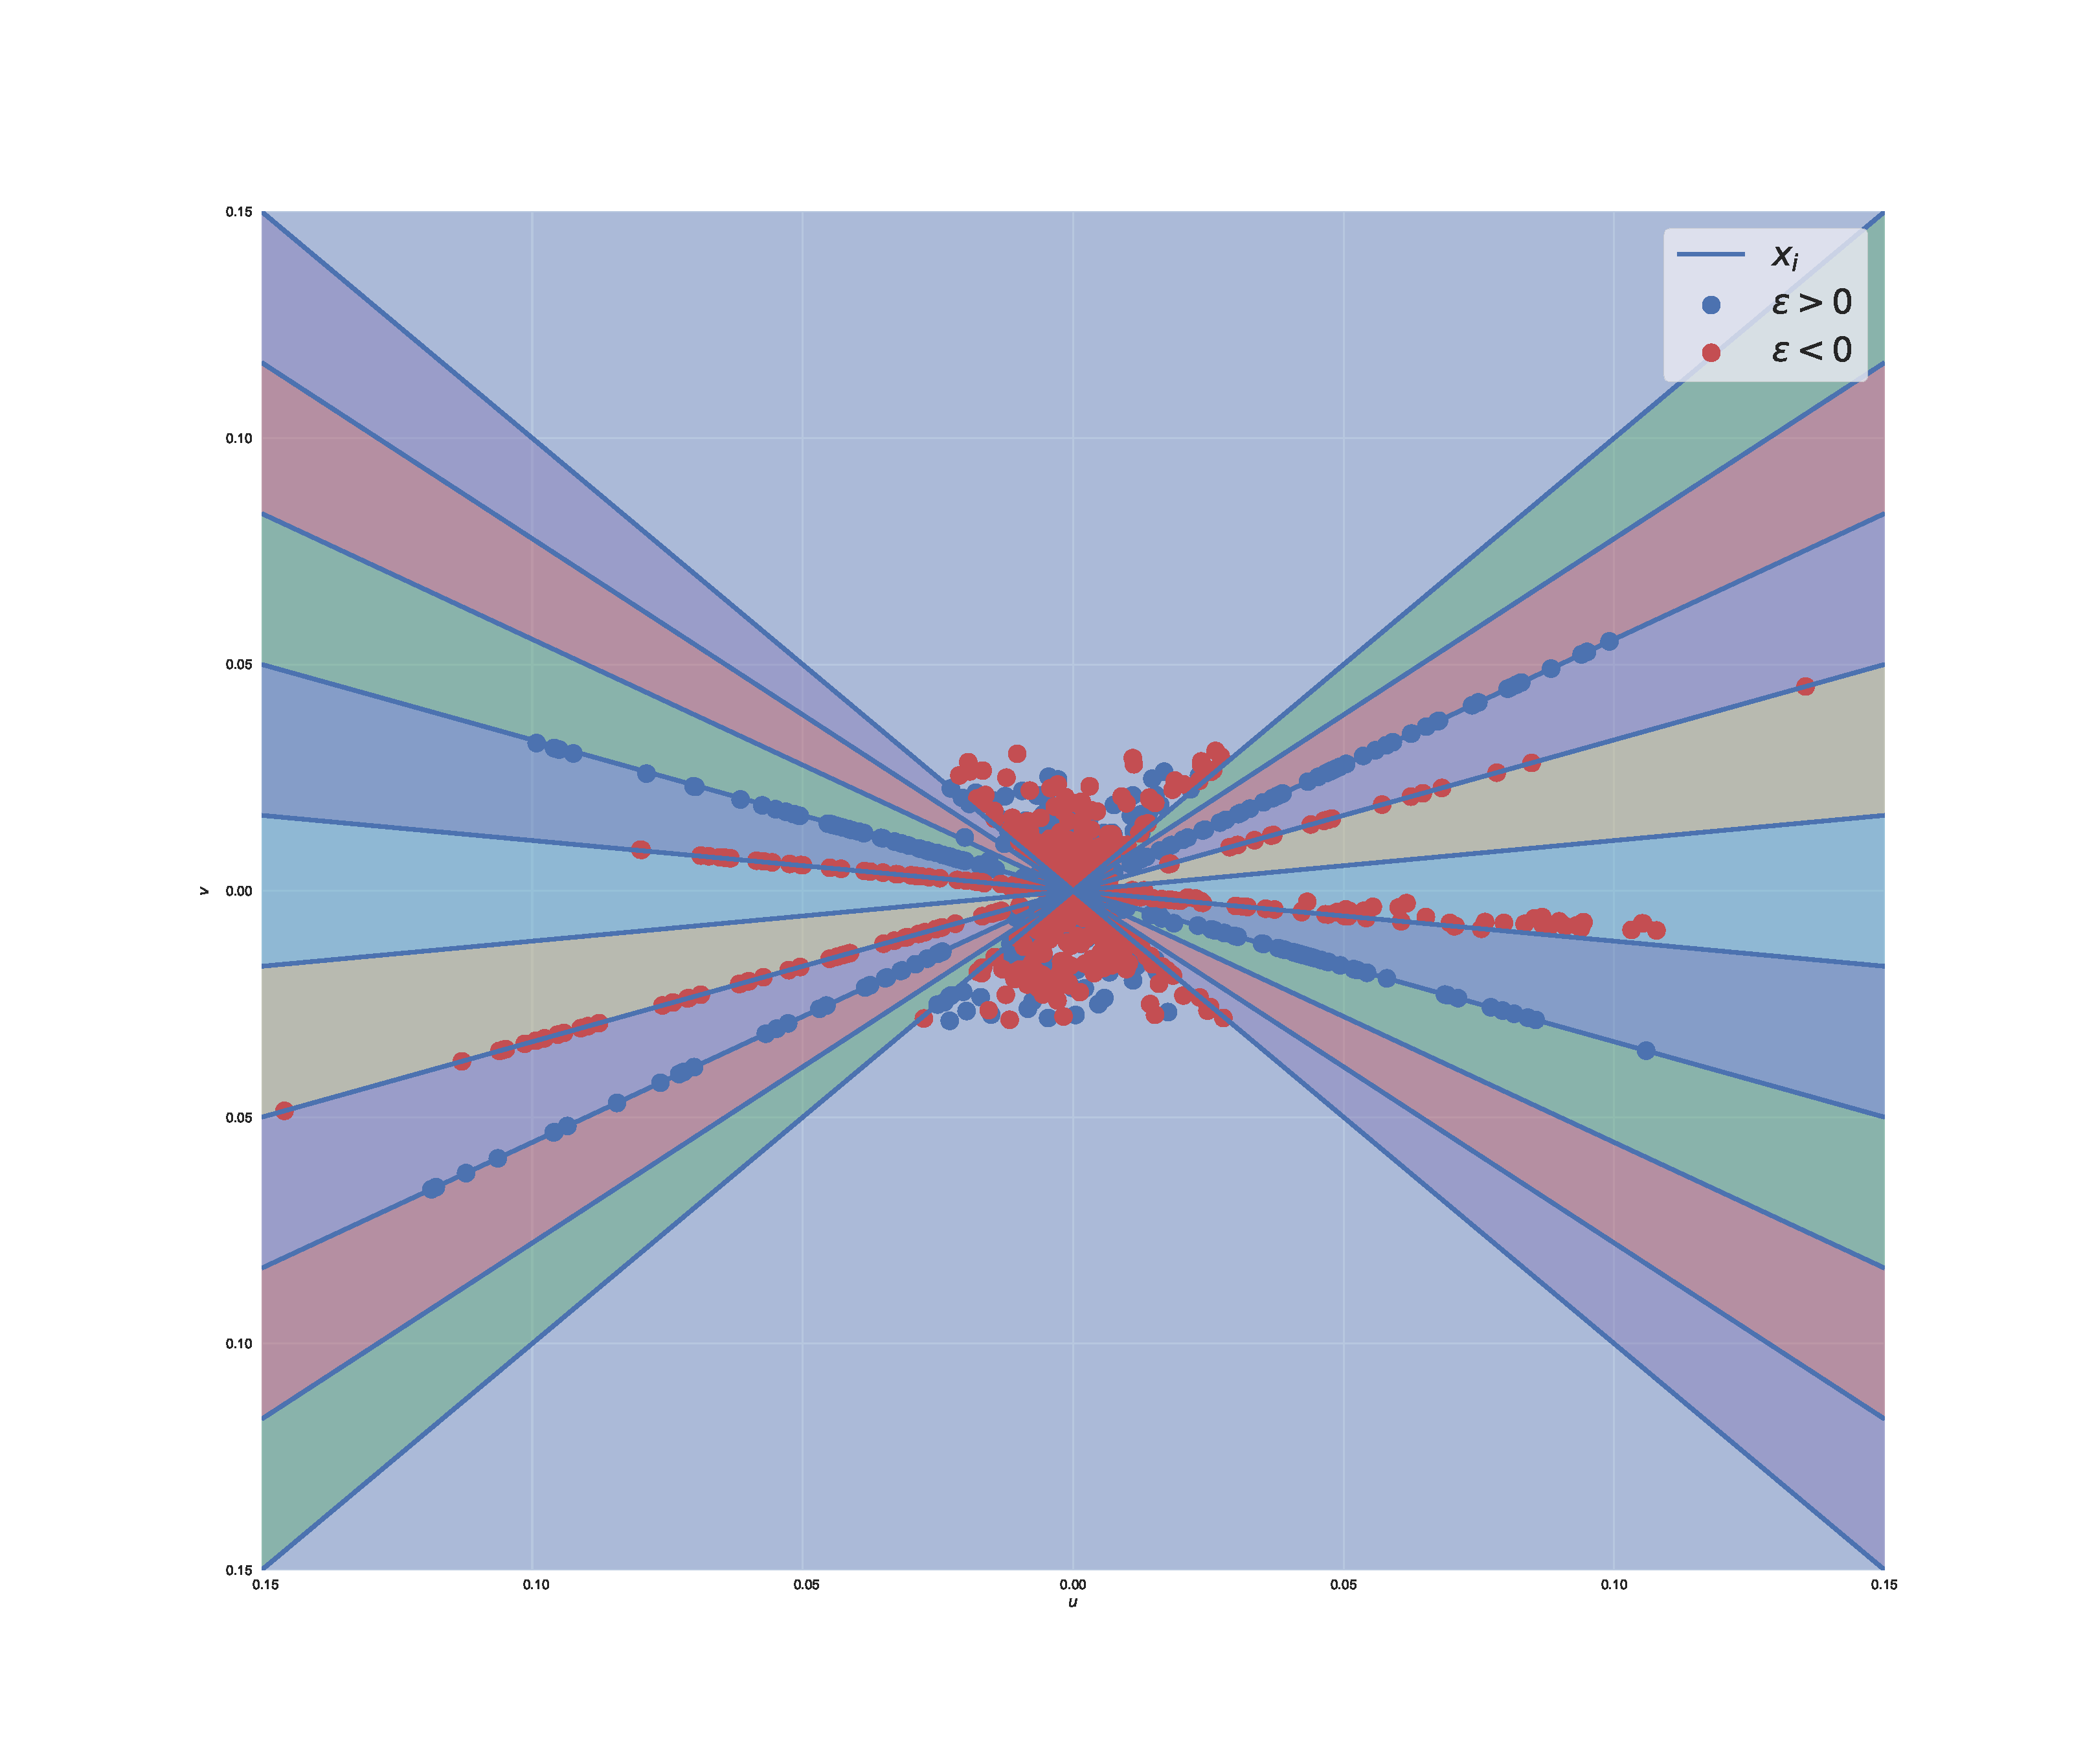
\includegraphics[width=\linewidth]{figures/neuron_trajectories_phase.pdf}
    \endminipage\hfill
    \minipage{0.33\textwidth}
    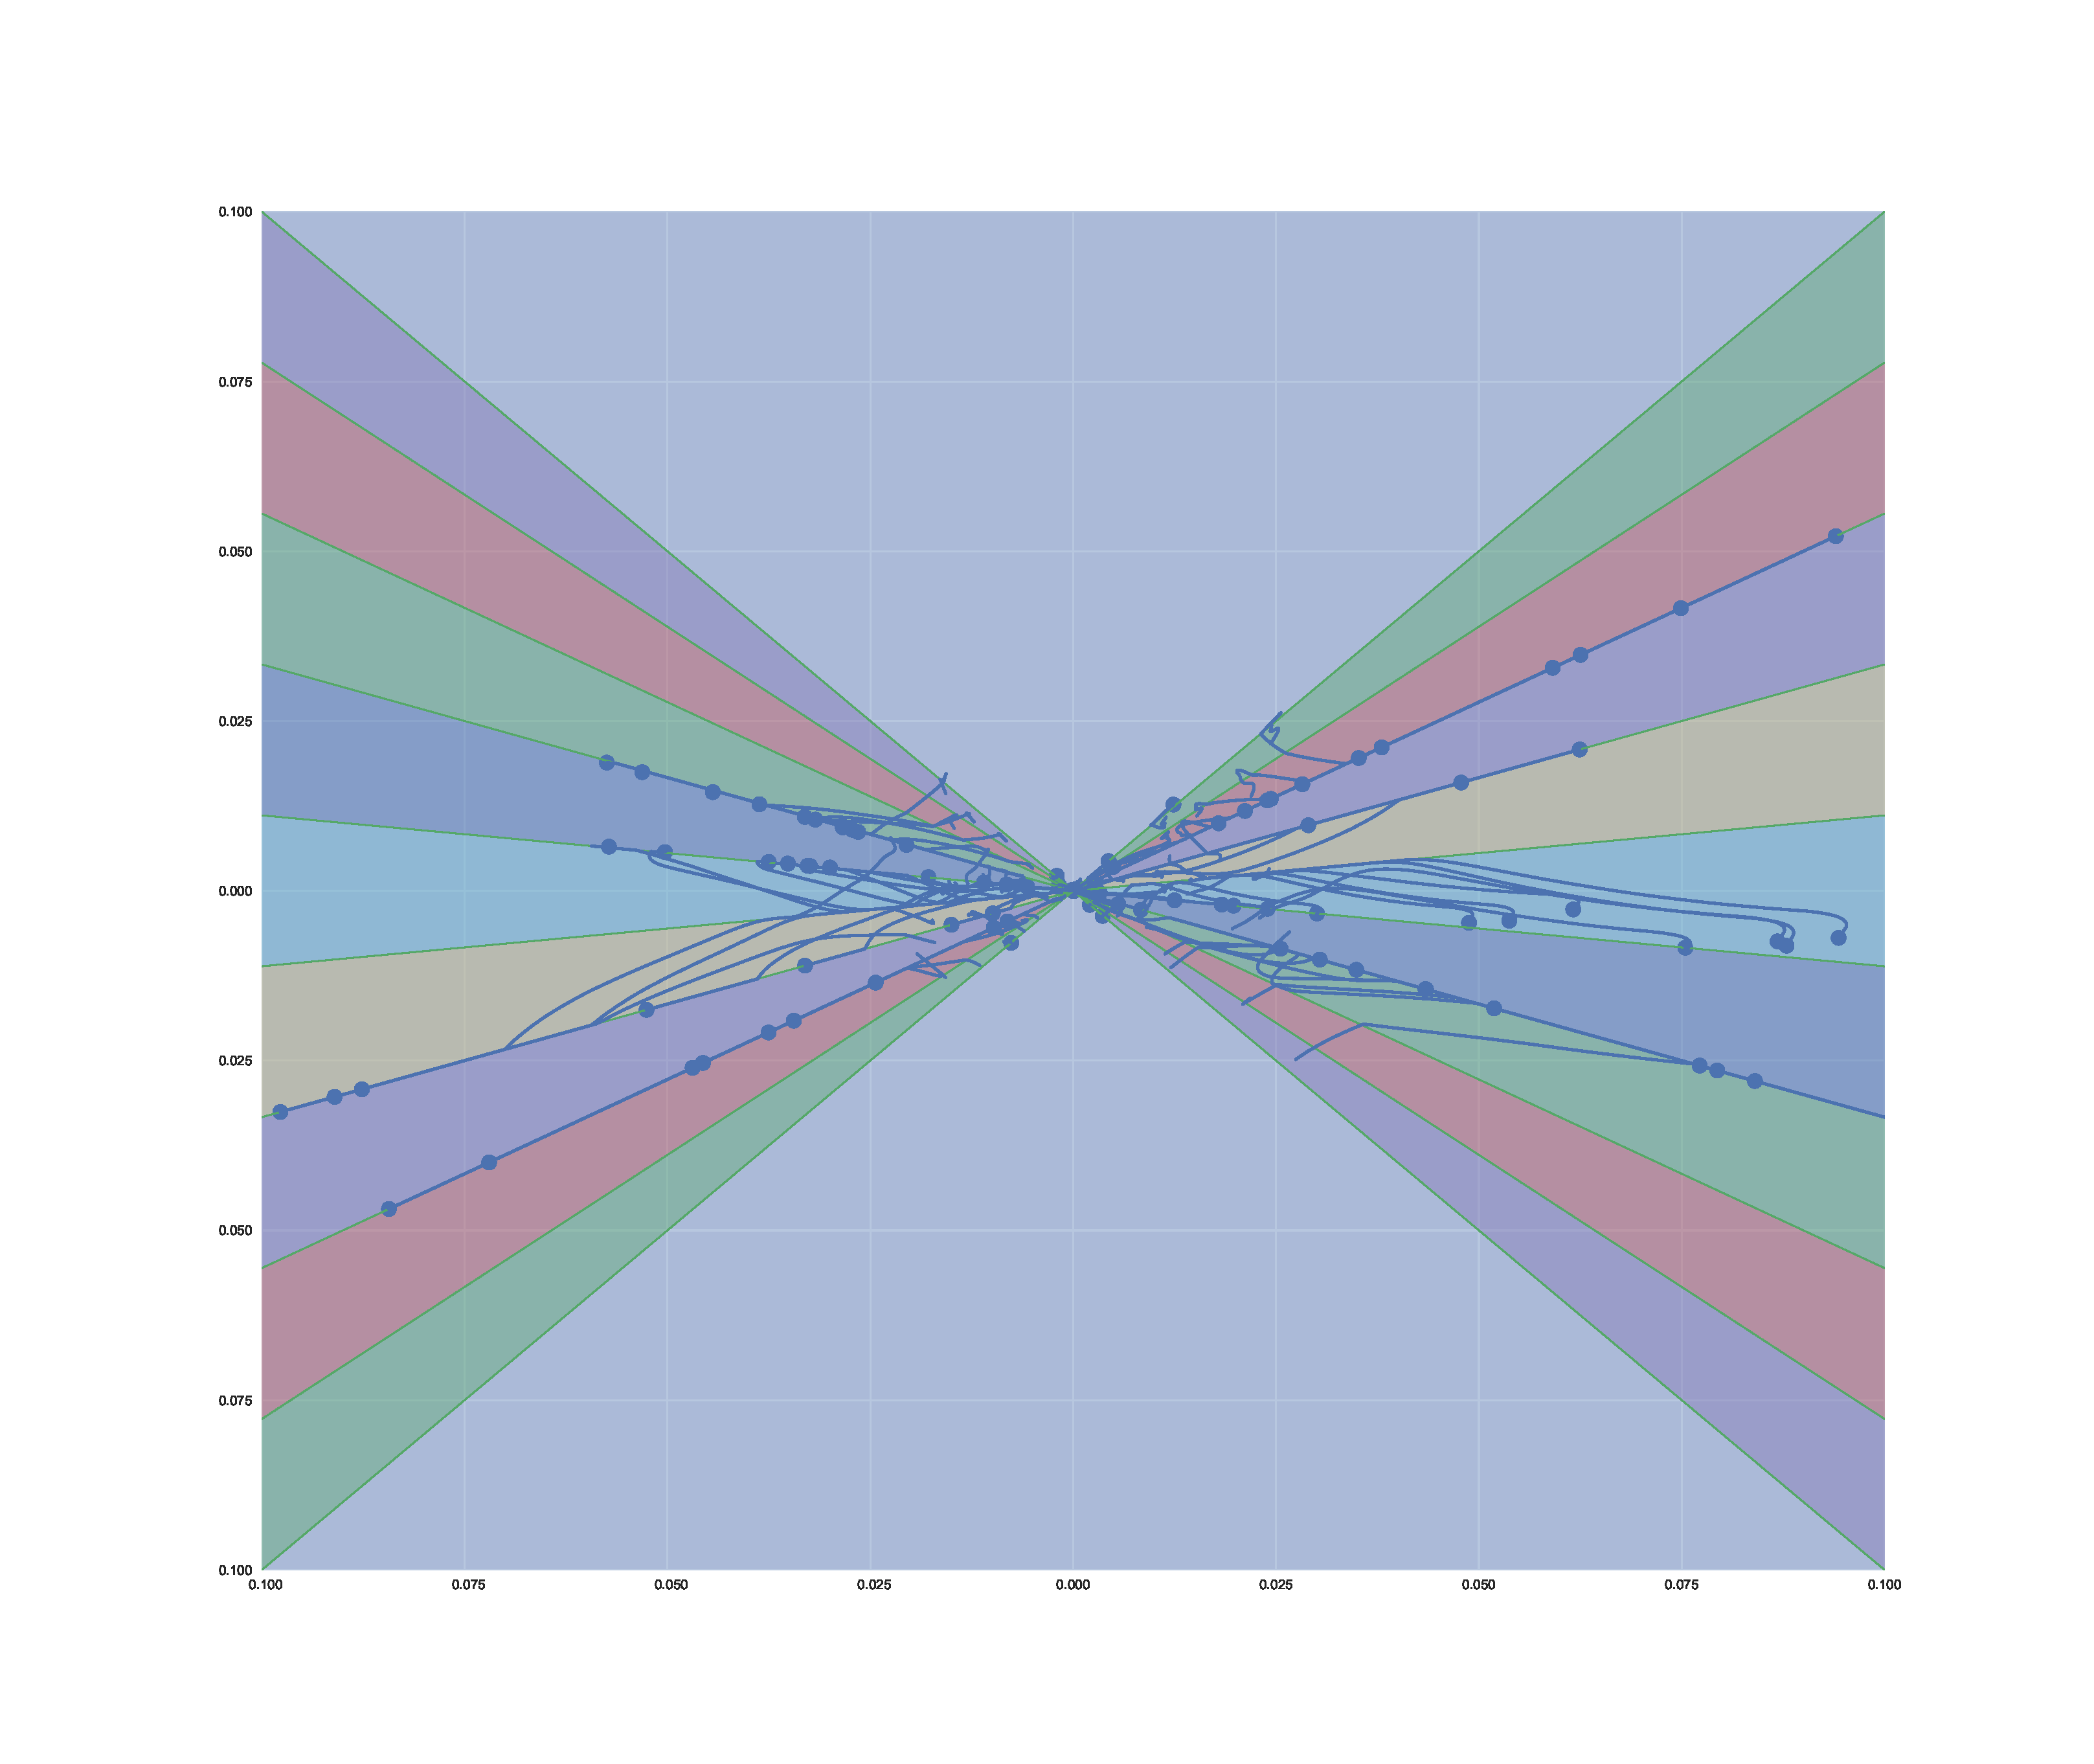
\includegraphics[width=\linewidth]{figures/neuron_trajectories.pdf}
    \endminipage
    \caption{Evolution of neurons in the tangential regime while fitting a square wave with 1000 neurons. The left image shows the trained network on and sample points. The middle image shows the distribution of all neurons at the end of training. The right image shows trajectories for a random sample of 100 neurons. Observe how in this regime, neurons concentrate on certain samples. The trajectories in this case get stuck at the sample boundary.}
    \label{fig:tangential_trajectories}
\end{figure}


\begin{figure}
    \centering
    \minipage{0.33\textwidth}
    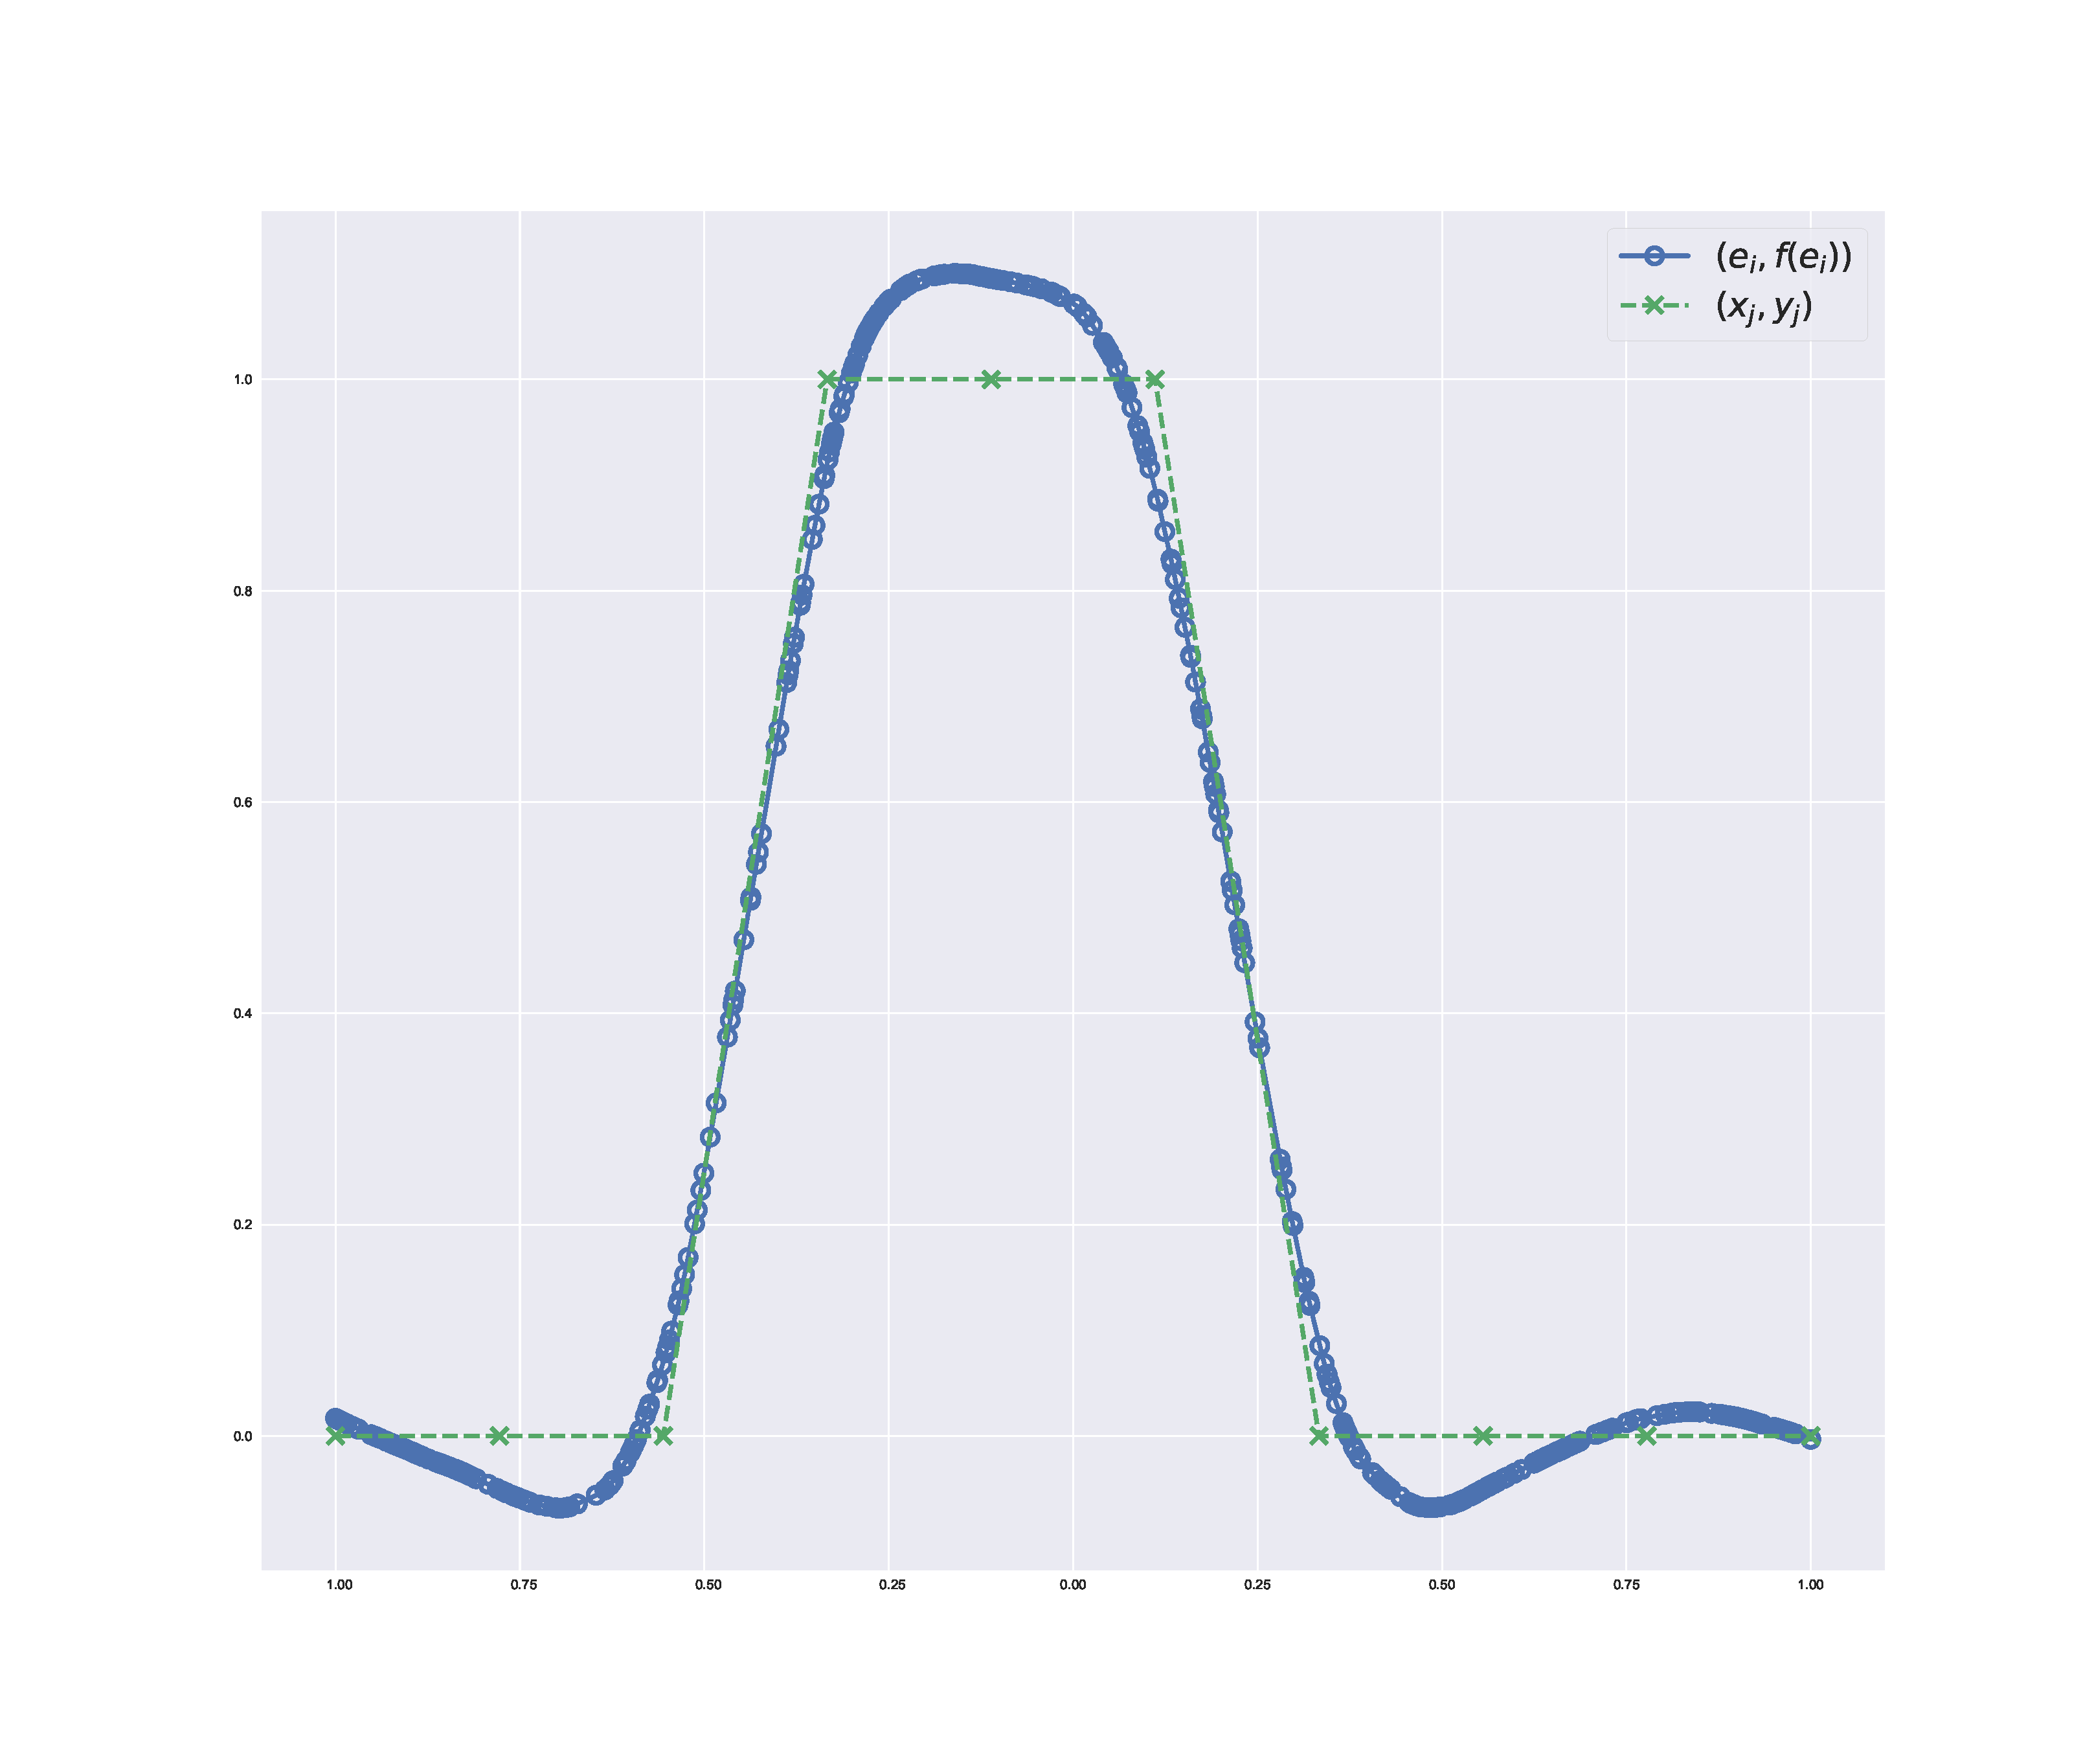
\includegraphics[width=\linewidth]{figures/radial_trajectories_recon.pdf}
    \endminipage\hfill
    \minipage{0.33\textwidth}
    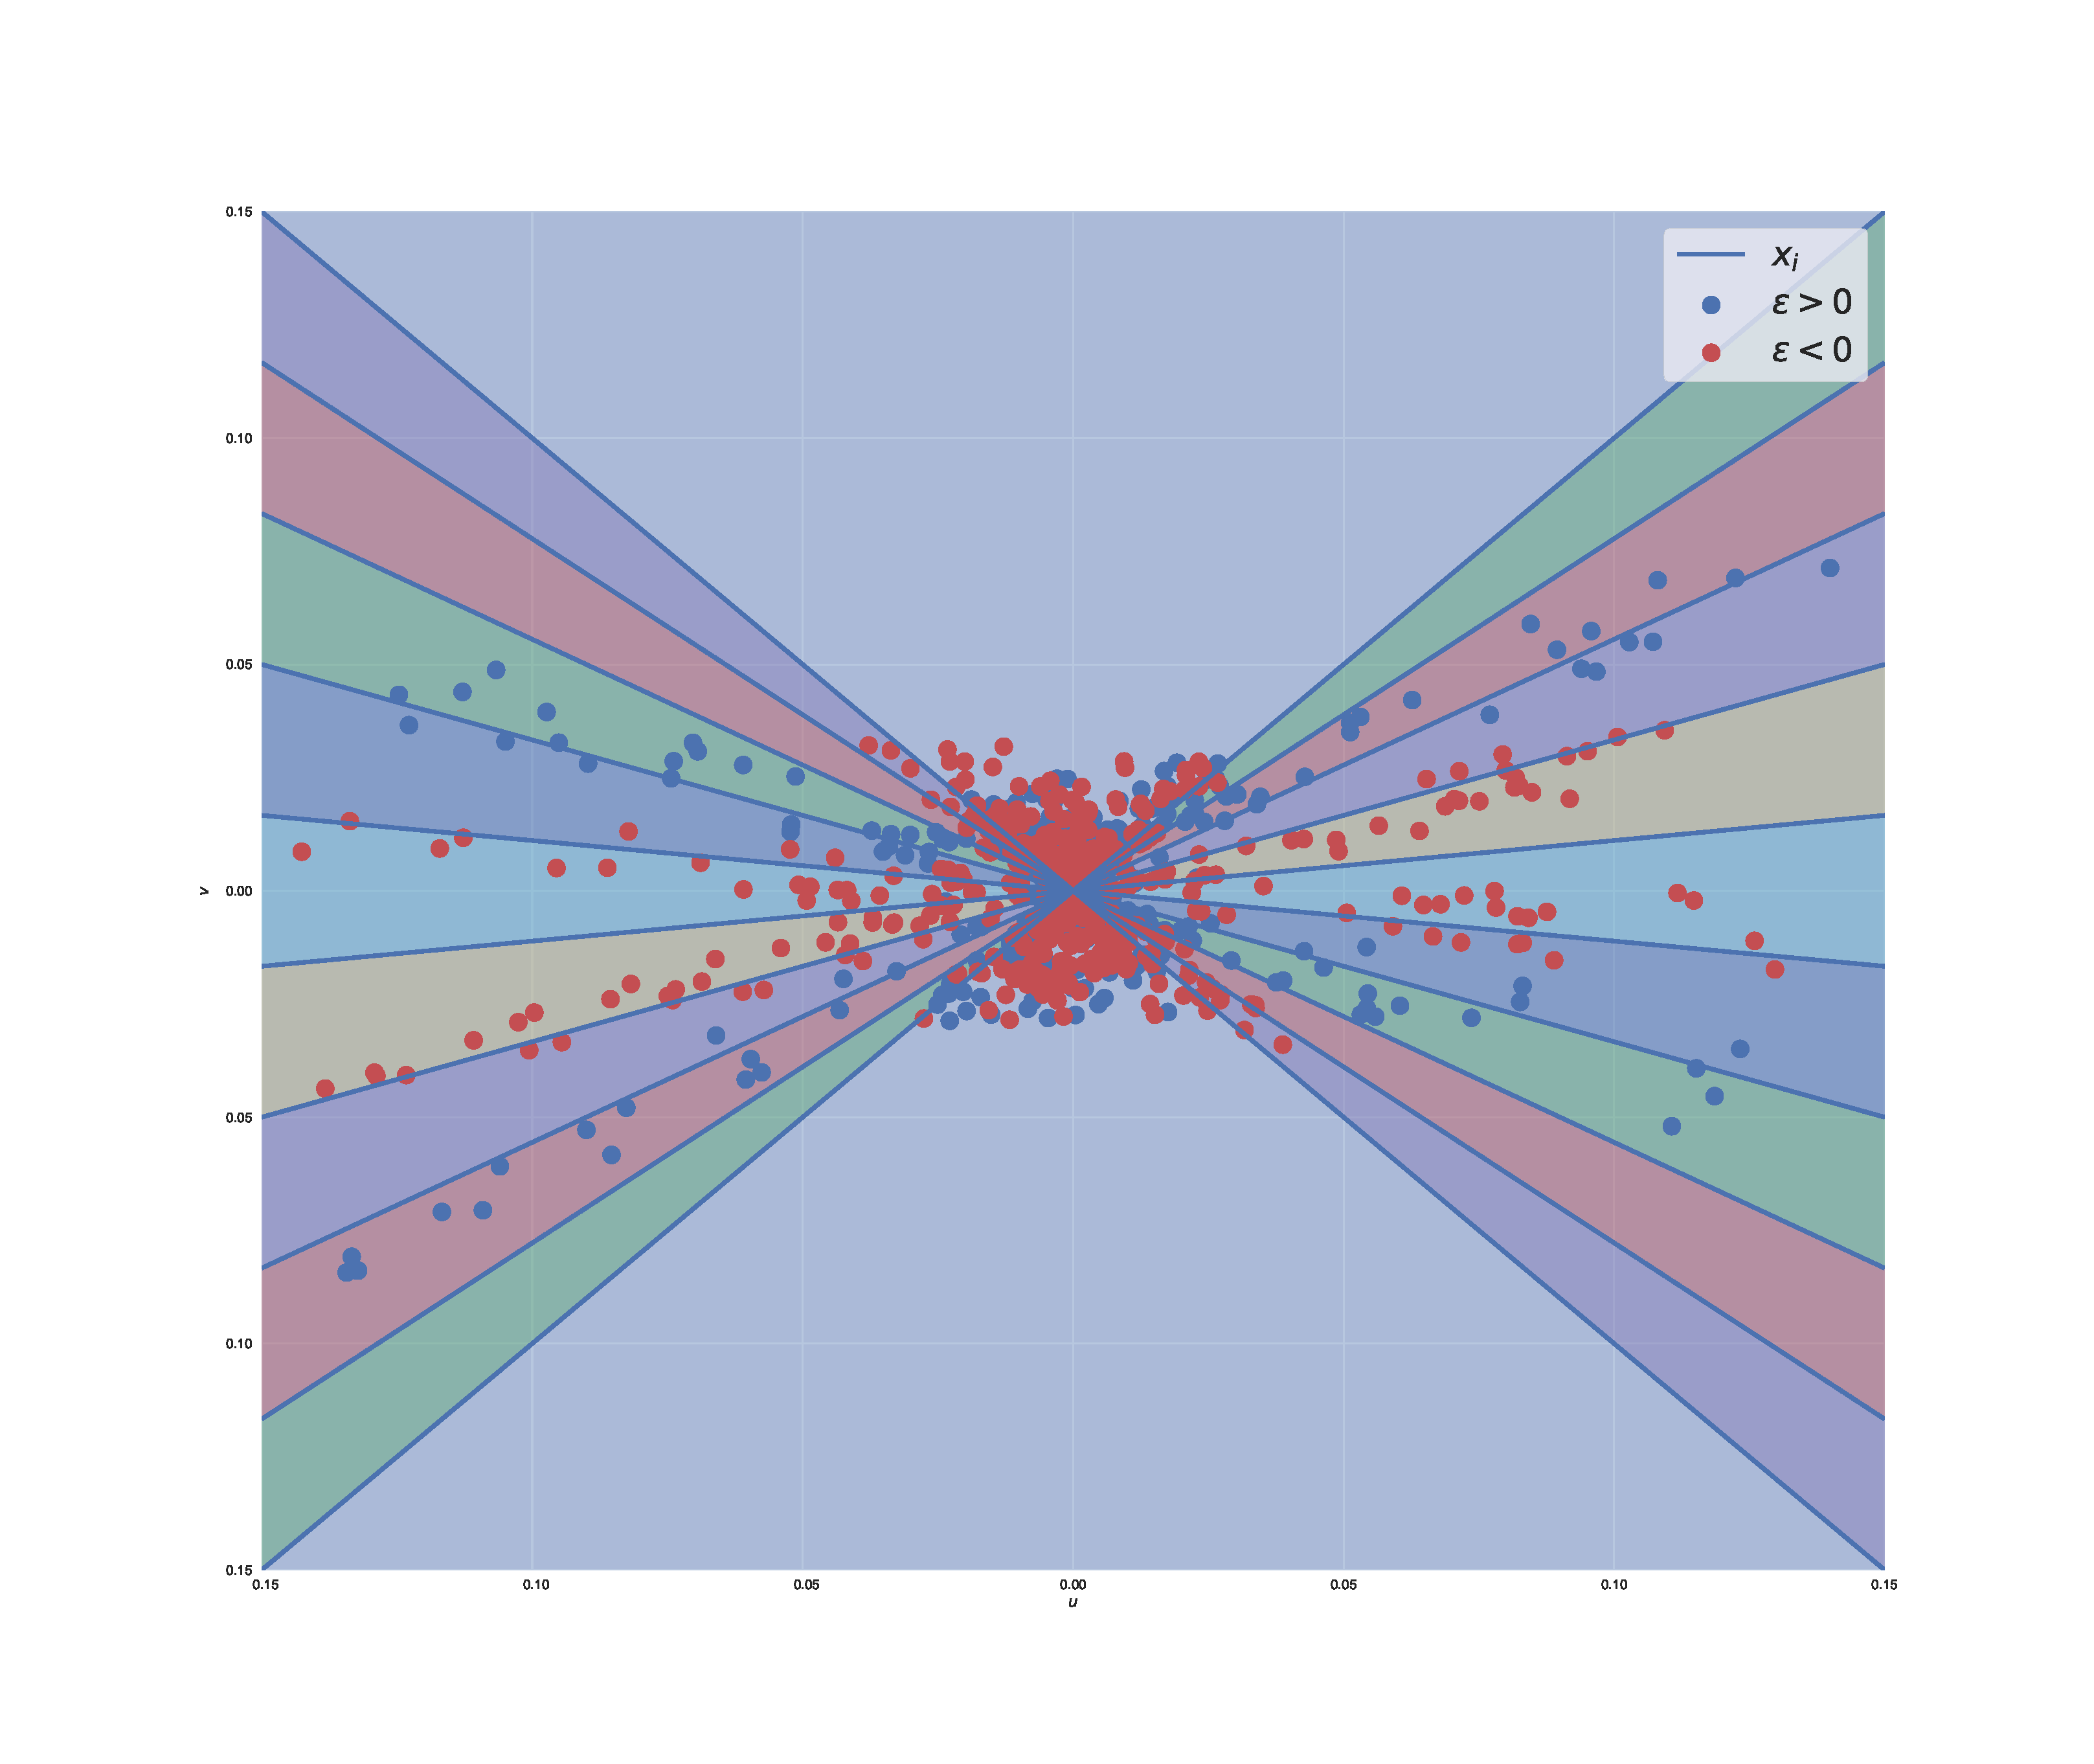
\includegraphics[width=\linewidth]{figures/radial_trajectories_phase.pdf}
    \endminipage\hfill
    \minipage{0.33\textwidth}
    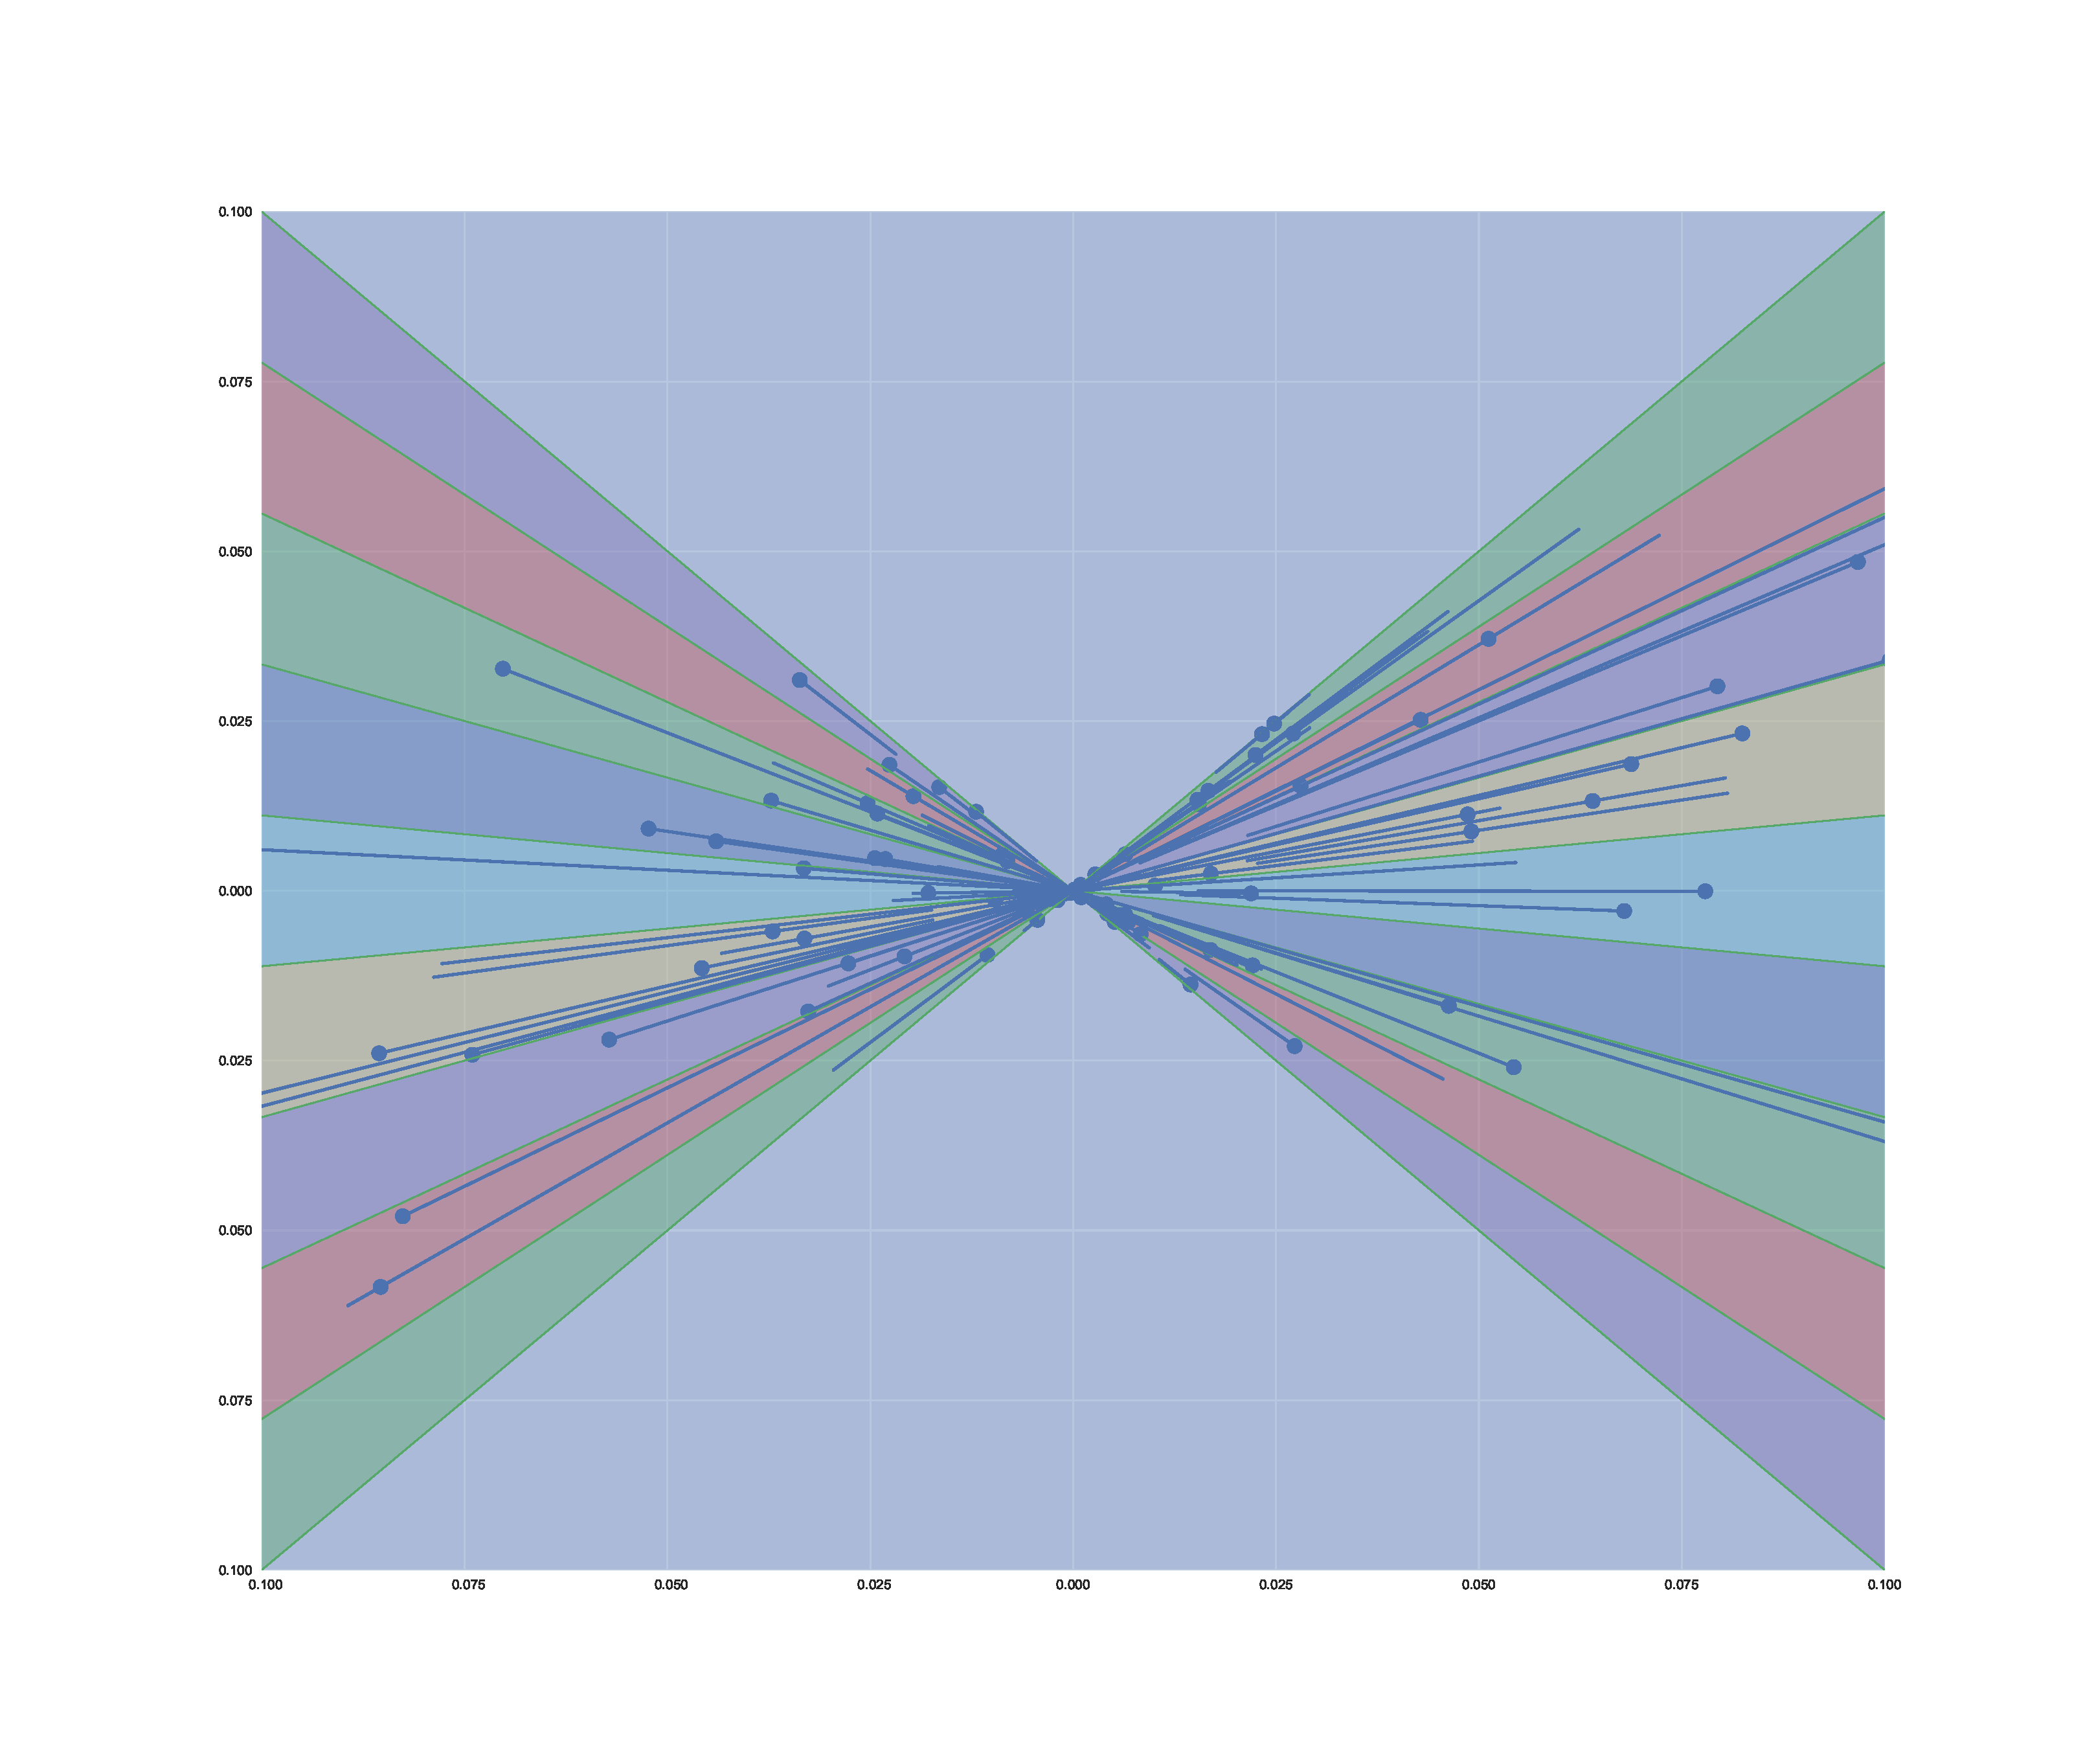
\includegraphics[width=\linewidth]{figures/radial_trajectories.pdf}
    \endminipage
    \caption{Evolution of neurons in the radial regime while fitting a square wave with 1000 neurons. The left image shows the trained network on and sample points. The middle image shows the distribution of all neurons at the end of training. The right image shows trajectories for a random sample of 100 neurons.}
    \label{fig:radial_trajectores}
\end{figure}


